A common, baseline selection is applied for the resonant  analyses of the 2015 and 2016 data that is taken directly from ~\cite{Bauce:2226443}, as described in Section~\ref{sec:base_selection}. Then, specific cuts applied
for the resonant analysis, tailored to improve the sensitivity, are described in Sections~\ref{sec:res_selection}. 

\subsection{Baseline selection}
\label{sec:base_selection}
The baseline event selection is applied for both analyses and
the cuts applied are:
\begin{itemize}
\label{item:basicSelection}
\item Good Run List (GRL): Requirement that all relevant detectors were in a good state ready for physics
\item LAr: Liquid Argon Calorimeter error rejected ( errorState(xAOD::EventInfo::LAr) )
\item Tile: Tile Calorimeter error rejected ( errorState(xAOD::EventInfo::Tile) )
\item SCT: SCT single event upsets rejected ( errorState(xAOD::EventInfo::SCT) )
\item Core: Incomplete event build rejected ( isEventFlagBitSet(xAOD::EventInfo::Core, 18) )
\item Primary Vertex: the highest $\sum\pt^{2}(trk)$ (xAOD::VxType::VertexType::PriVtx) vertex has at least two tracks associated with it
\item Trigger: passes HLT\_j380 (Section~\ref{sec:trigger})
\item All jets with $\pt>60~\GeV$ pass cleaning cuts
\item Leading jet $\pt>440~\GeV$
\item Subleading jet $\pt>60~\GeV$
\end{itemize}

Additional kinematic selection criteria are used for the resonance and angular search distributions separately to optimise the search potential.


\subsection{Resonance Analysis Specific Cuts}
\label{sec:res_selection}
On top of the cuts listed in~\ref{sec:base_selection}
the following cuts are applied to the resonance search:
\begin{itemize}
\item $|y^*| < 0.6$
\item $\mjj > 1100~\GeV$ %(Table~\ref{tab:trigCuts})
\end{itemize}
for all the benchmark signals except for W*.

%Give its different decay topology, for the search of W* signal slightly different cuts are applied, 
%motivated in ~\ref{sec:Wstar_CutOptimisation}:
%\begin{itemize}
%\item $|y^*| < 1.2$
%\item $\mjj > 1717~\GeV$
%\end{itemize}

%The optimisation of these cuts is described in Section~\ref{sub:phaseSpace}. 

\subsection{Basic kinematic plots}
\label{sec:kinematic_distributions}

%In this section a selection of kinematic and monitoring plots produced with the resonant selection on the full dataset is shown 
%(Figures~\ref{fig:monitoring1}, %\ref{fig:monitoring2}, \ref{fig:monitoring3}, 
%\ref{fig:monitoring5}, \ref{fig:monitoring6}). These plots are relative to \integLumi of data collected in 2015 and 2016.
% GRL has been applied here.
%
%\begin{figure}[htb]
% \centering
% \subfigure[] {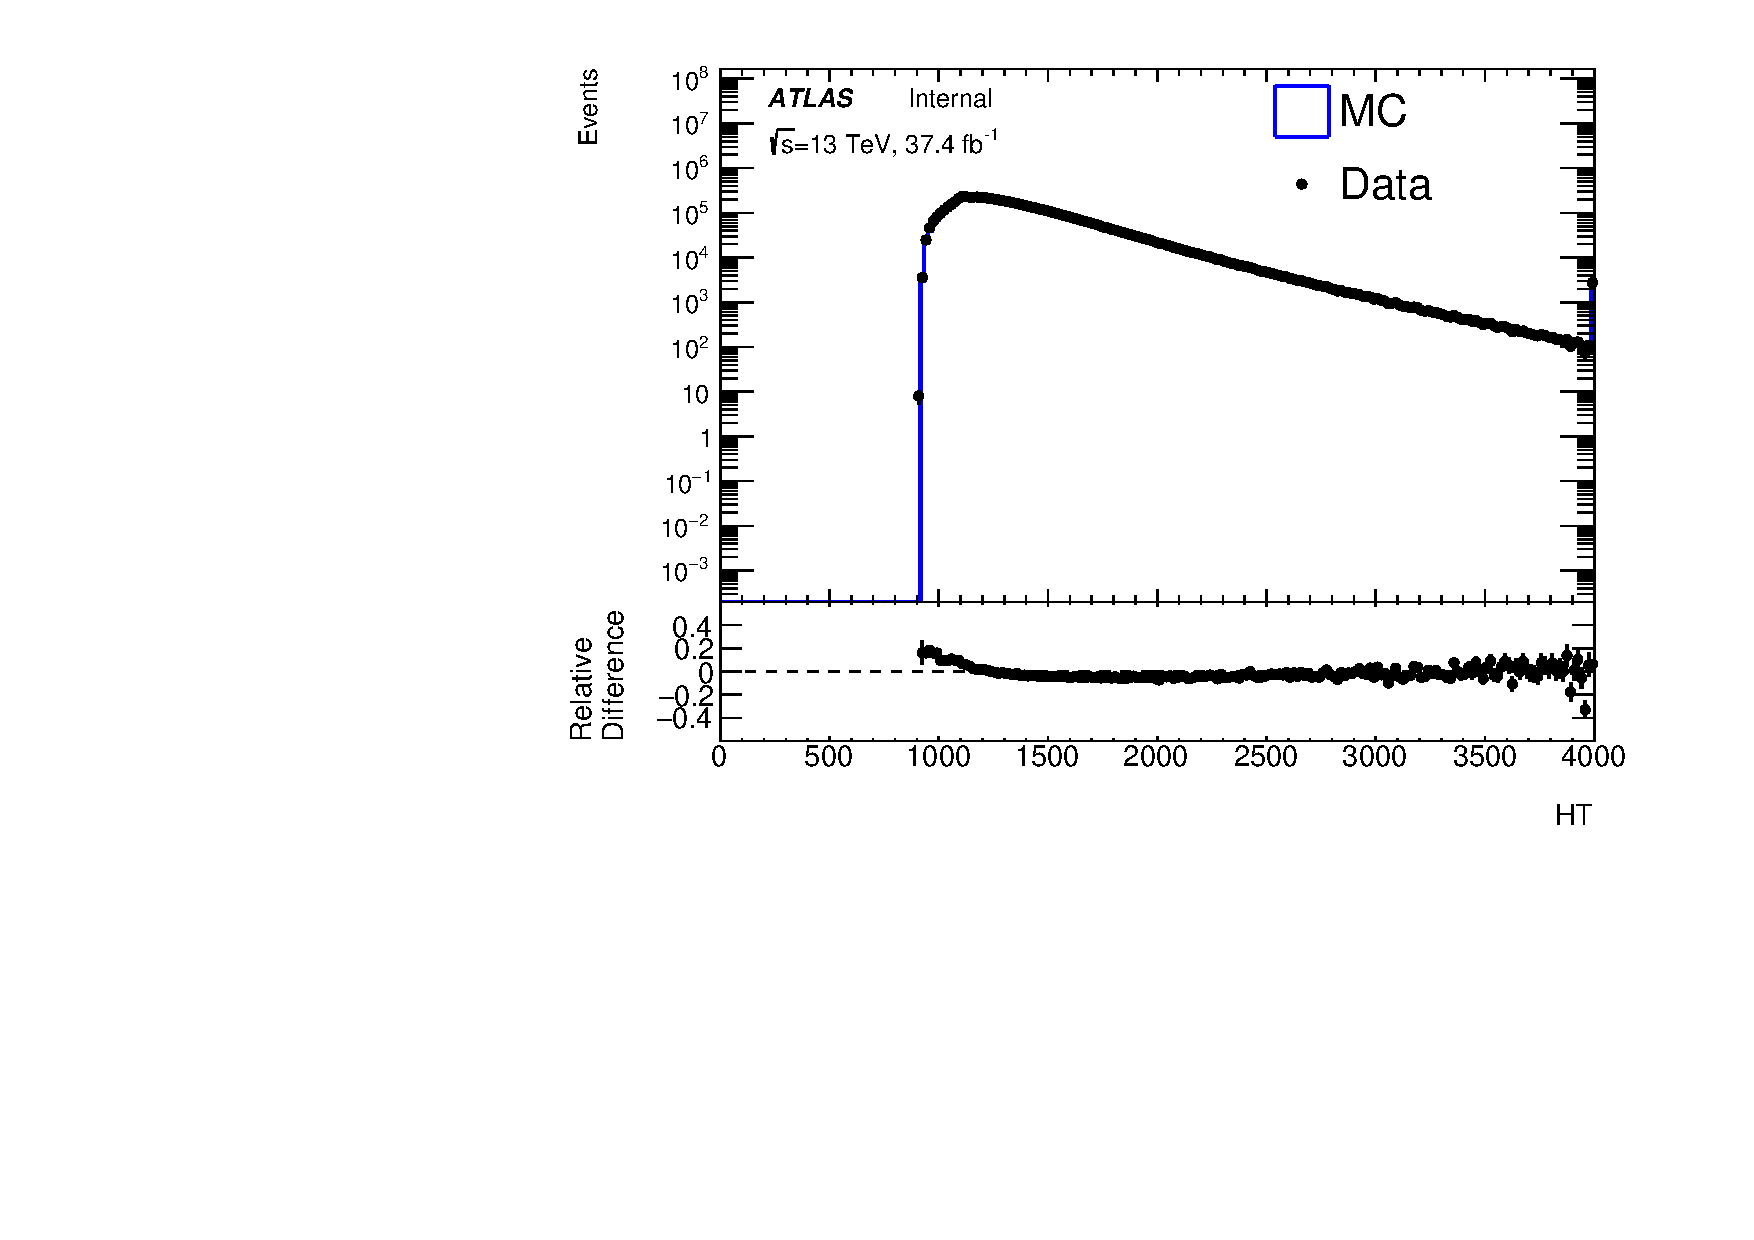
\includegraphics[width=0.45\textwidth]{figures/monitoring/resonant/Moriond_2017/newStudy_HT_logY.pdf}}
% \subfigure[] {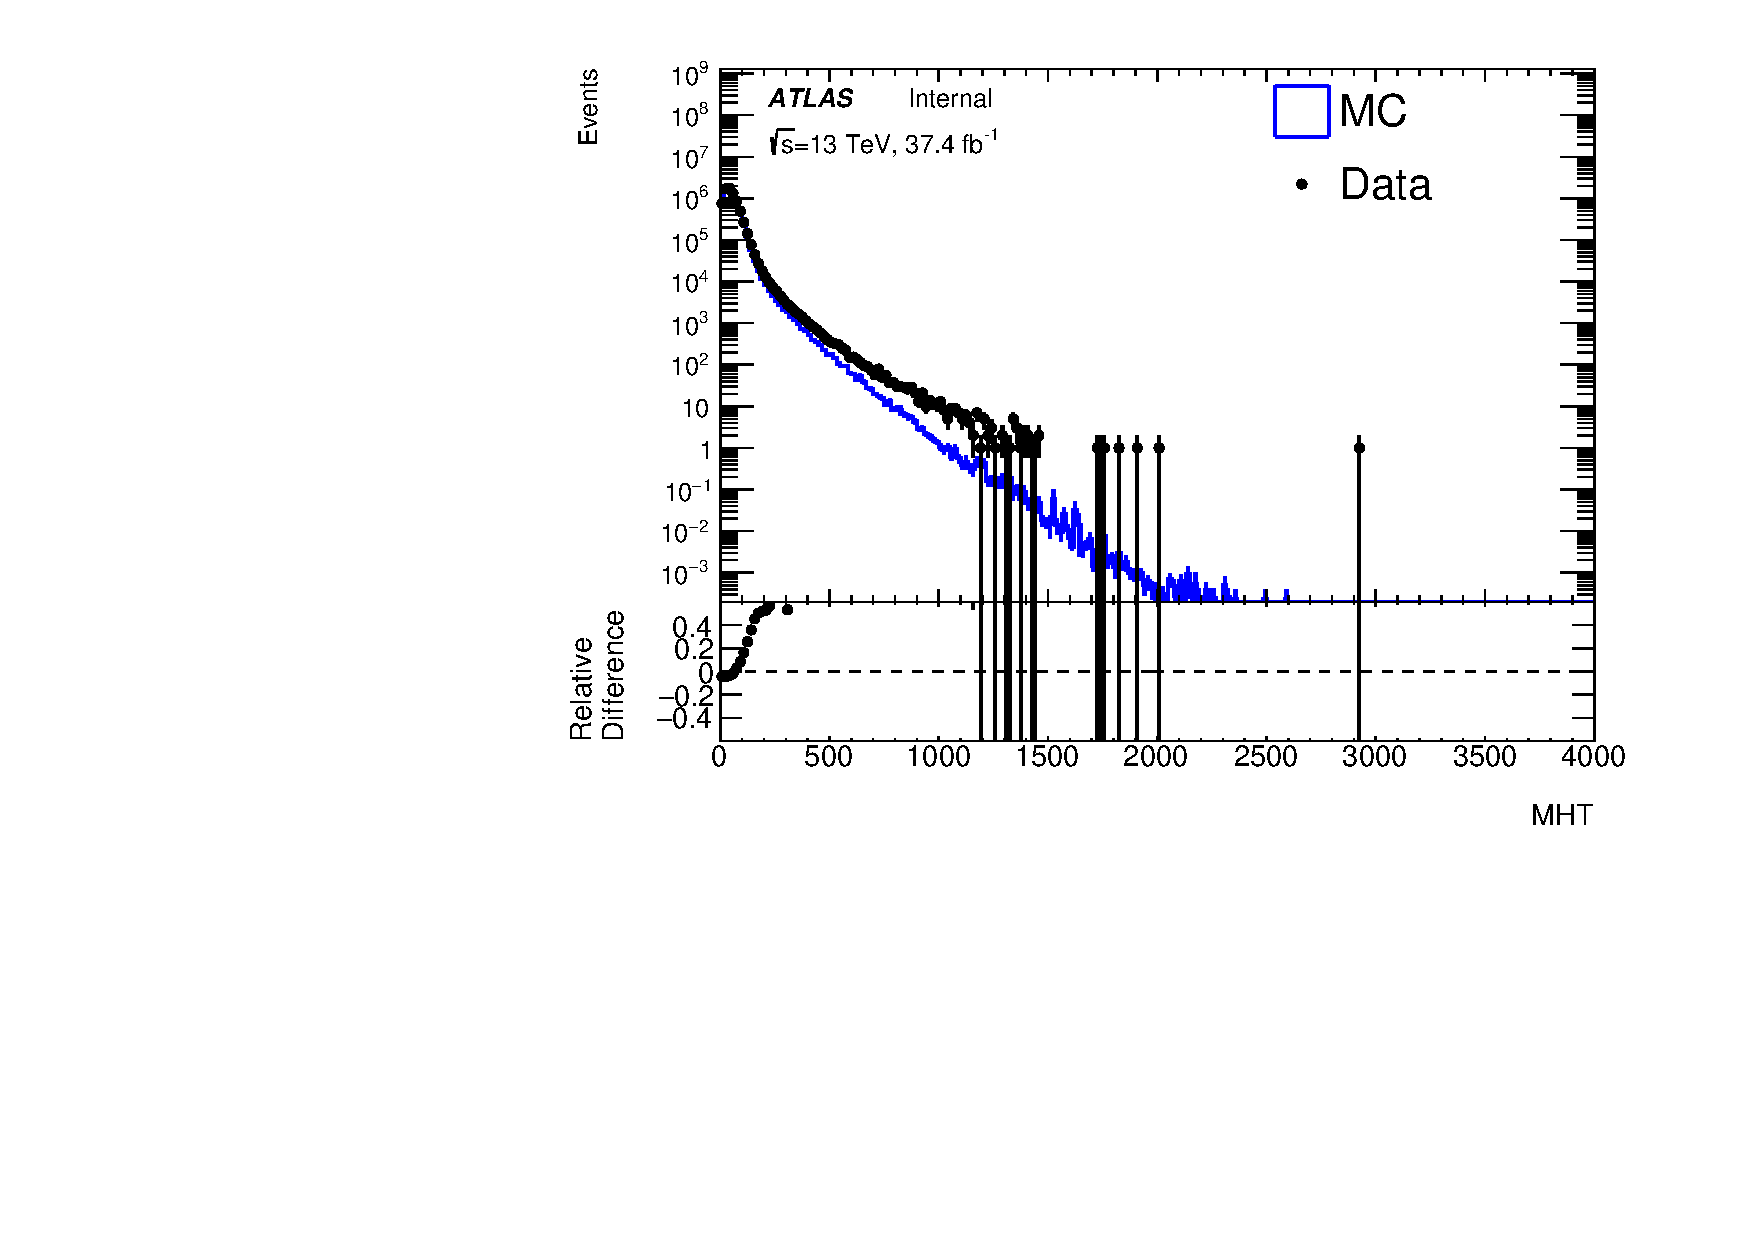
\includegraphics[width=0.45\textwidth]{figures/monitoring/resonant/Moriond_2017/newStudy_MHT_logY.pdf}}
% %
% \subfigure[] {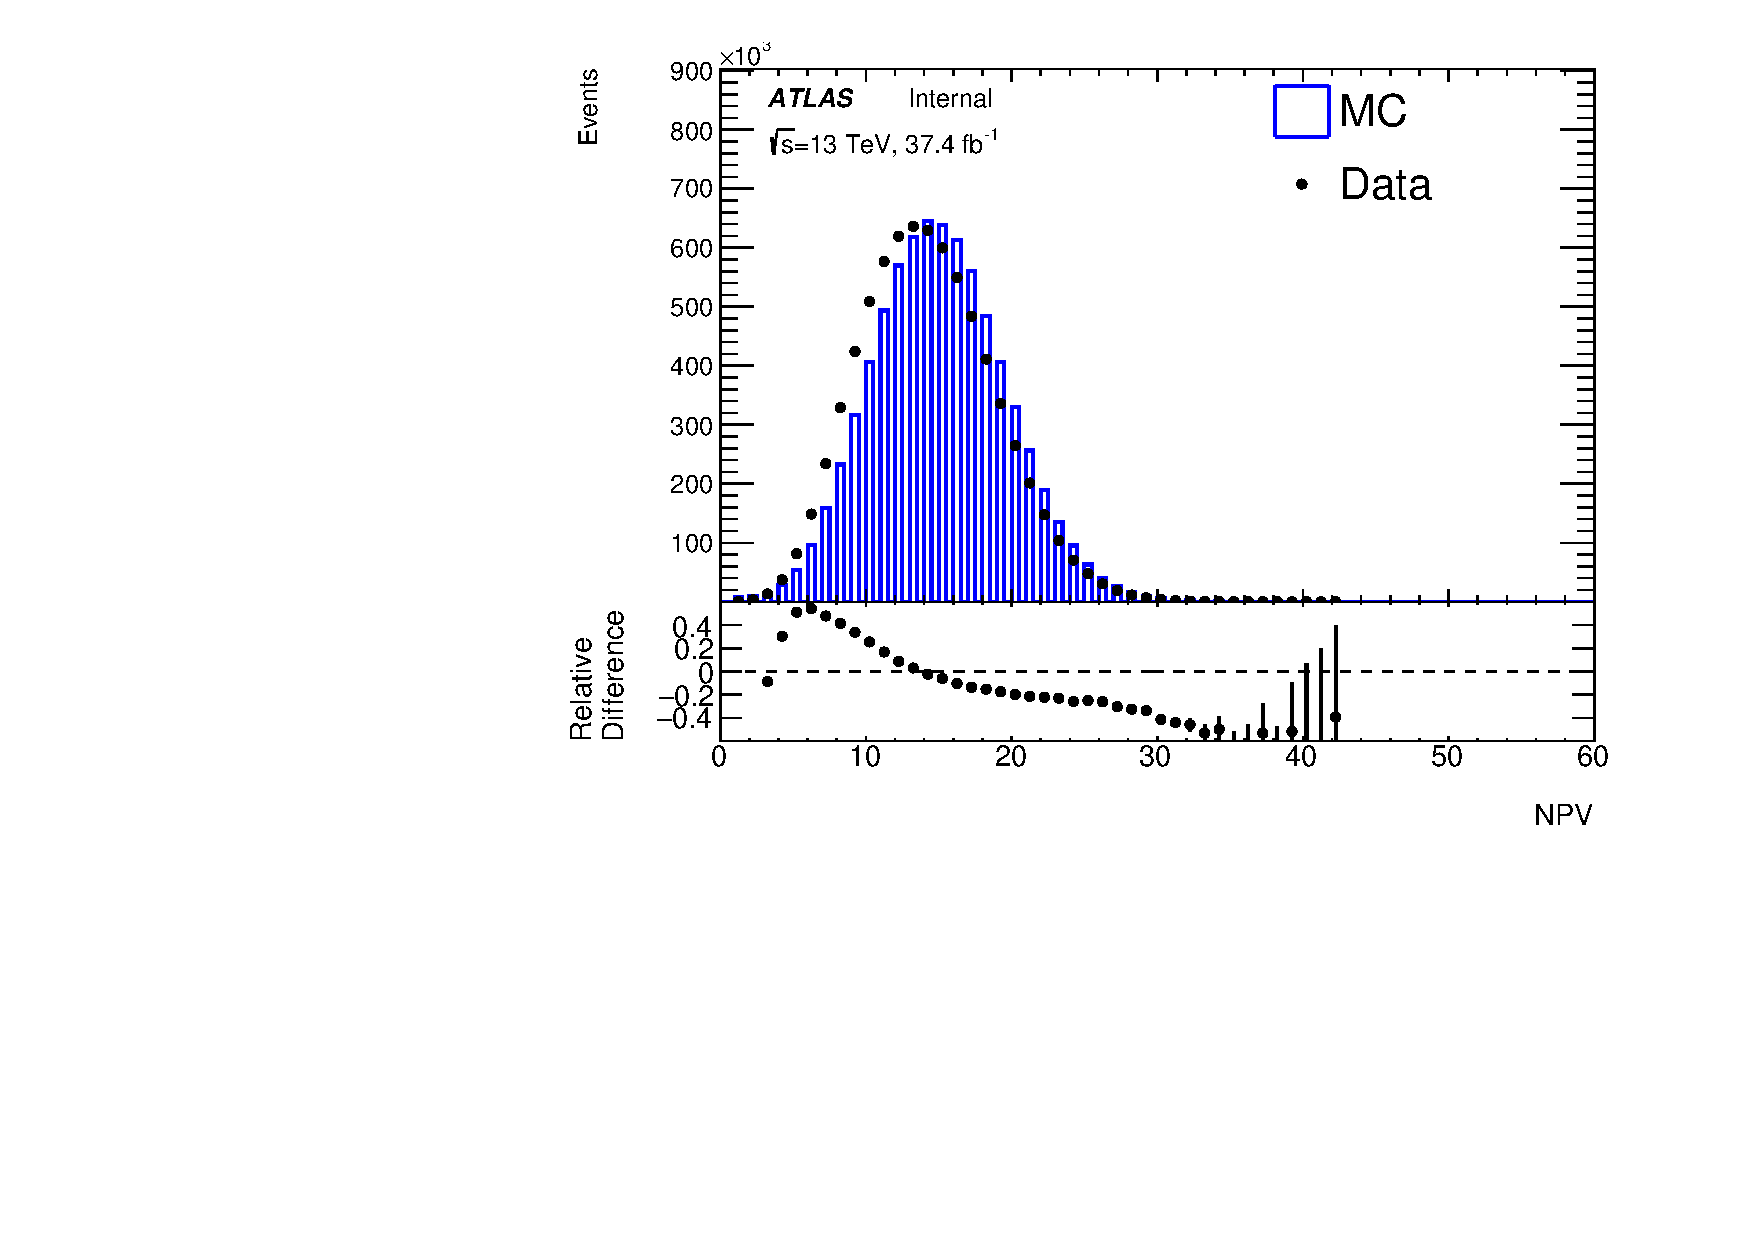
\includegraphics[width=0.45\textwidth]{figures/monitoring/resonant/Moriond_2017/newStudy_NPV.pdf}}
% \subfigure[] {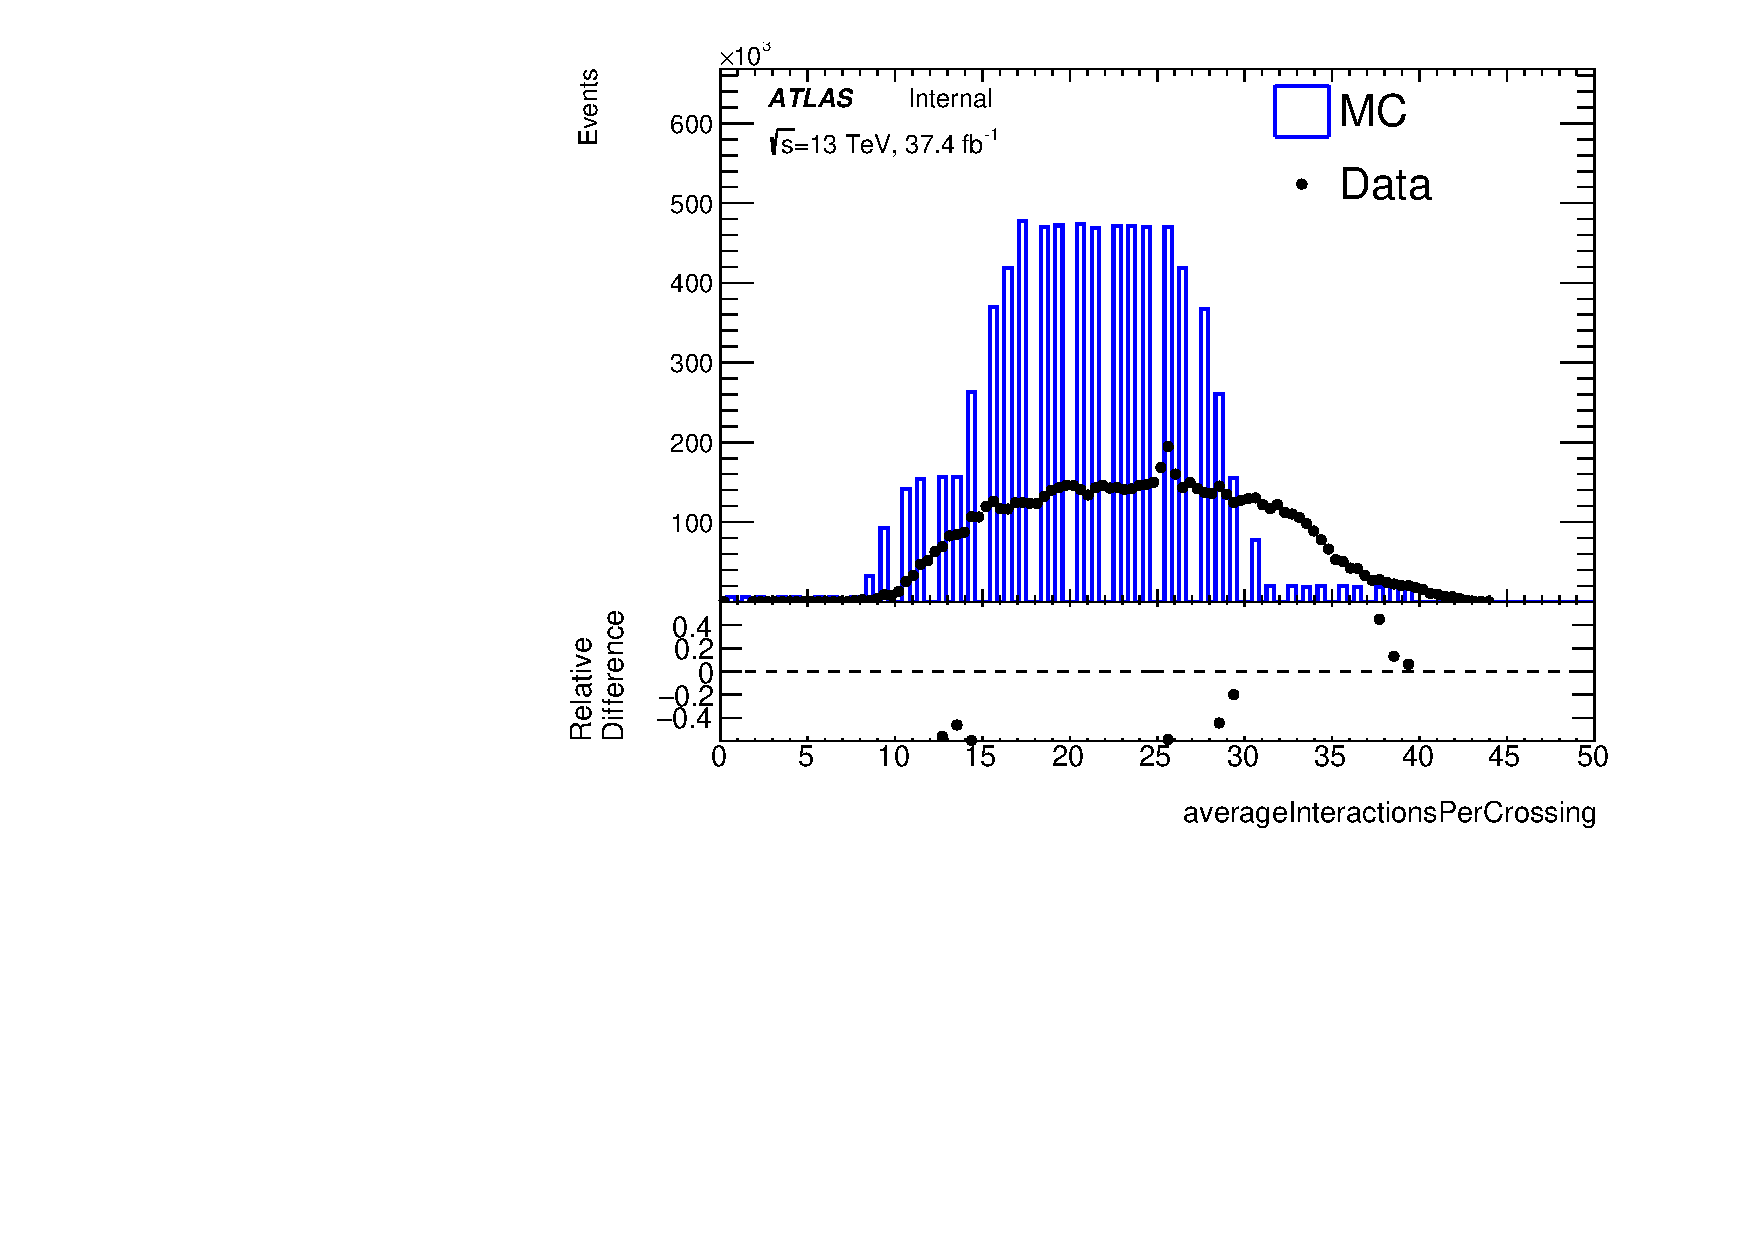
\includegraphics[width=0.45\textwidth]{figures/monitoring/resonant/Moriond_2017/newStudy_averageInteractionsPerCrossing.pdf}}
% \caption{Monitoring plots on %2016 data, 
% the resonant selection. (a) $H_T$, (b) $MH_T$ (missing transverse momentum calculated only from the jets in the event), (c) number of primary interaction vertices and (d) average interactions per bunch crossing.}
% \label{fig:monitoring1}
%\end{figure}
%
%
%\clearpage

In this section a selection of kinematic and monitoring plots produced with the resonant selection on the complete resonance dataset is shown 
(Figures~\ref{fig:JJmonitoring1},  
\ref{fig:JJmonitoring5}, \ref{fig:JJmonitoring6}). These plots are relative to \integLumi of data collected in 2015 and 2016.
 GRL has been applied here.


\begin{figure}[htb]
 \centering
 \subfigure[] {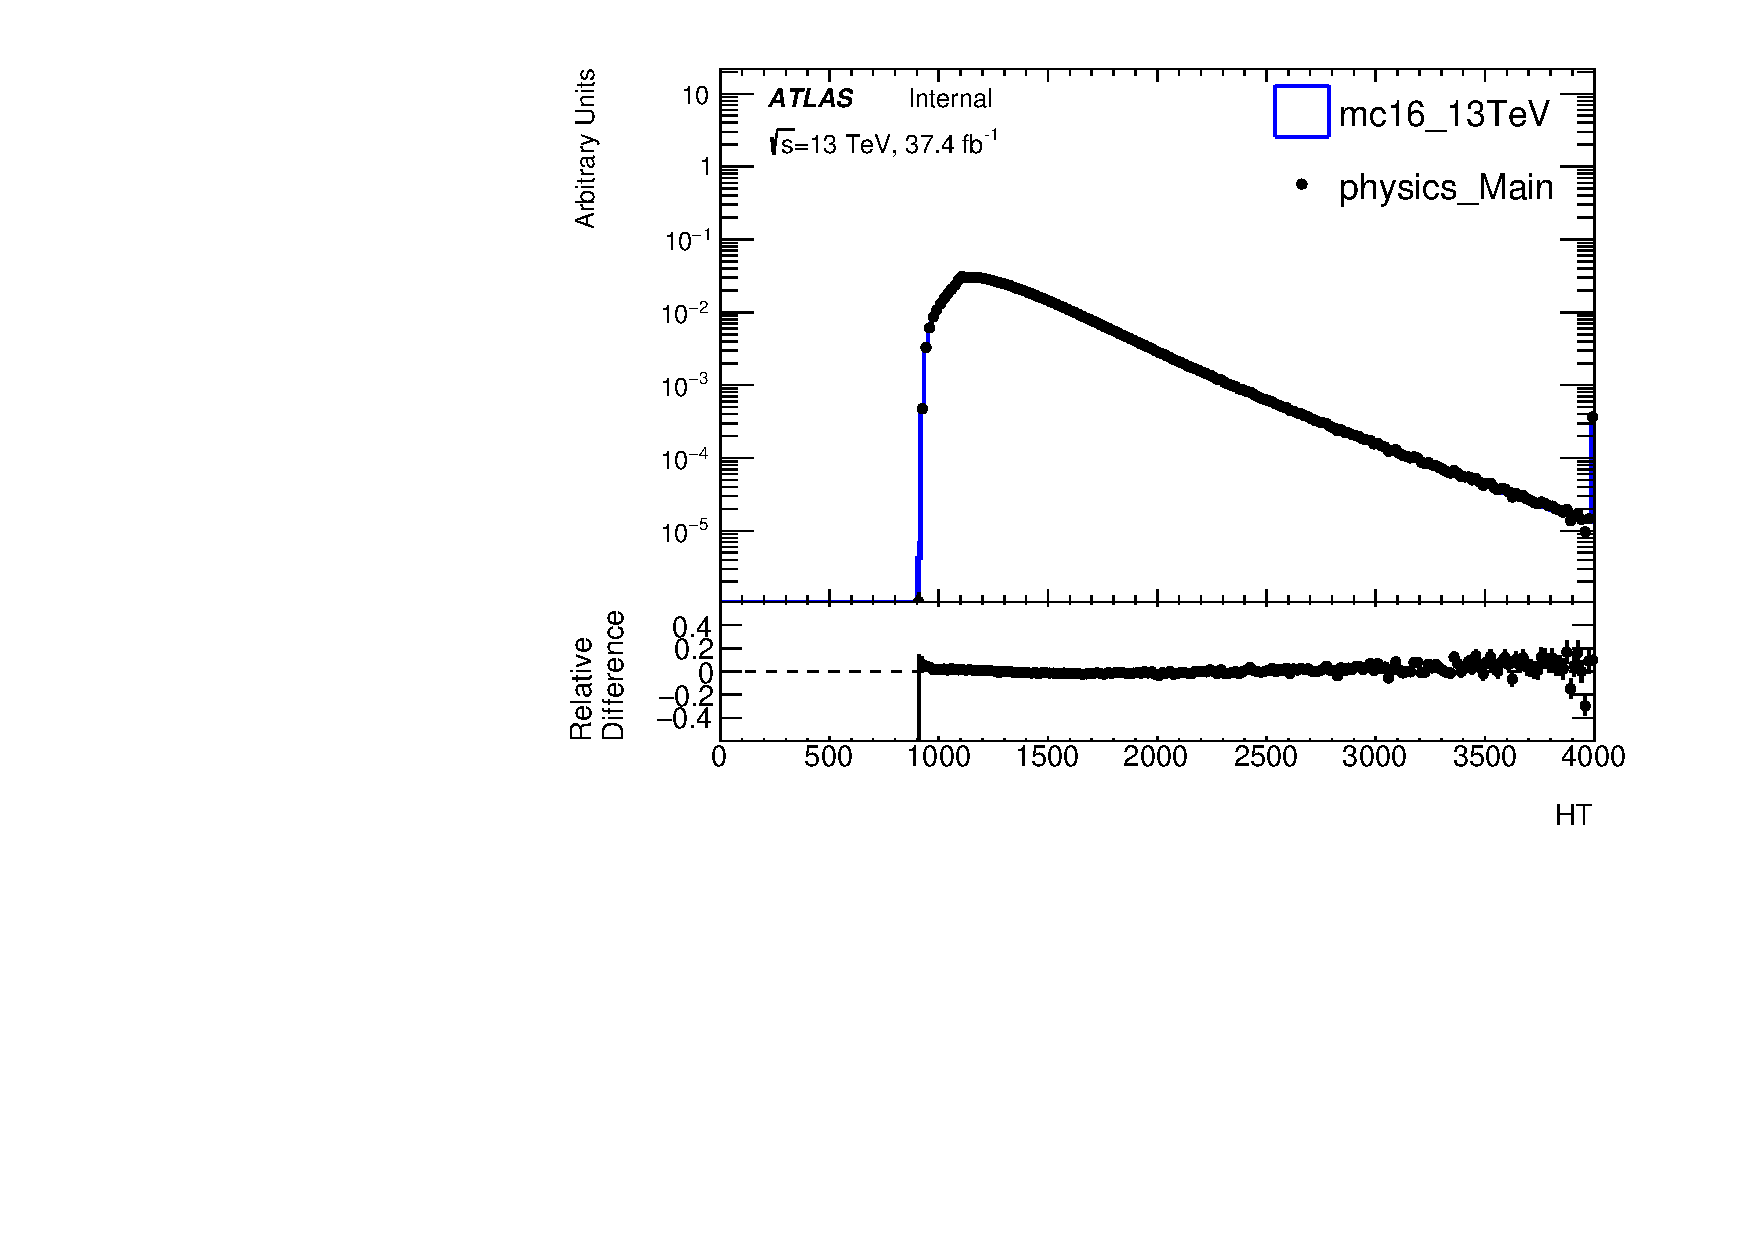
\includegraphics[width=0.45\textwidth]{figures/monitoring/resonant/2015-16/JJ/newStudy_HT_logY_JJv01.pdf}}
 \subfigure[] {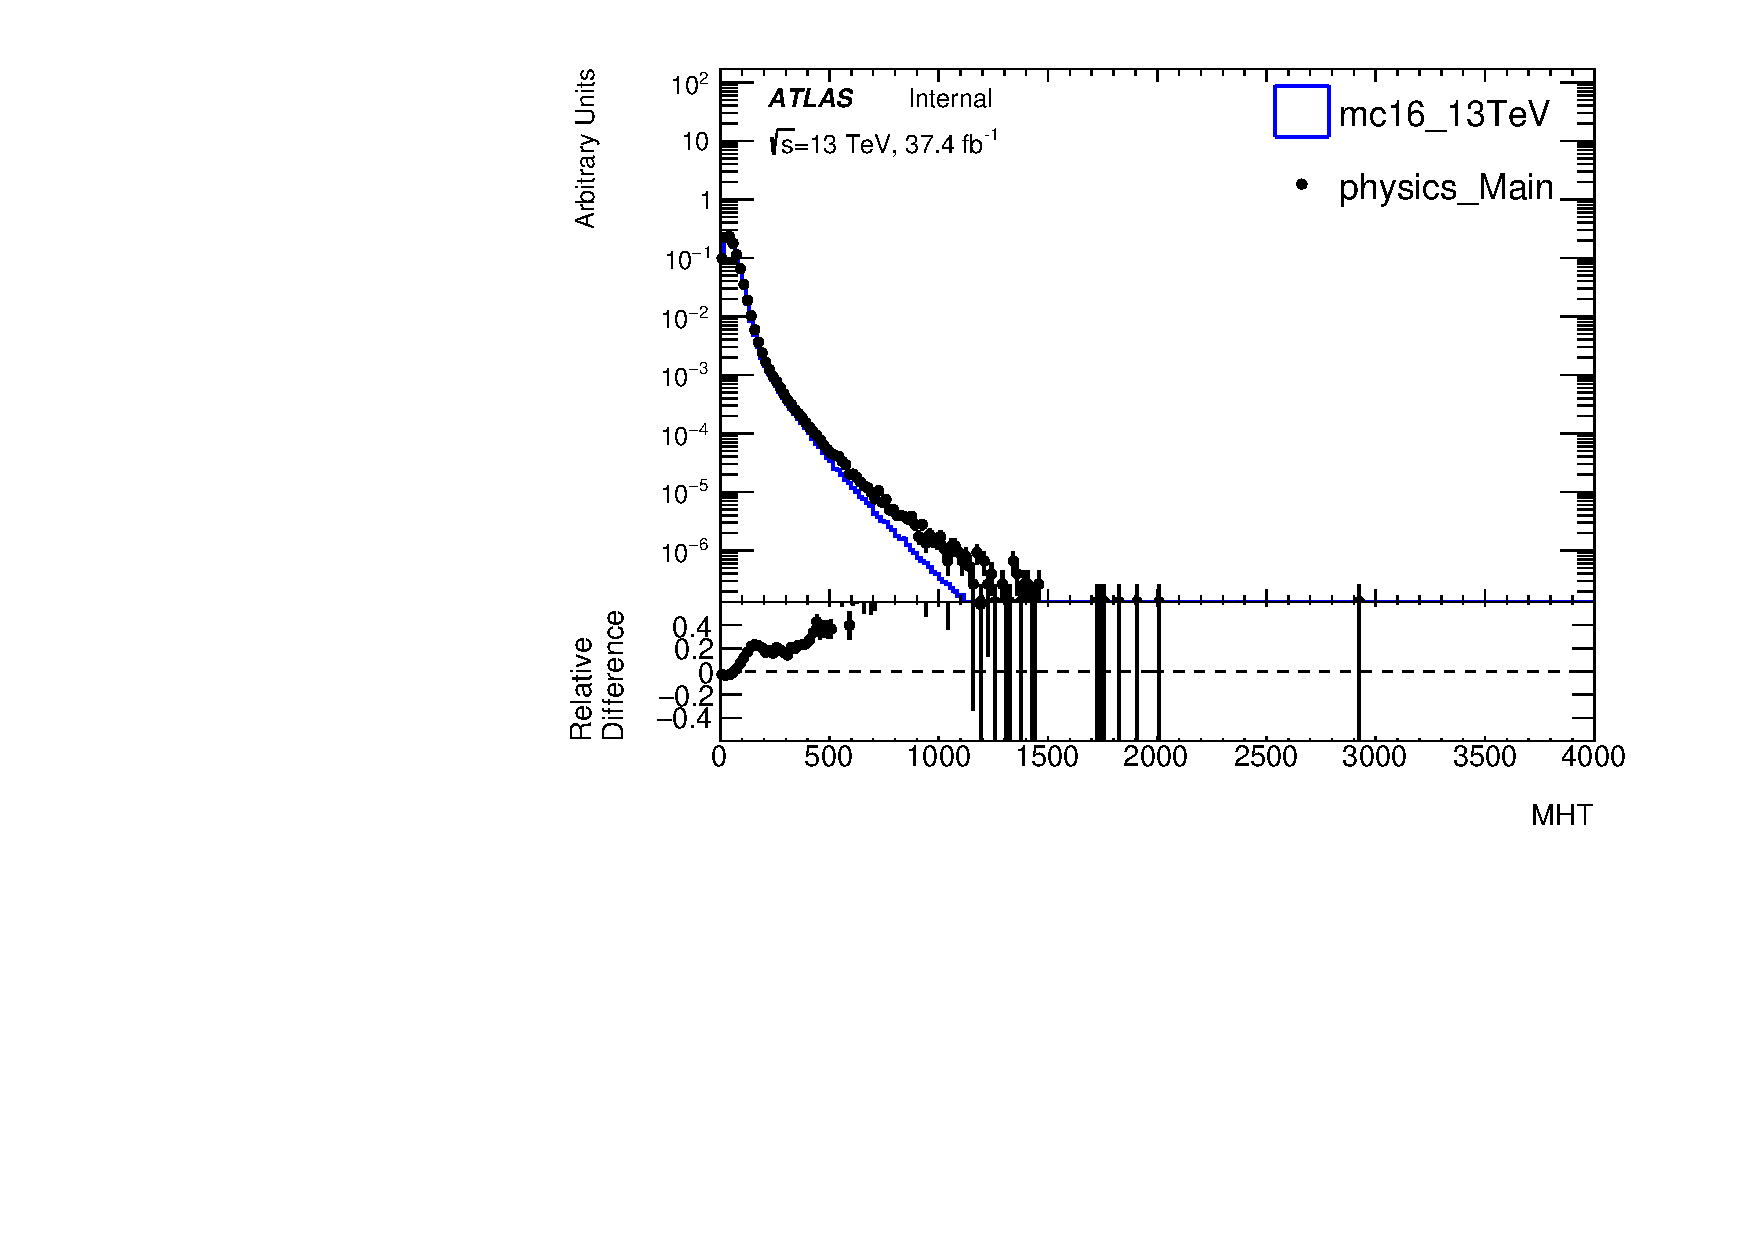
\includegraphics[width=0.45\textwidth]{figures/monitoring/resonant/2015-16/JJ/newStudy_MHT_logY_JJv01.pdf}}
 %
 \subfigure[] {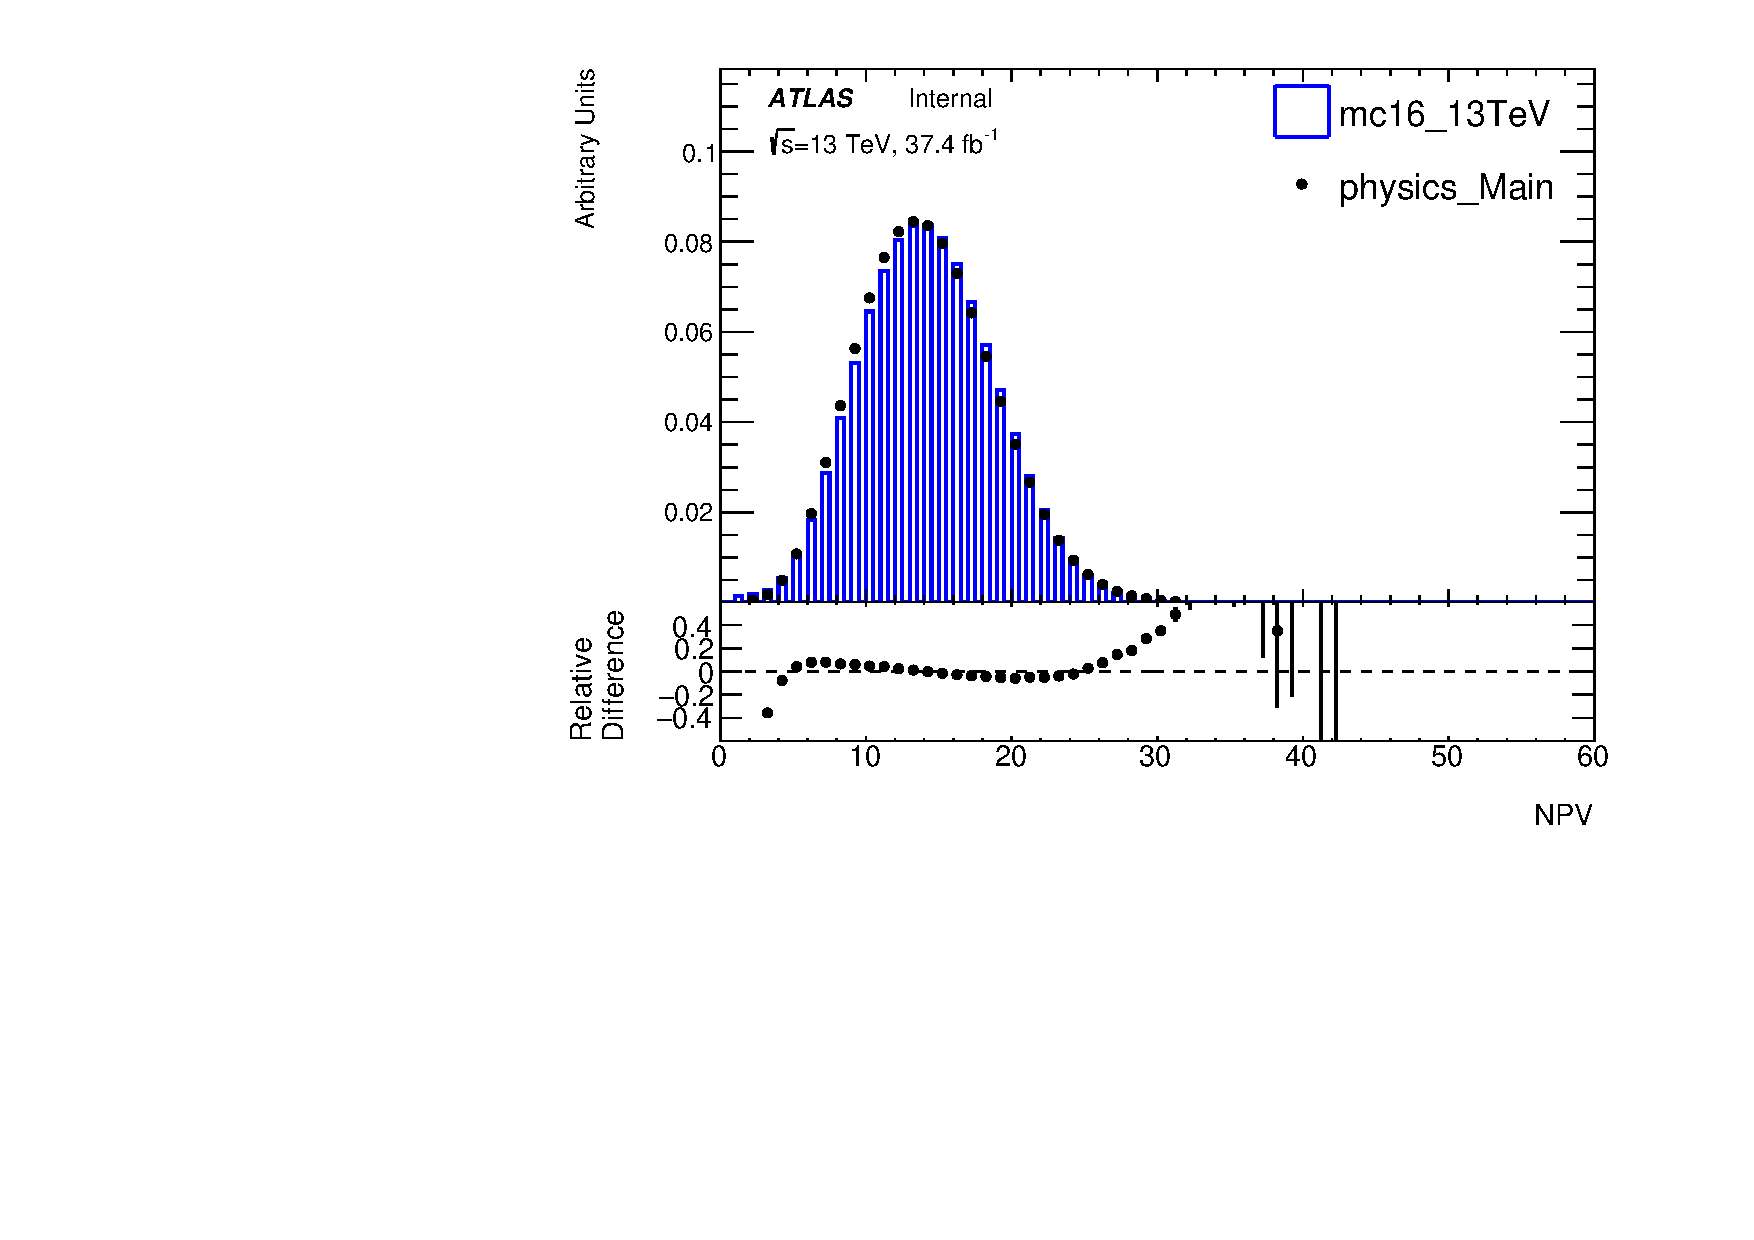
\includegraphics[width=0.45\textwidth]{figures/monitoring/resonant/2015-16/JJ/newStudy_NPV_JJv01.pdf}}
 \subfigure[] {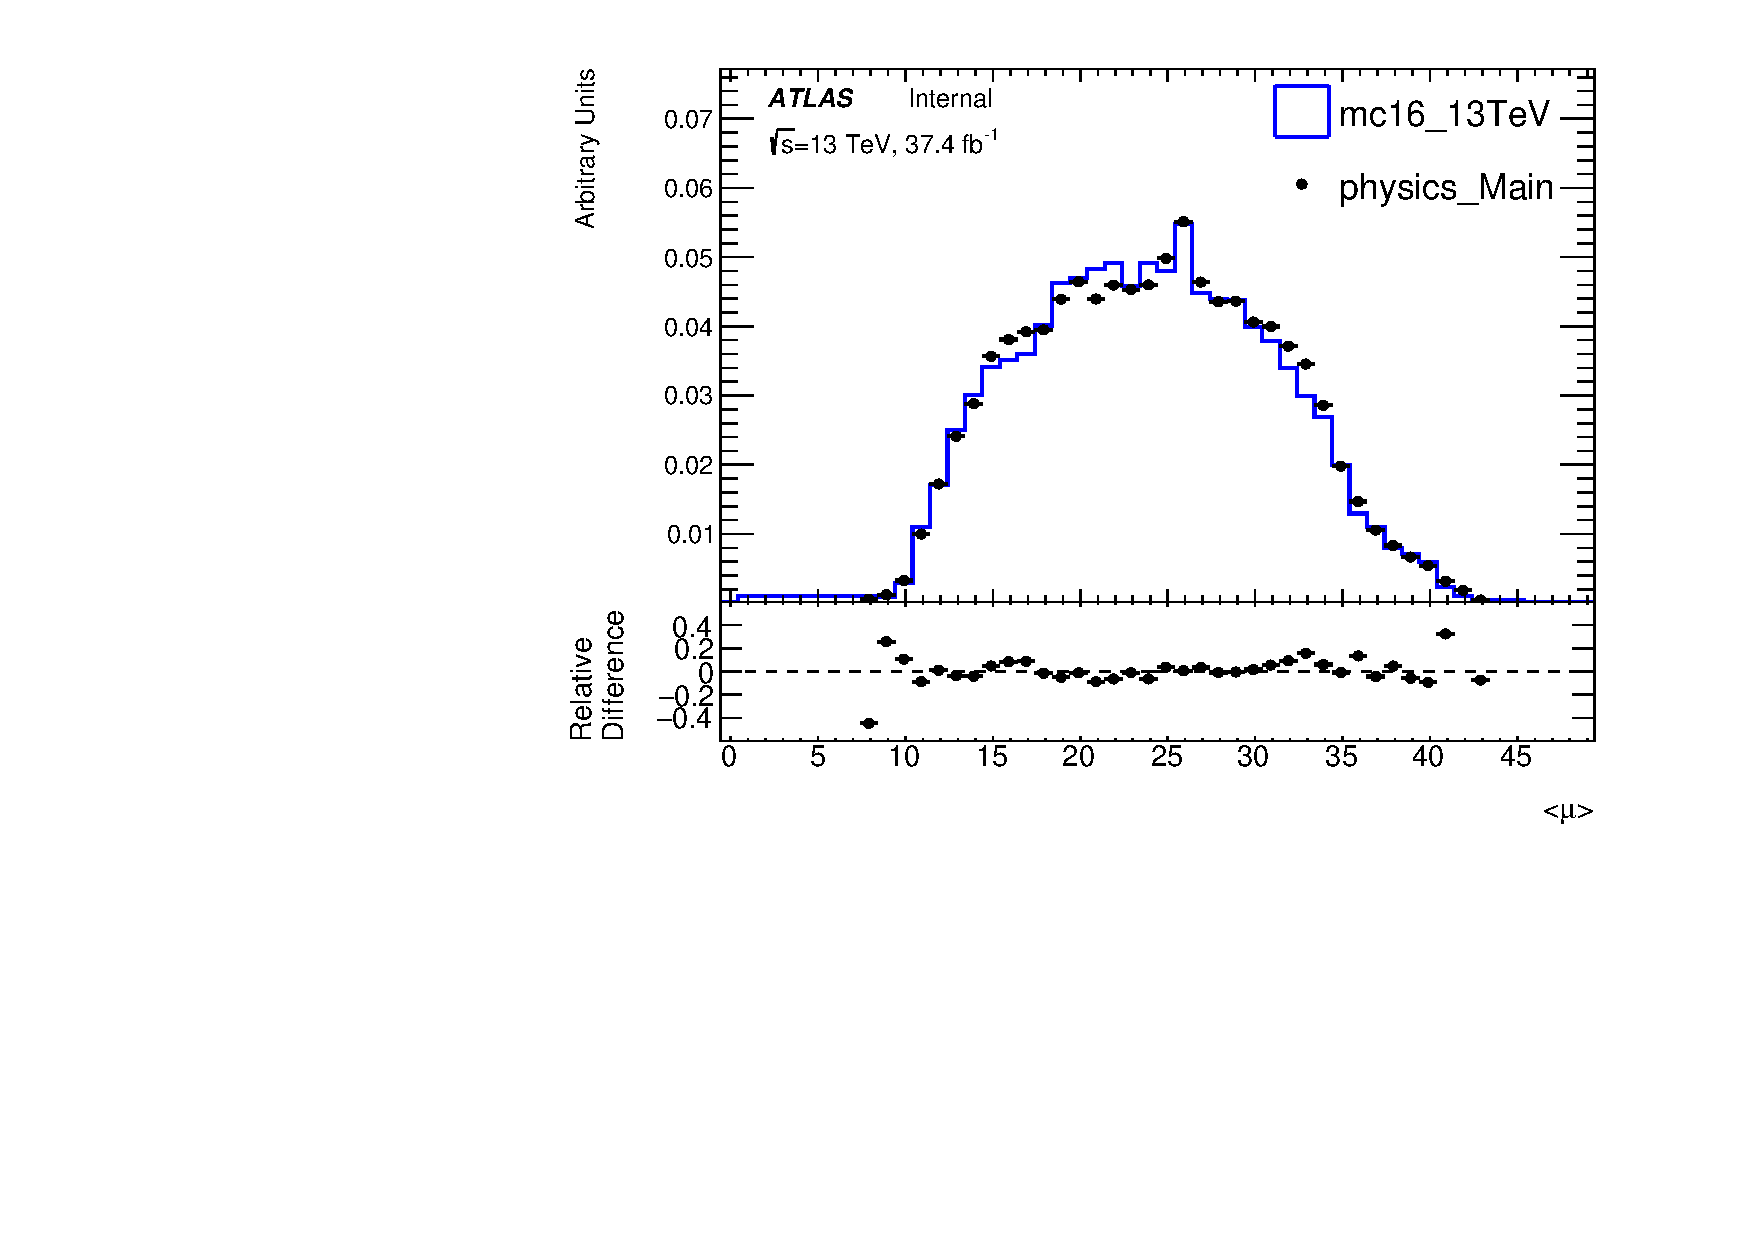
\includegraphics[width=0.45\textwidth]{figures/monitoring/resonant/2015-16/JJ/newStudy_averageInteractionsPerCrossing_JJv01.pdf}}
 %

 \caption{Monitoring plots on %2016 data, 
 the JJ resonant selection. (a) $H_T$, (b) $MH_T$ (missing transverse momentum calculated only from the jets in the event), (c) number of primary interaction vertices and (d) average interactions per bunch crossing.}
 \label{fig:JJmonitoring1}
\end{figure}

 \begin{figure}[htb]
 \centering
  %
 \subfigure[] {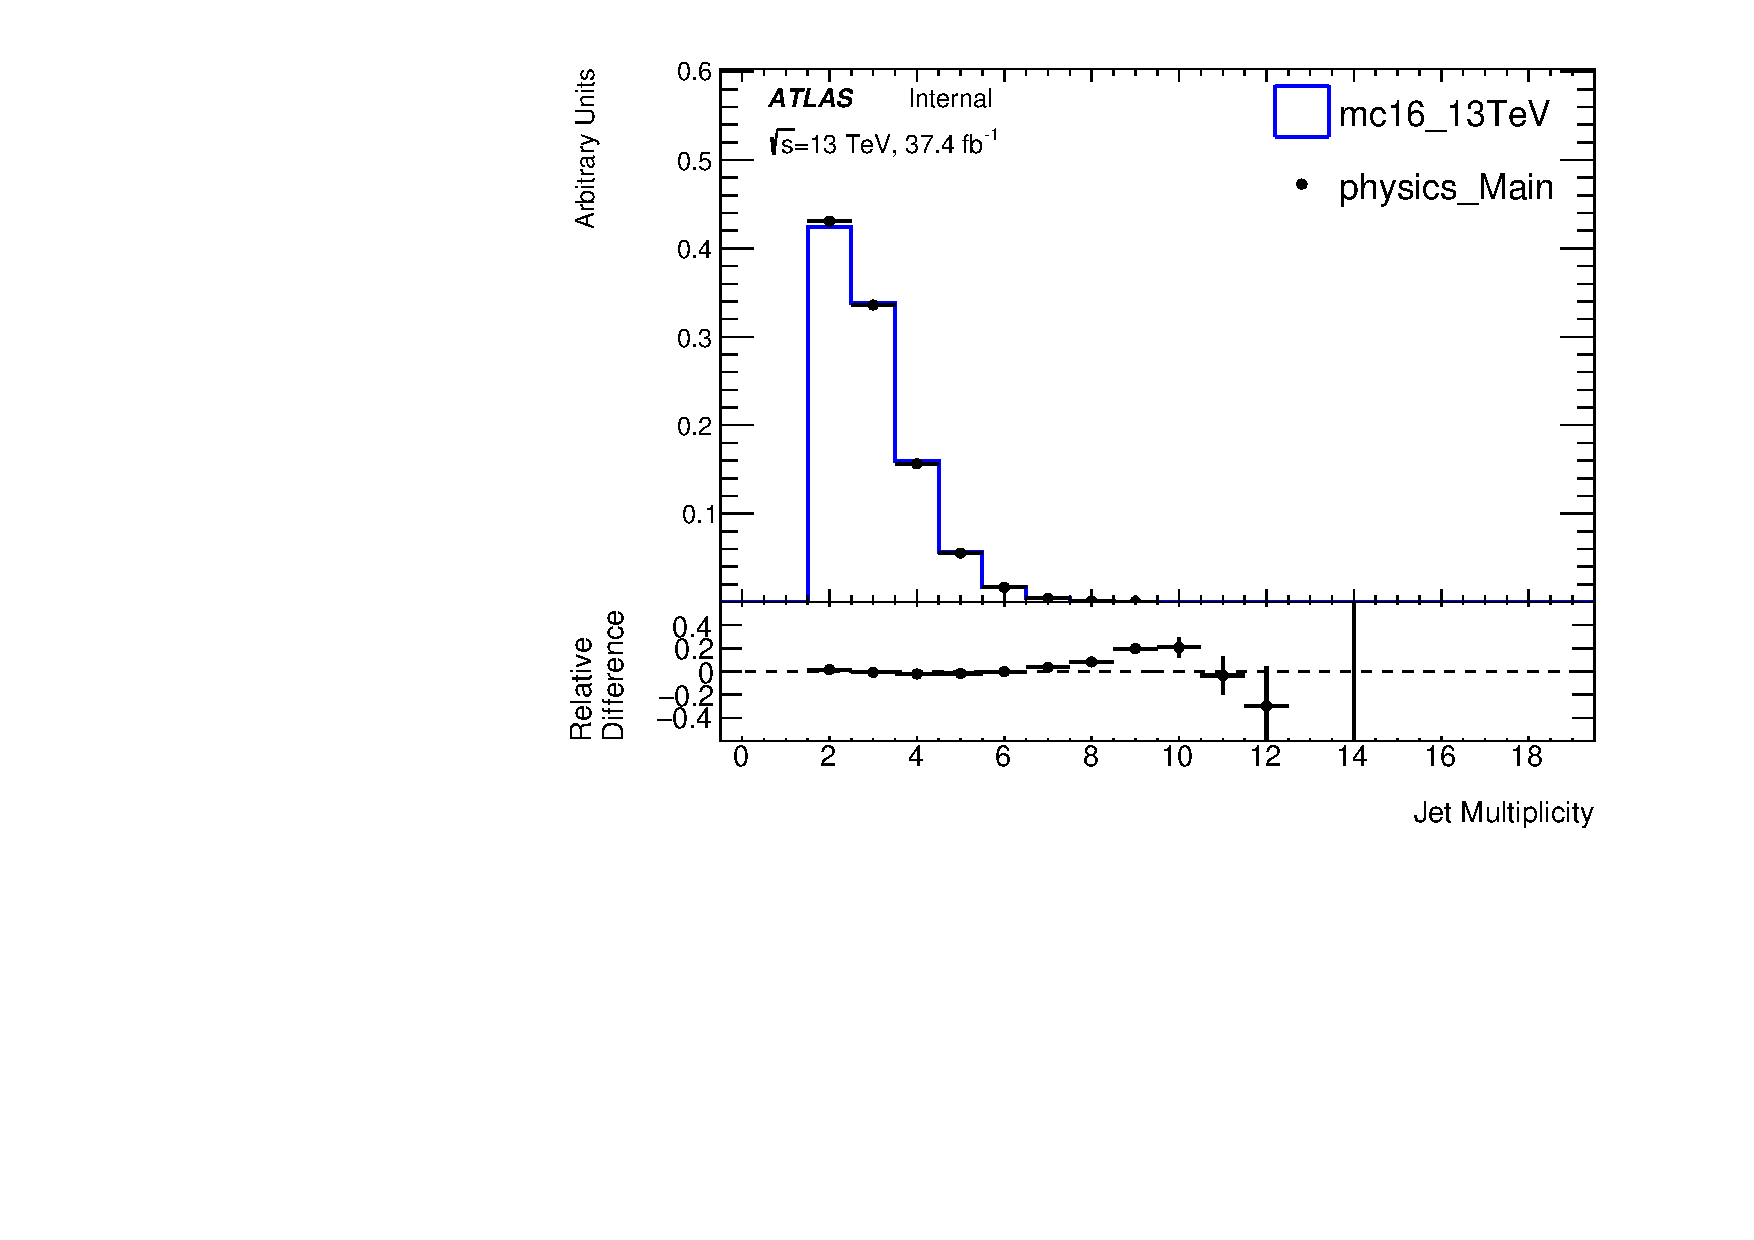
\includegraphics[width=0.45\textwidth]{figures/monitoring/resonant/2015-16/JJ/newStudy_njets_JJv01.pdf}}
 \subfigure[] {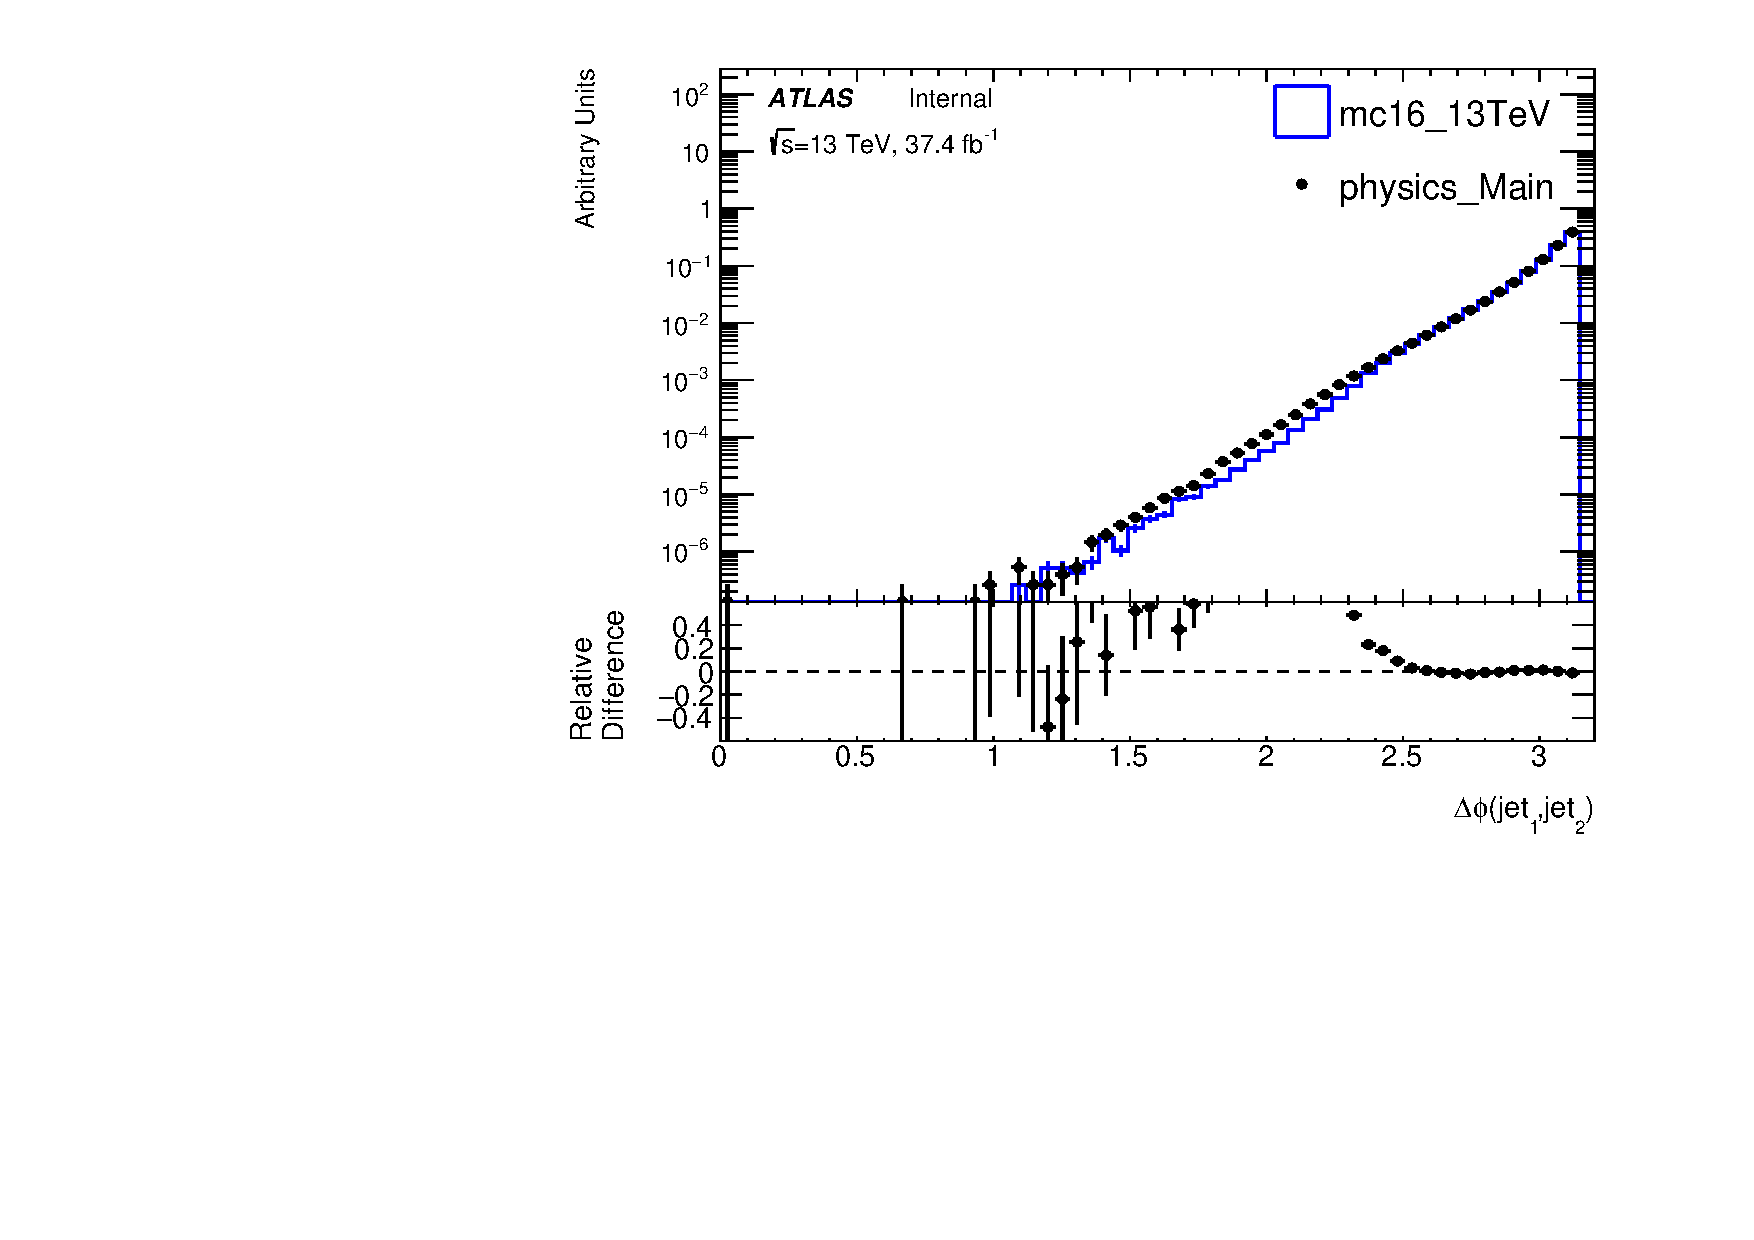
\includegraphics[width=0.45\textwidth]{figures/monitoring/resonant/2015-16/JJ//newStudy_deltaPhi_logY_JJv01.pdf}}

%
 \subfigure[] {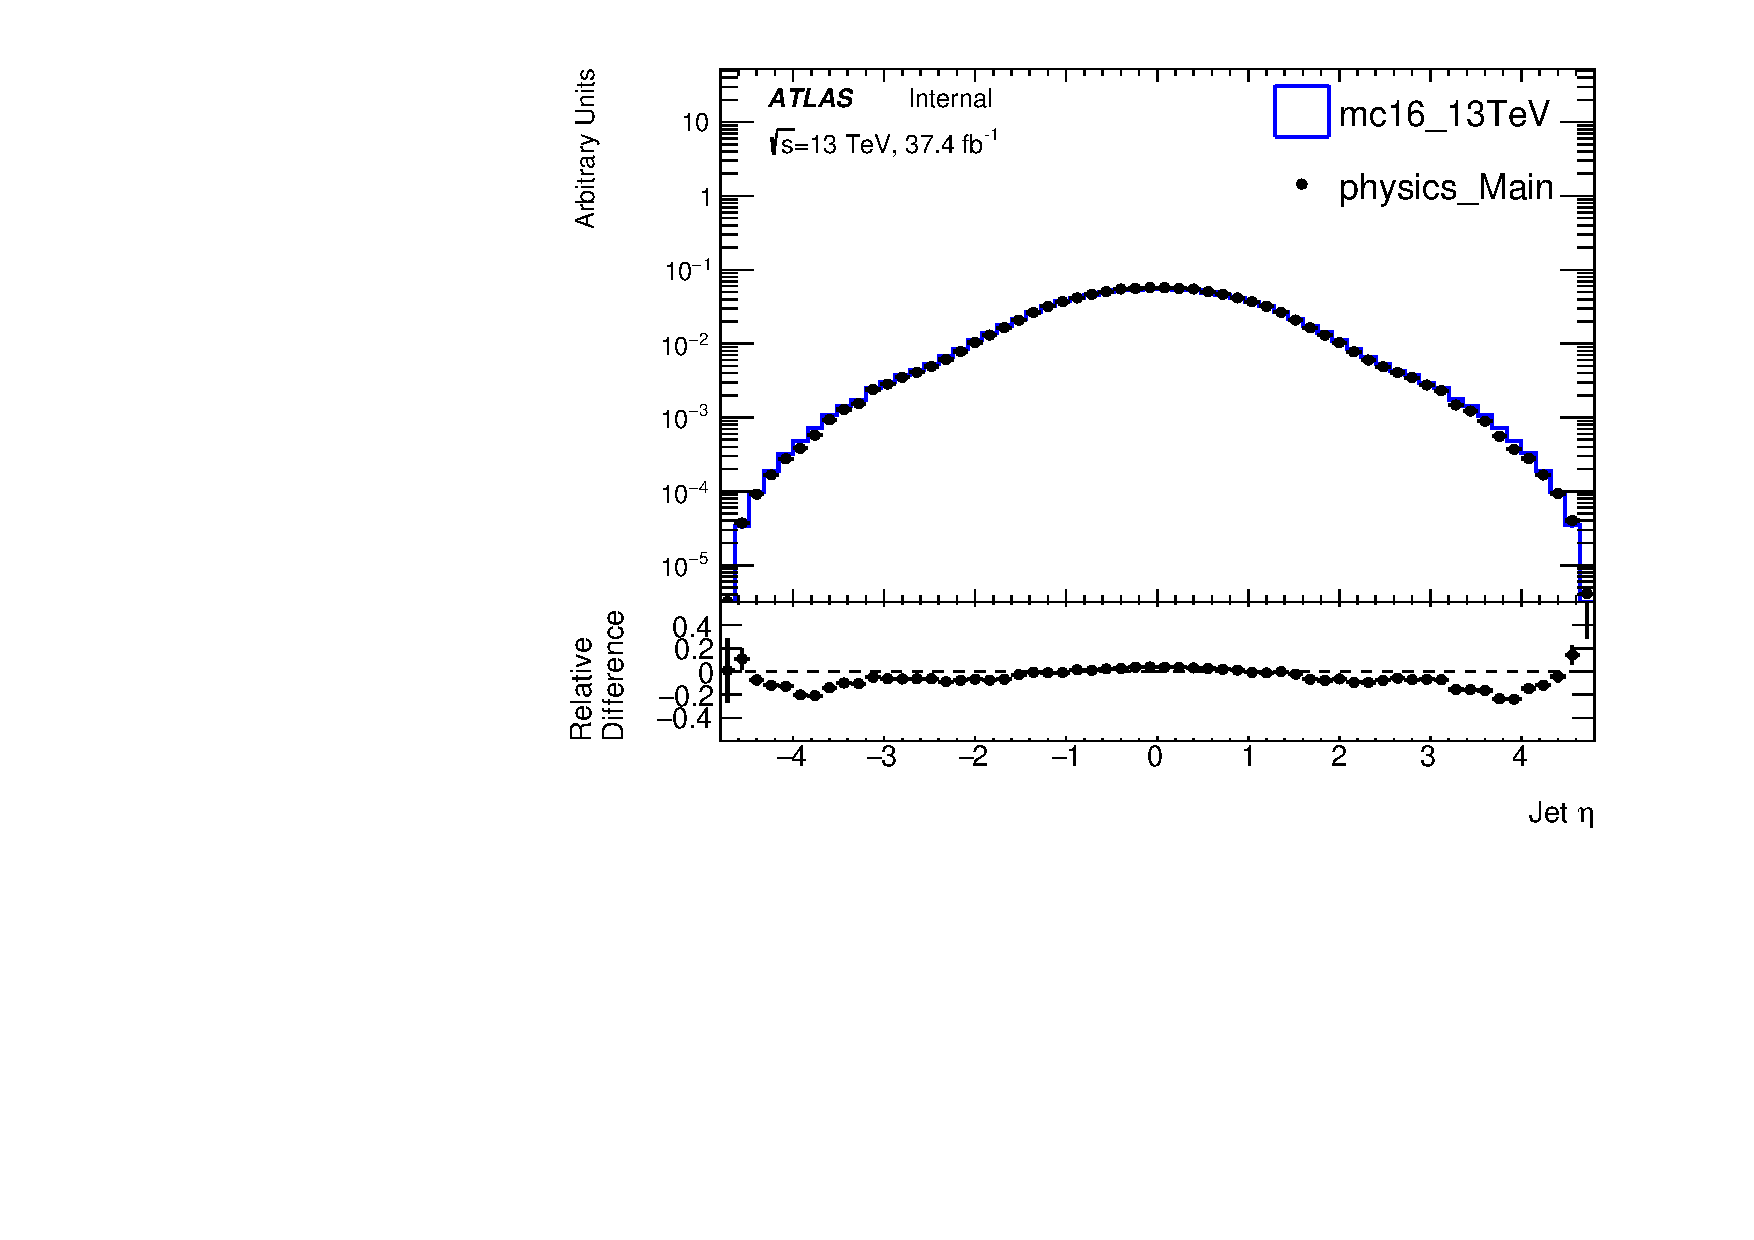
\includegraphics[width=0.45\textwidth]{figures/monitoring/resonant/2015-16/JJ/newStudy_jet_eta_logY_JJv01.pdf}}
 \subfigure[] {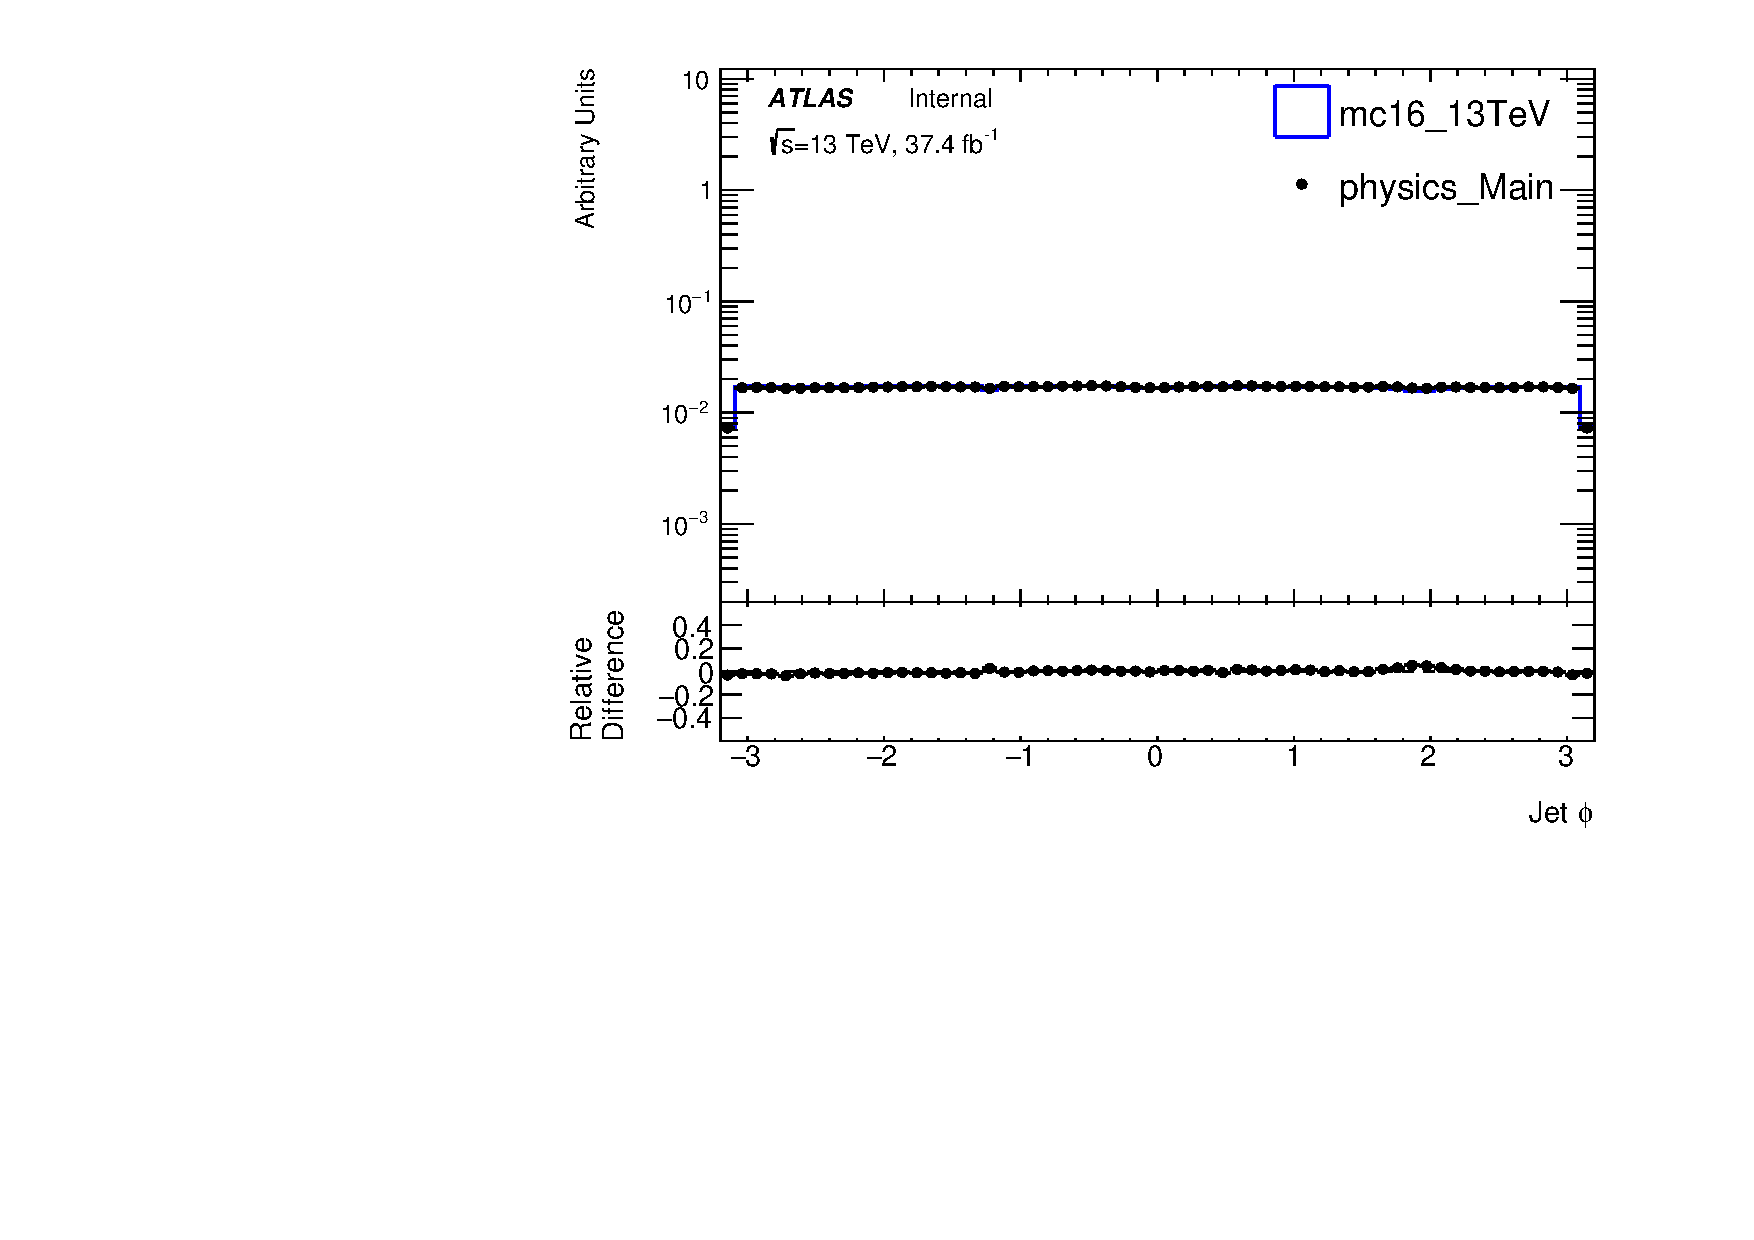
\includegraphics[width=0.45\textwidth]{figures/monitoring/resonant/2015-16/JJ/newStudy_jet_phi_logY_JJv01.pdf}}
 %
 \subfigure[] {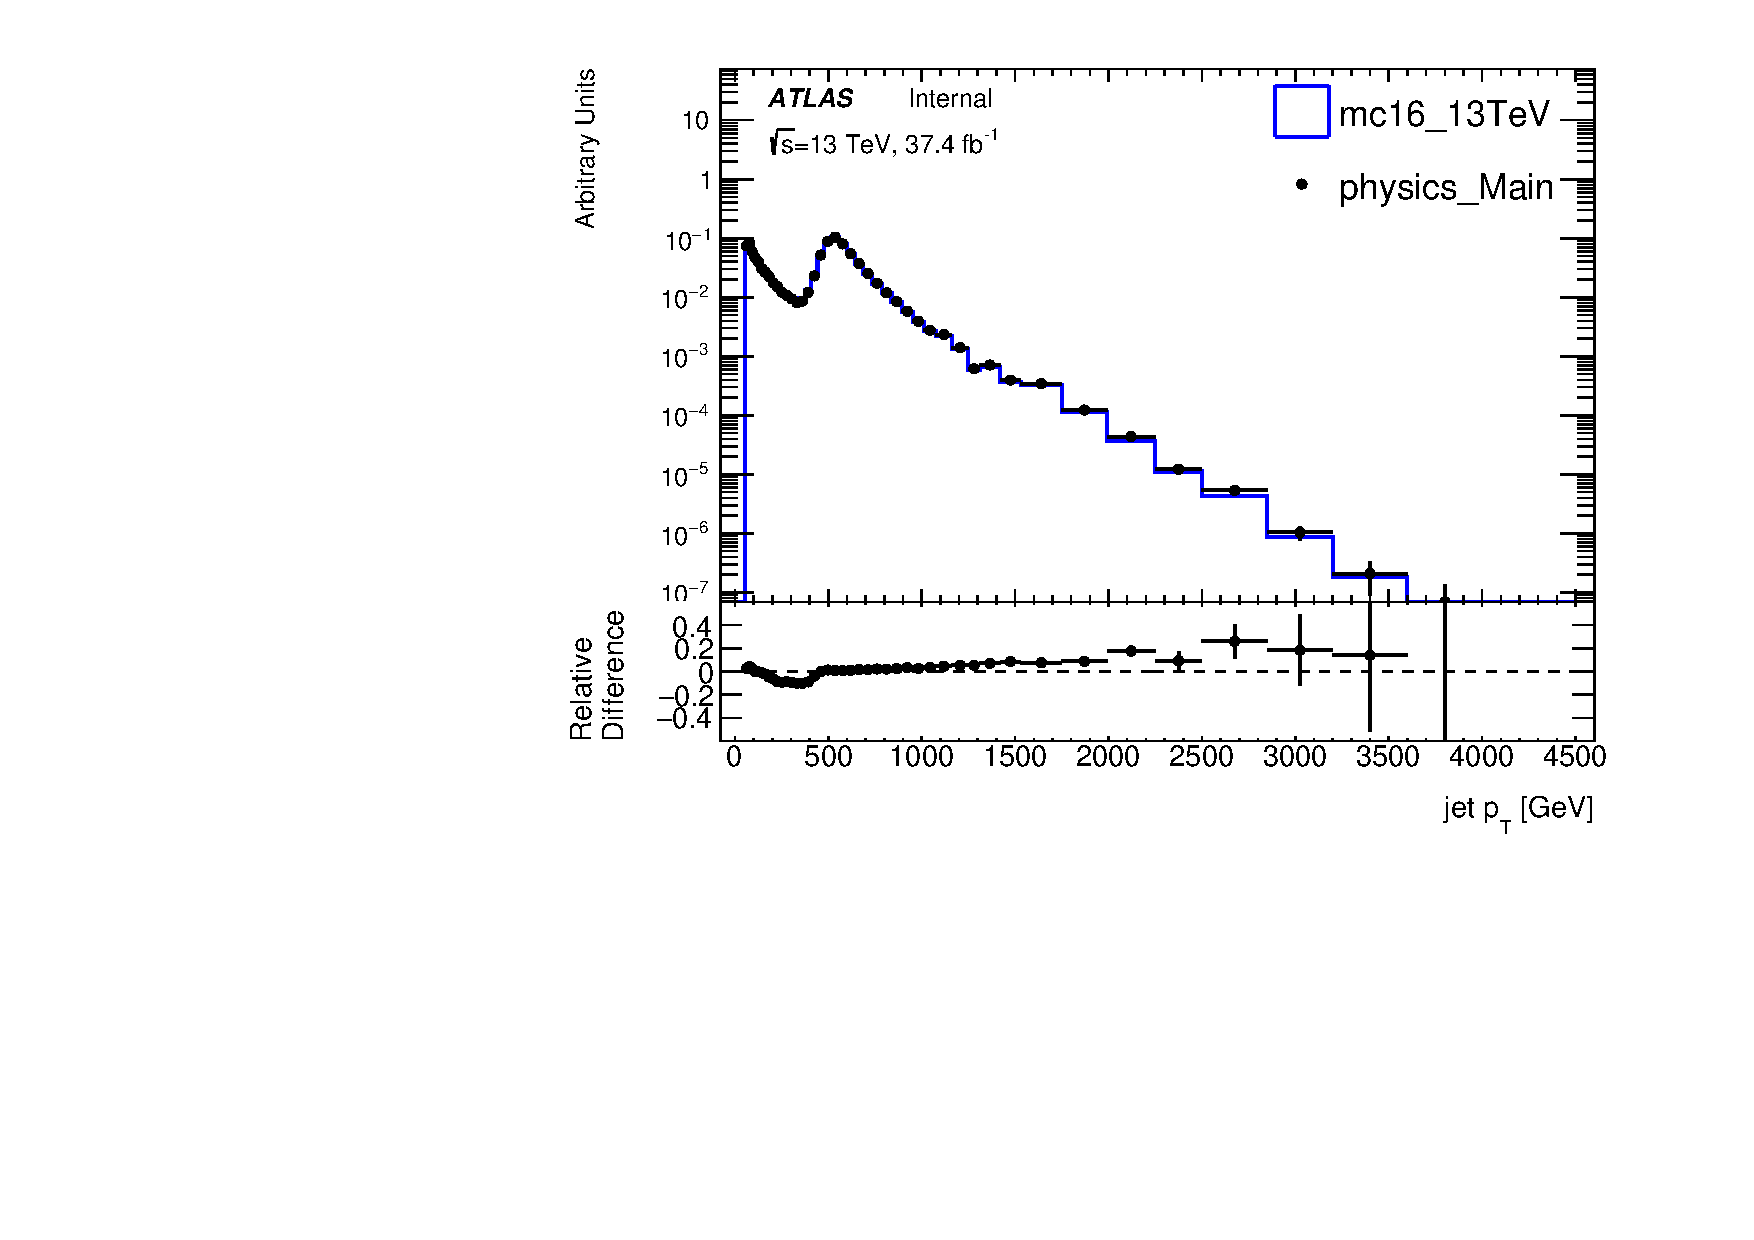
\includegraphics[width=0.45\textwidth]{figures/monitoring/resonant/2015-16/JJ/newStudy_jet_pt_logY_JJv01.pdf}}
 \subfigure[] {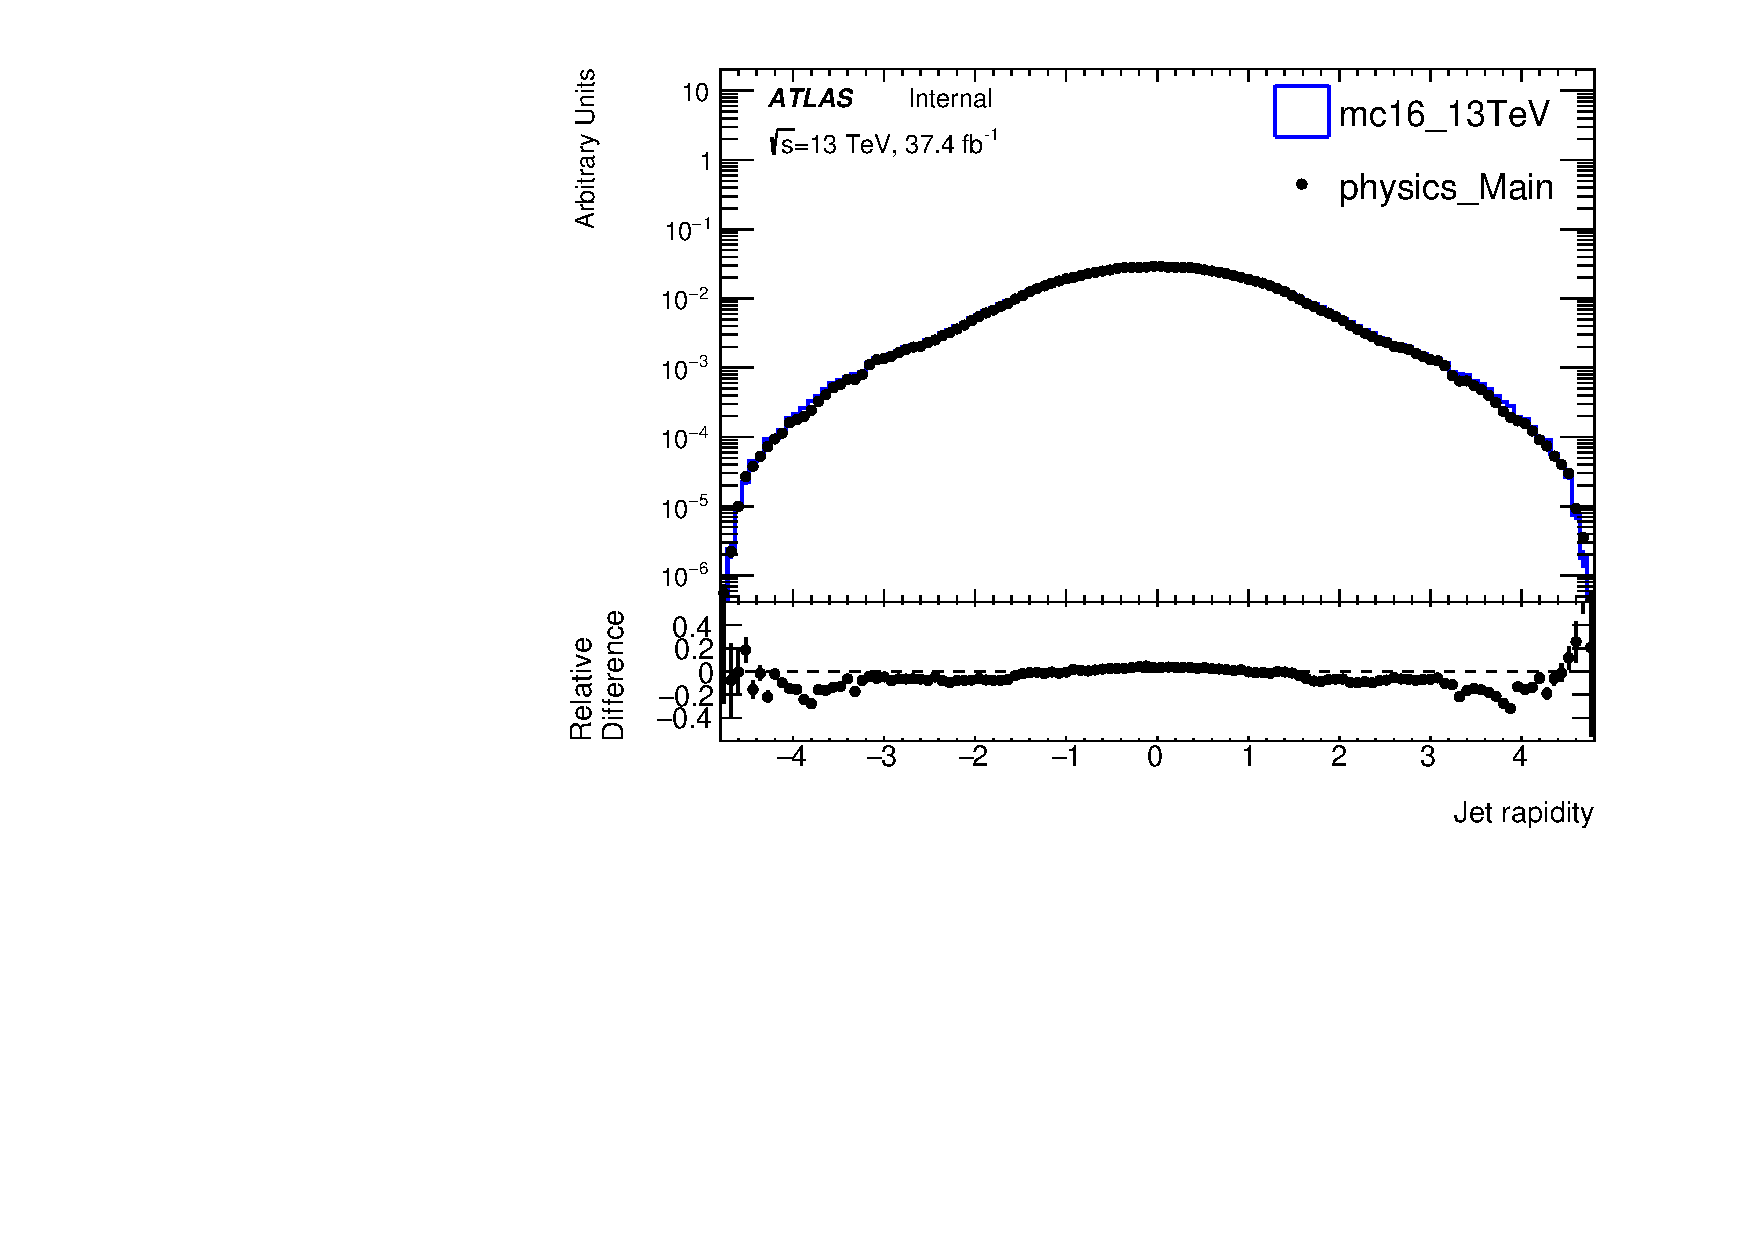
\includegraphics[width=0.45\textwidth]{figures/monitoring/resonant/2015-16/JJ/newStudy_jet_rapidity_logY_JJv01.pdf}}
 %
 
  \caption{Jet plots on %2016 data, 
  the resonant selection. (a) number of jets (b) $\Delta\phi$ between the two jets (c) jet $\eta$
  (d) jet $\phi$ (e) jet \pt\ (f) jet rapidity.  Fluctuations in the jet $phi$ distribution are attributable to dead modules in the tile calorimeter which lead to fewer jets in small slices of the detector.}
 \label{fig:JJmonitoring5}
\end{figure}


 \begin{figure}[htb]
 \centering
 %
 \subfigure[] {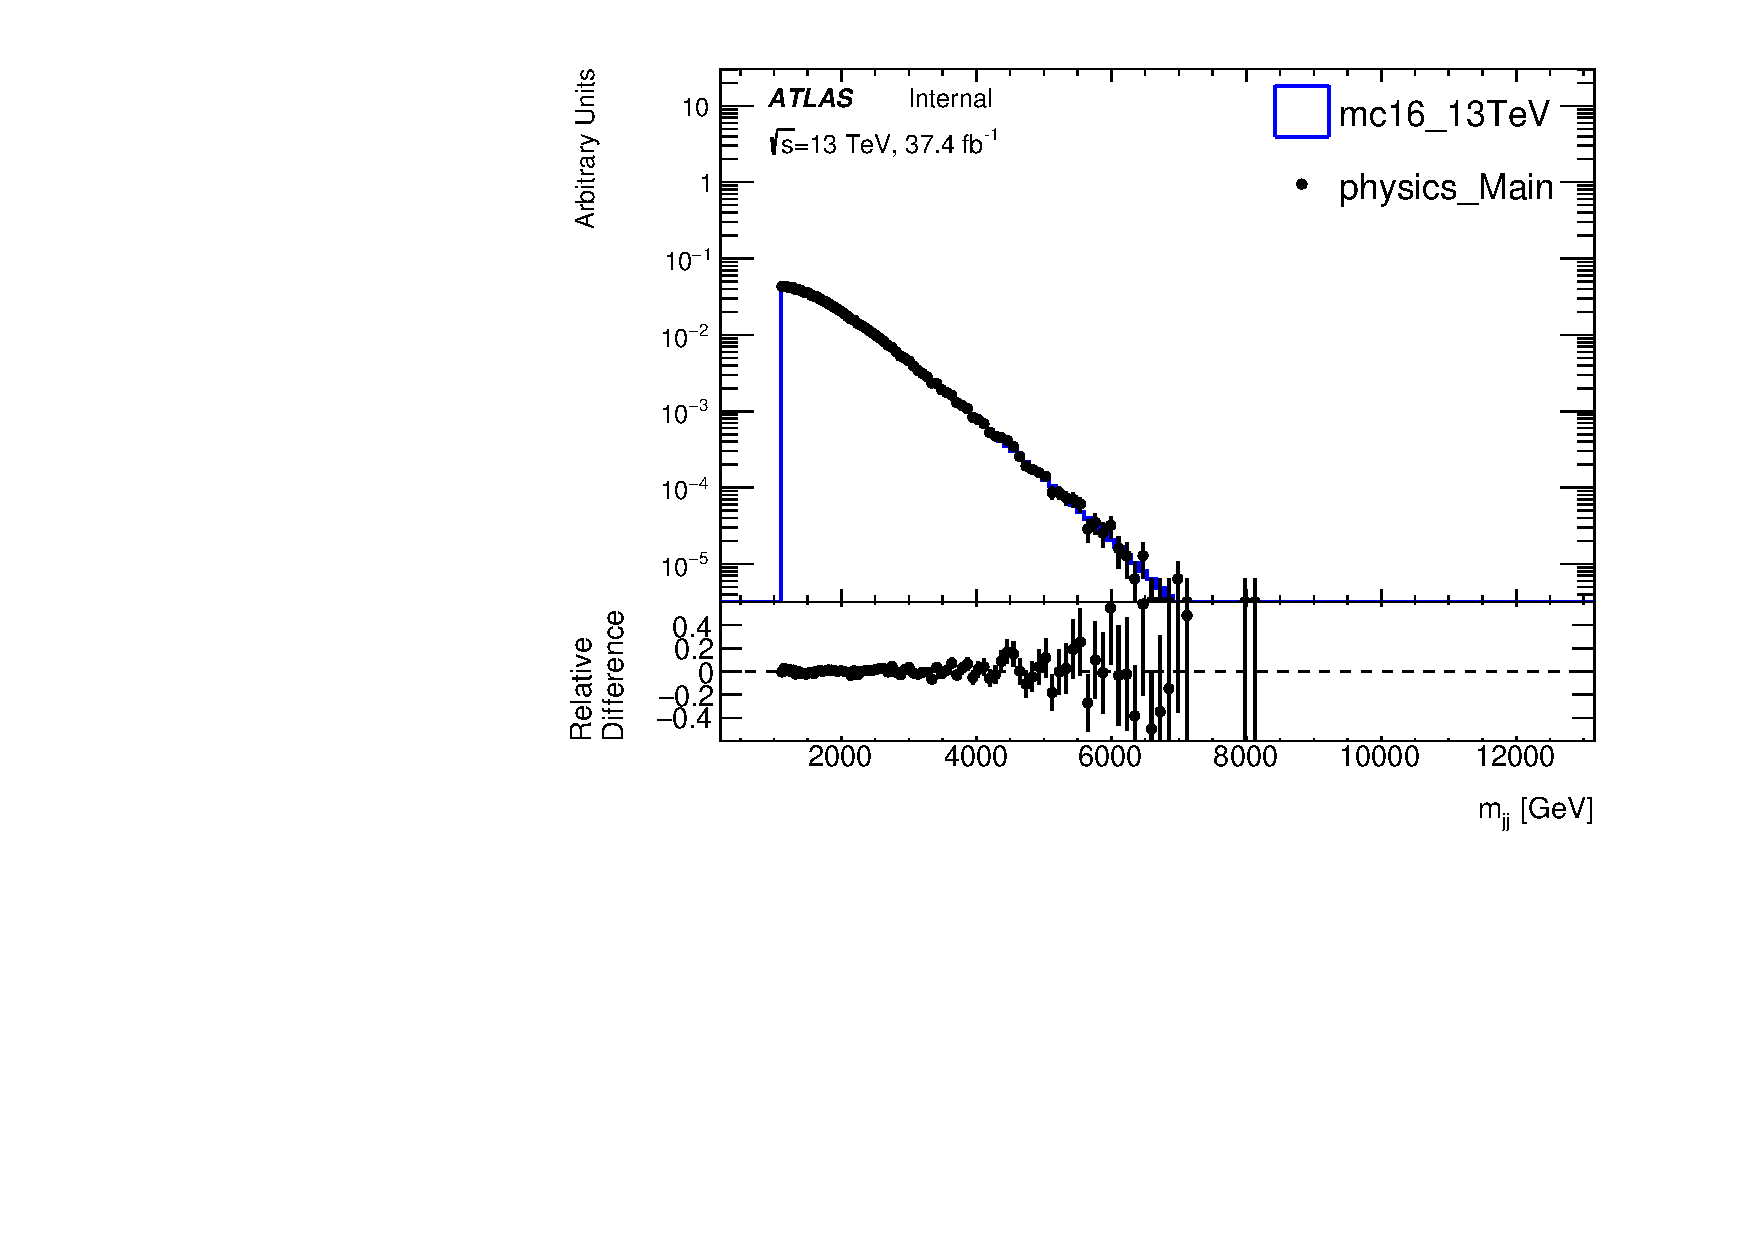
\includegraphics[width=0.45\textwidth]{figures/monitoring/resonant/2015-16/QQ/newStudy_mjj_logY_QQv01.pdf}}
 \subfigure[] {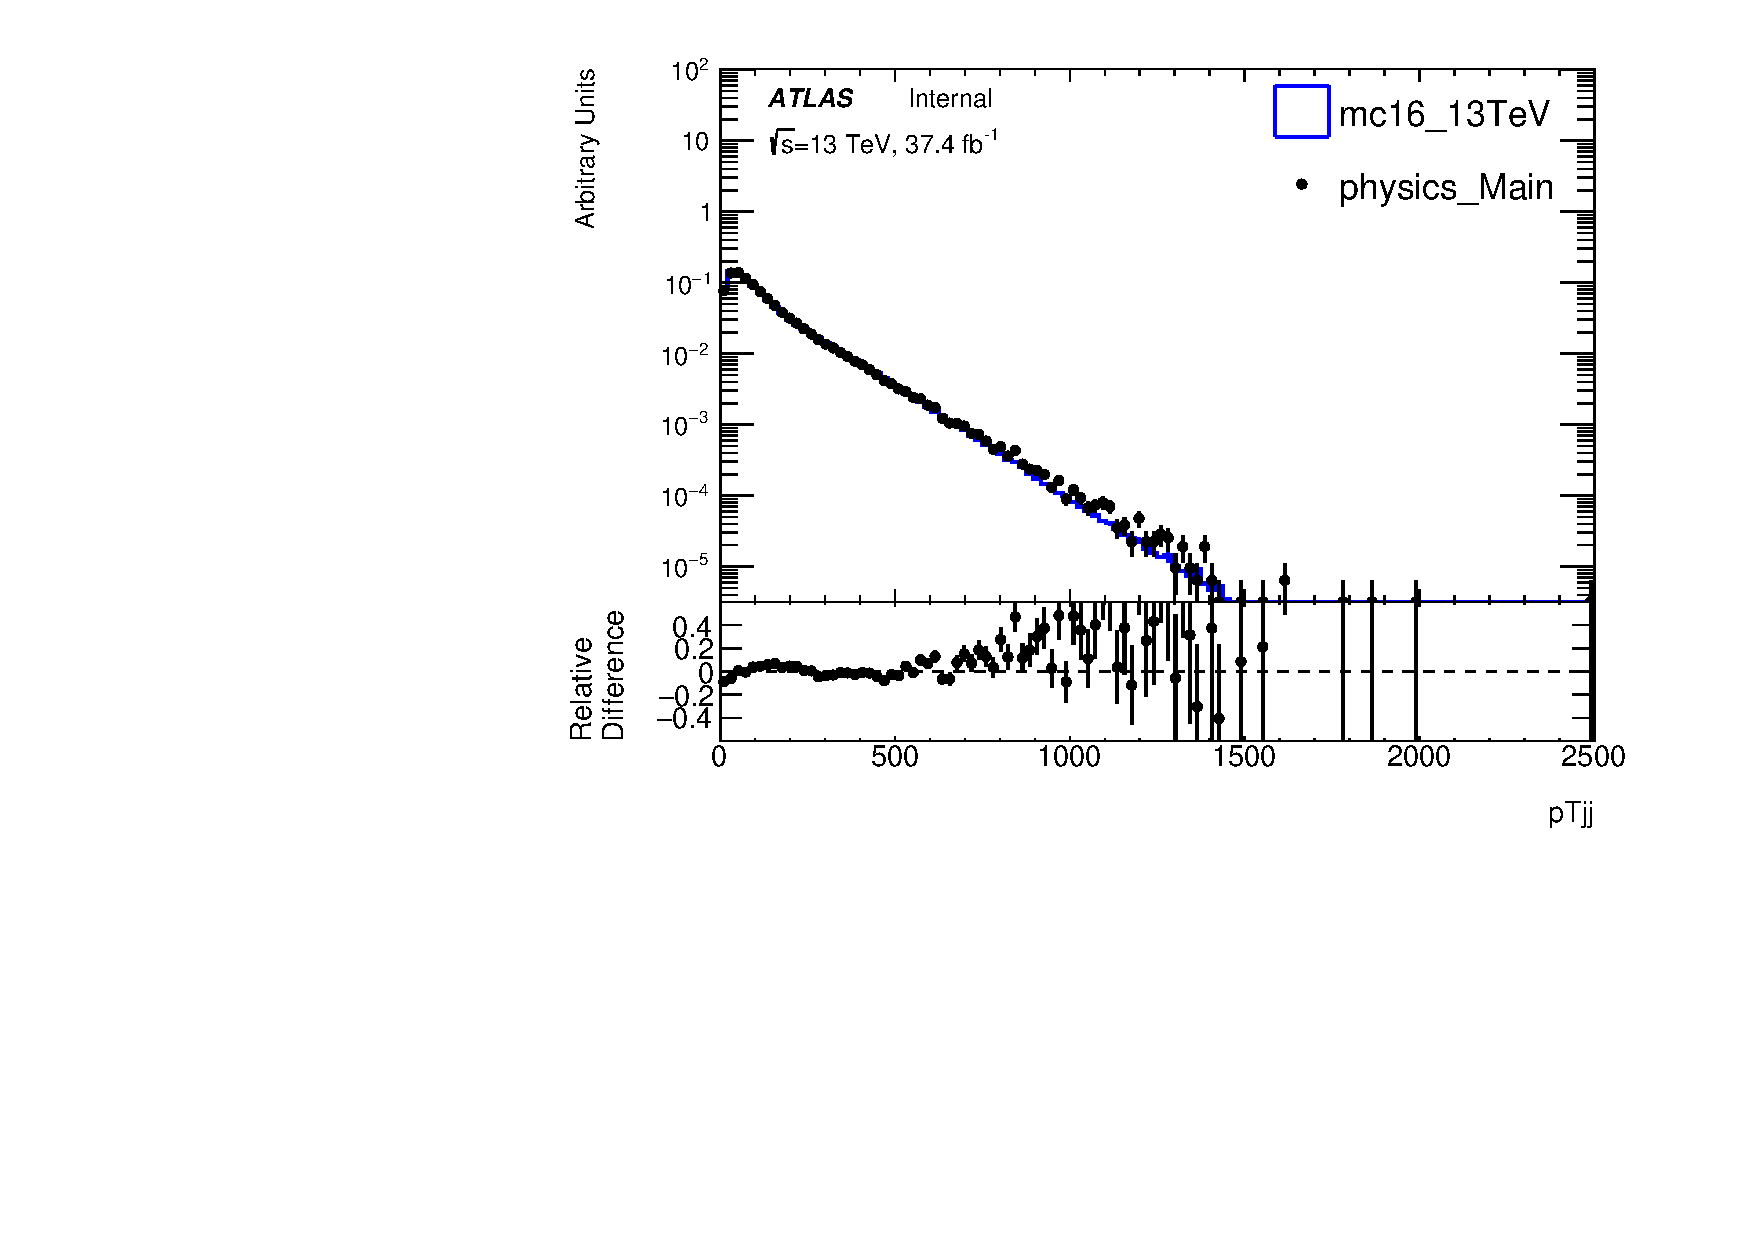
\includegraphics[width=0.45\textwidth]{figures/monitoring/resonant/2015-16/QQ/newStudy_pTjj_logY_QQv01.pdf}}
 %
 \subfigure[] {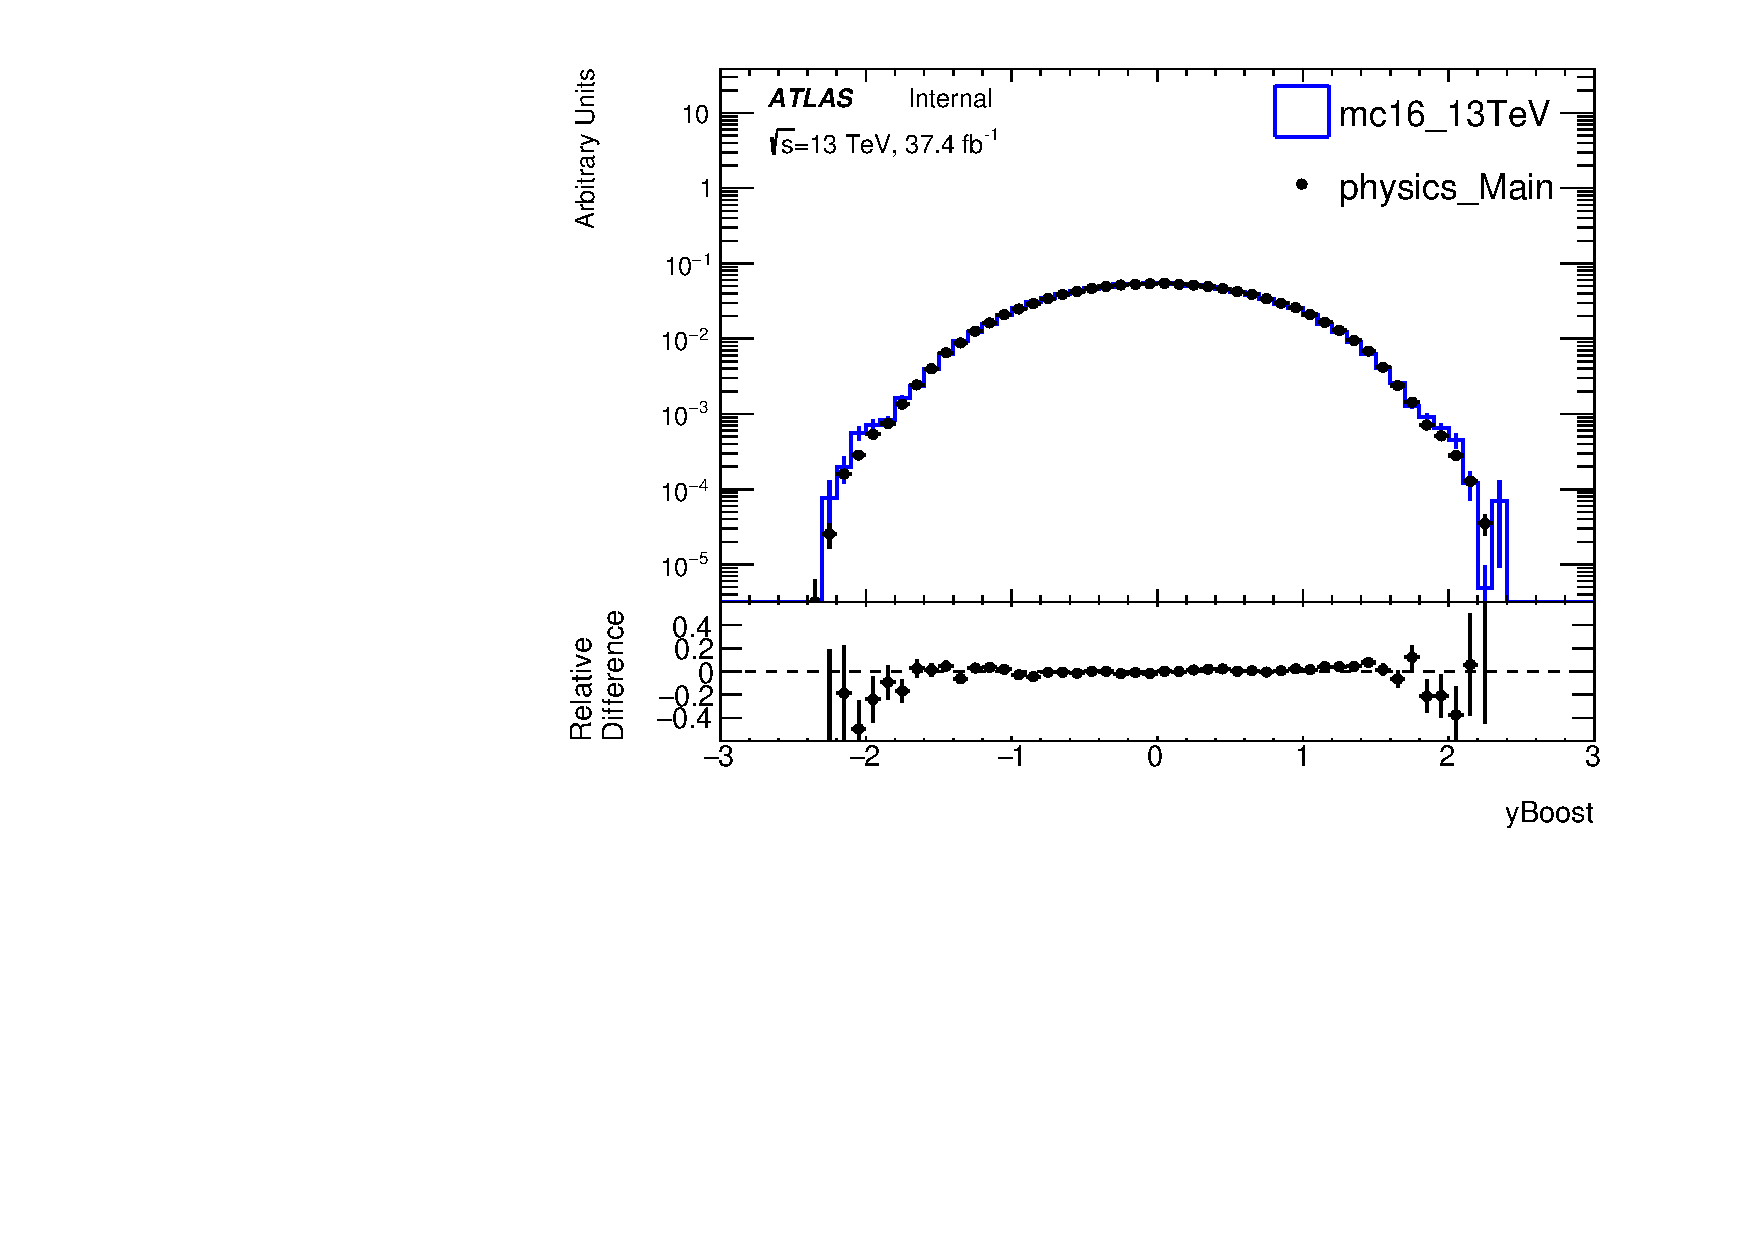
\includegraphics[width=0.45\textwidth]{figures/monitoring/resonant/2015-16/QQ/newStudy_yBoost_logY_QQv01.pdf}}
 \subfigure[] {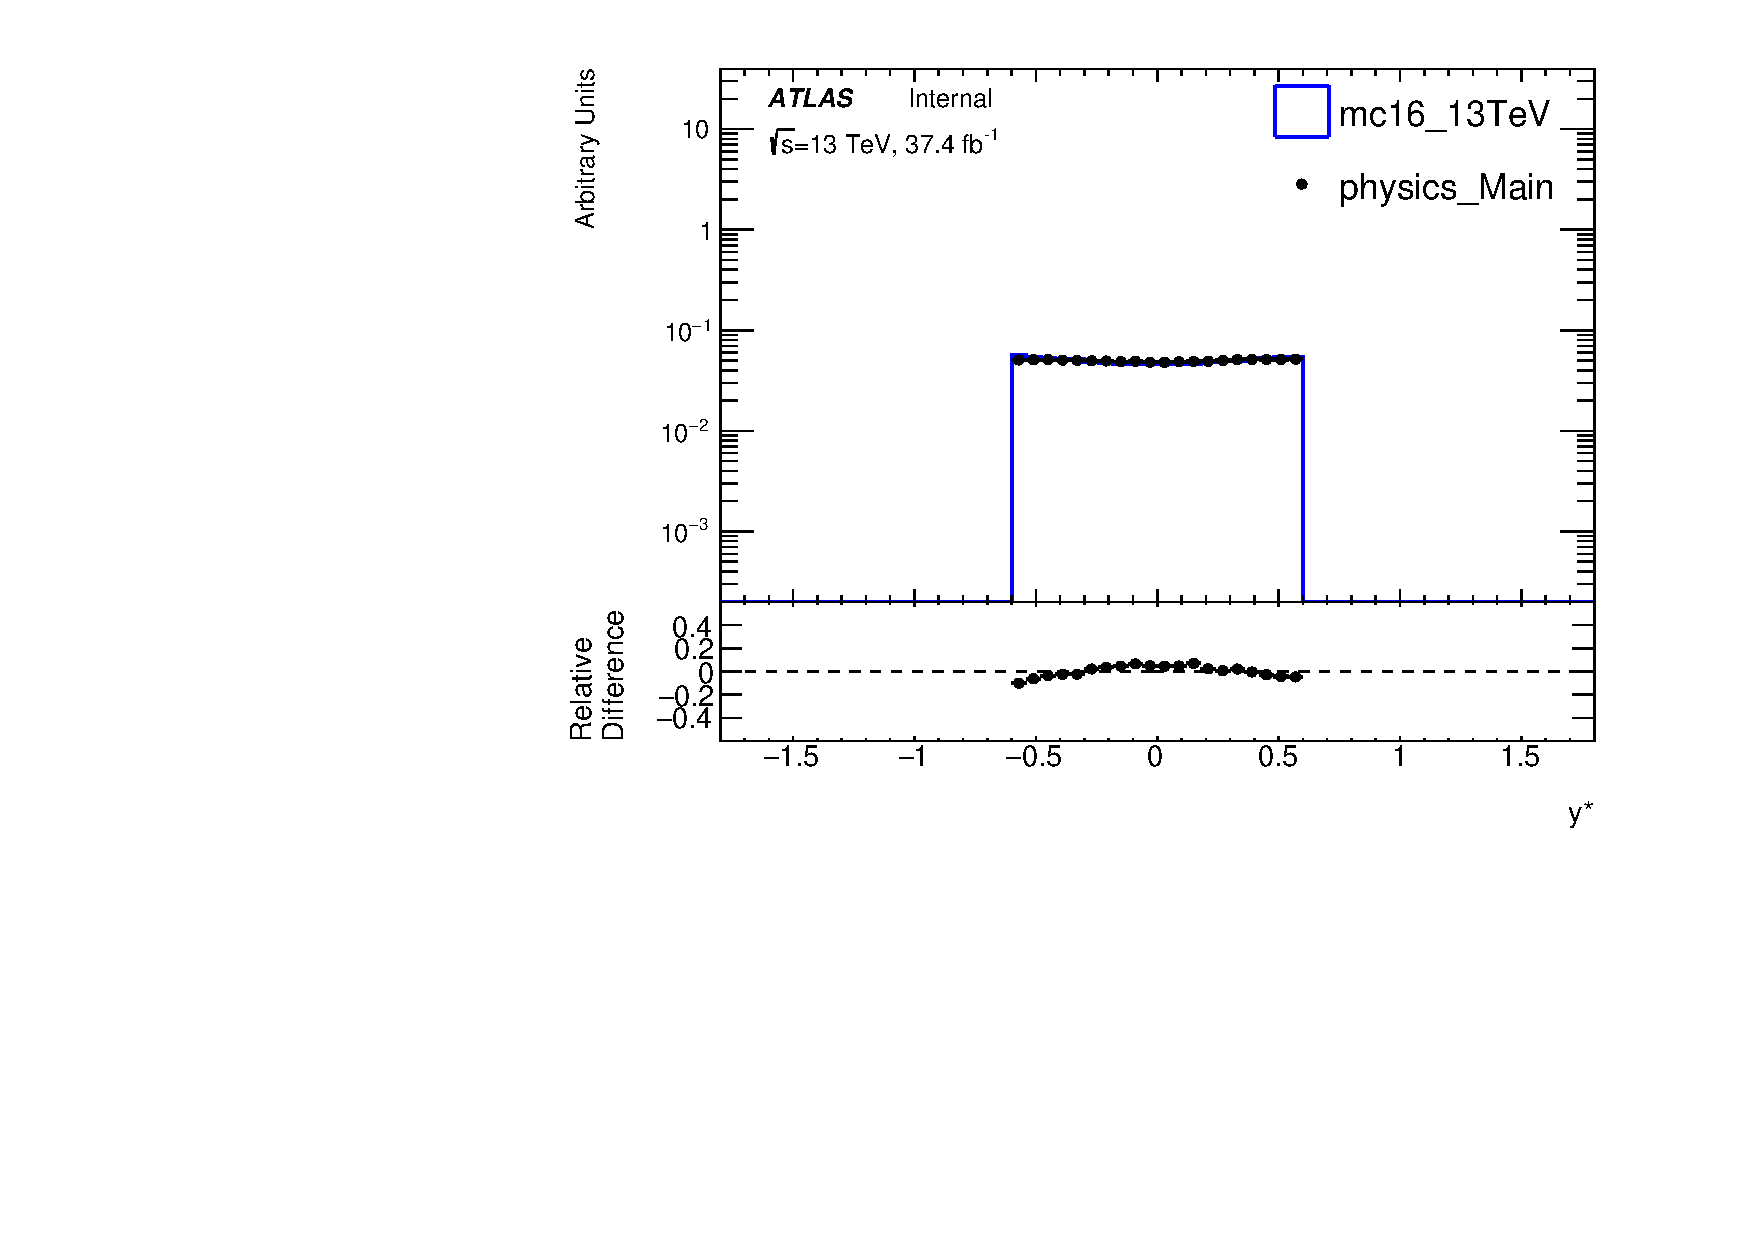
\includegraphics[width=0.45\textwidth]{figures/monitoring/resonant/2015-16/QQ/newStudy_yStar_logY_QQv01.pdf}}
 \caption{Jet plots on %2016 data, 
 the resonant selection. (a) dijet invariant mass (b) dijet \pt\ (c) \yB{} (d) \ystar{}. }
 \label{fig:JJmonitoring6}
\end{figure}


\clearpage


In this section a selection of kinematic and monitoring plots produced with the resonant selection on the QQ dataset is shown 
(Figures~\ref{fig:QQmonitoring1},  
\ref{fig:QQmonitoring5}, \ref{fig:QQmonitoring6}). These plots are relative to \integLumi of data collected in 2015 and 2016.
 GRL has been applied here.

\begin{figure}[htb]
 \centering
 \subfigure[] {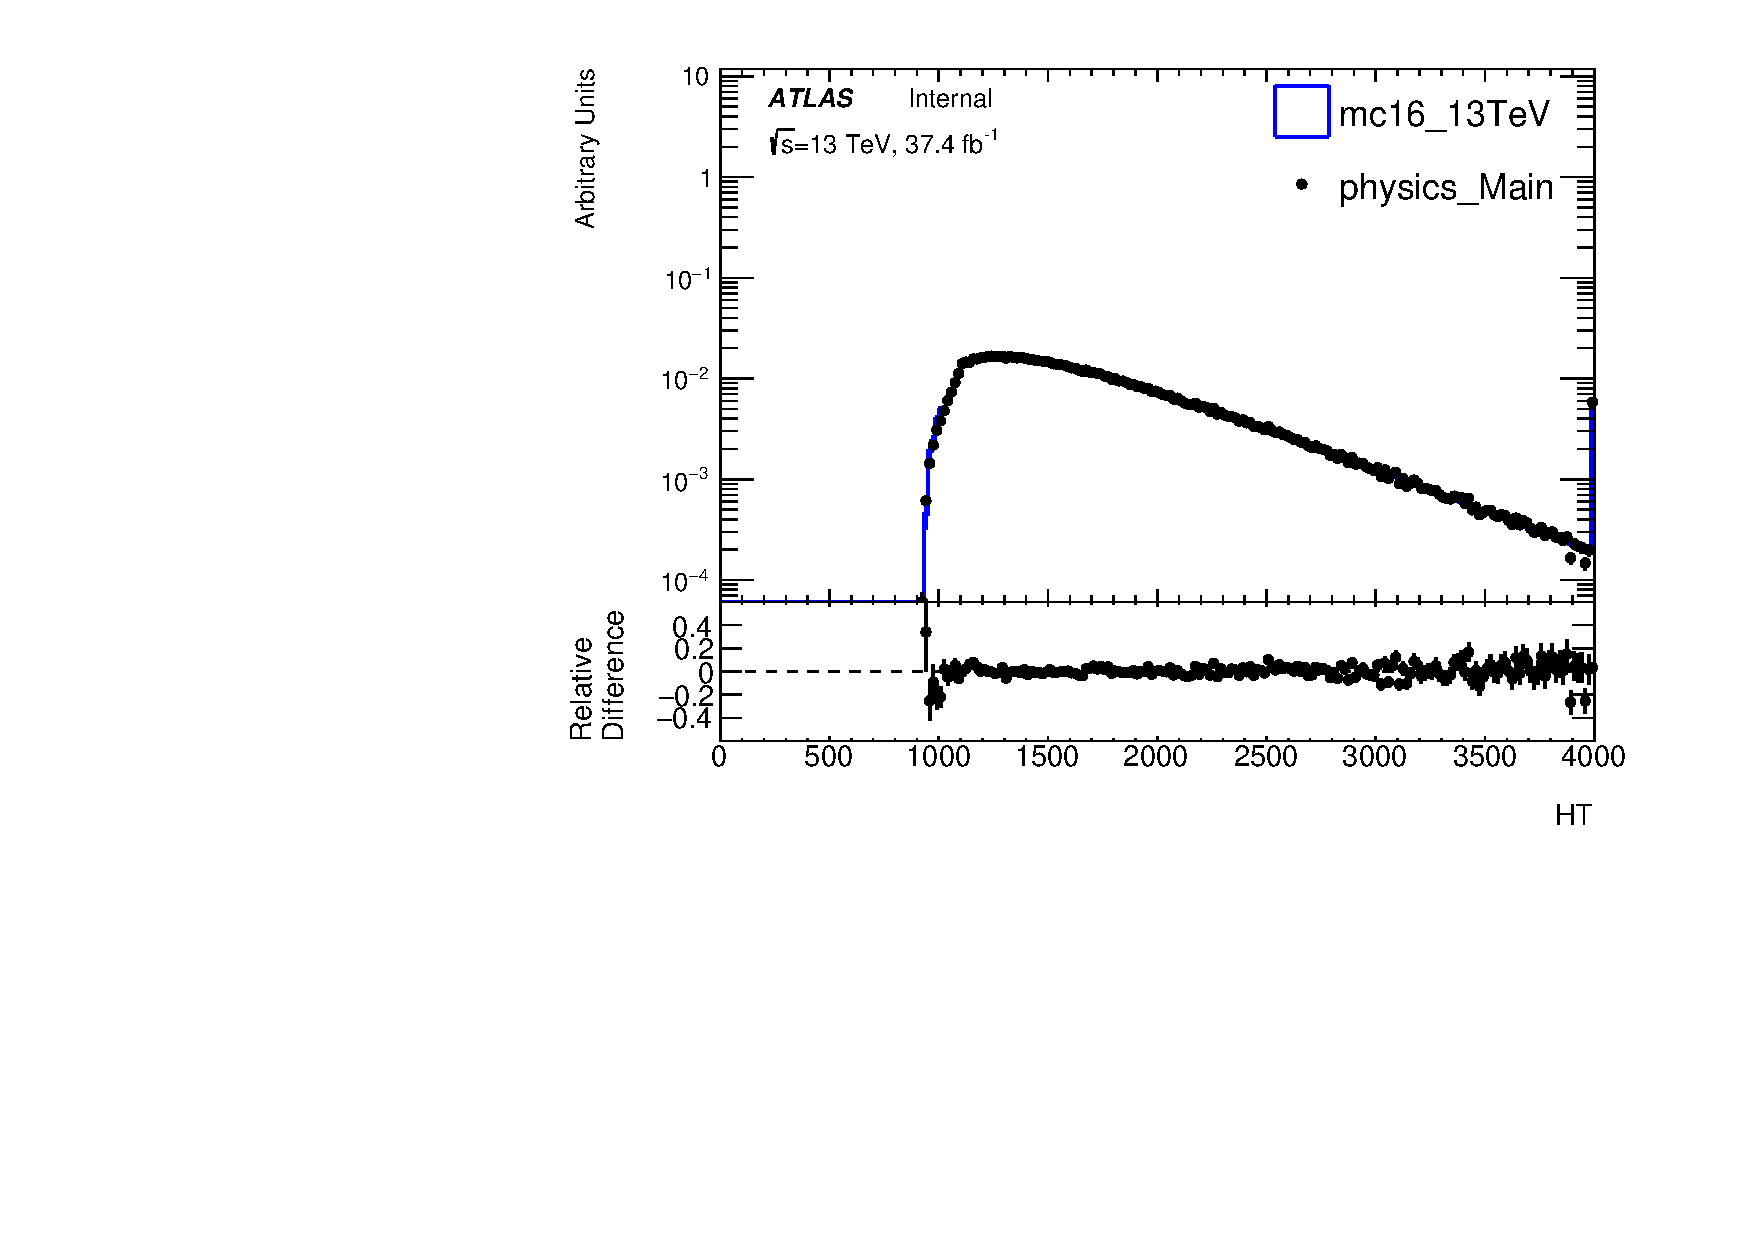
\includegraphics[width=0.45\textwidth]{figures/monitoring/resonant/2015-16/QQ/newStudy_HT_logY_QQv01.pdf}}
 \subfigure[] {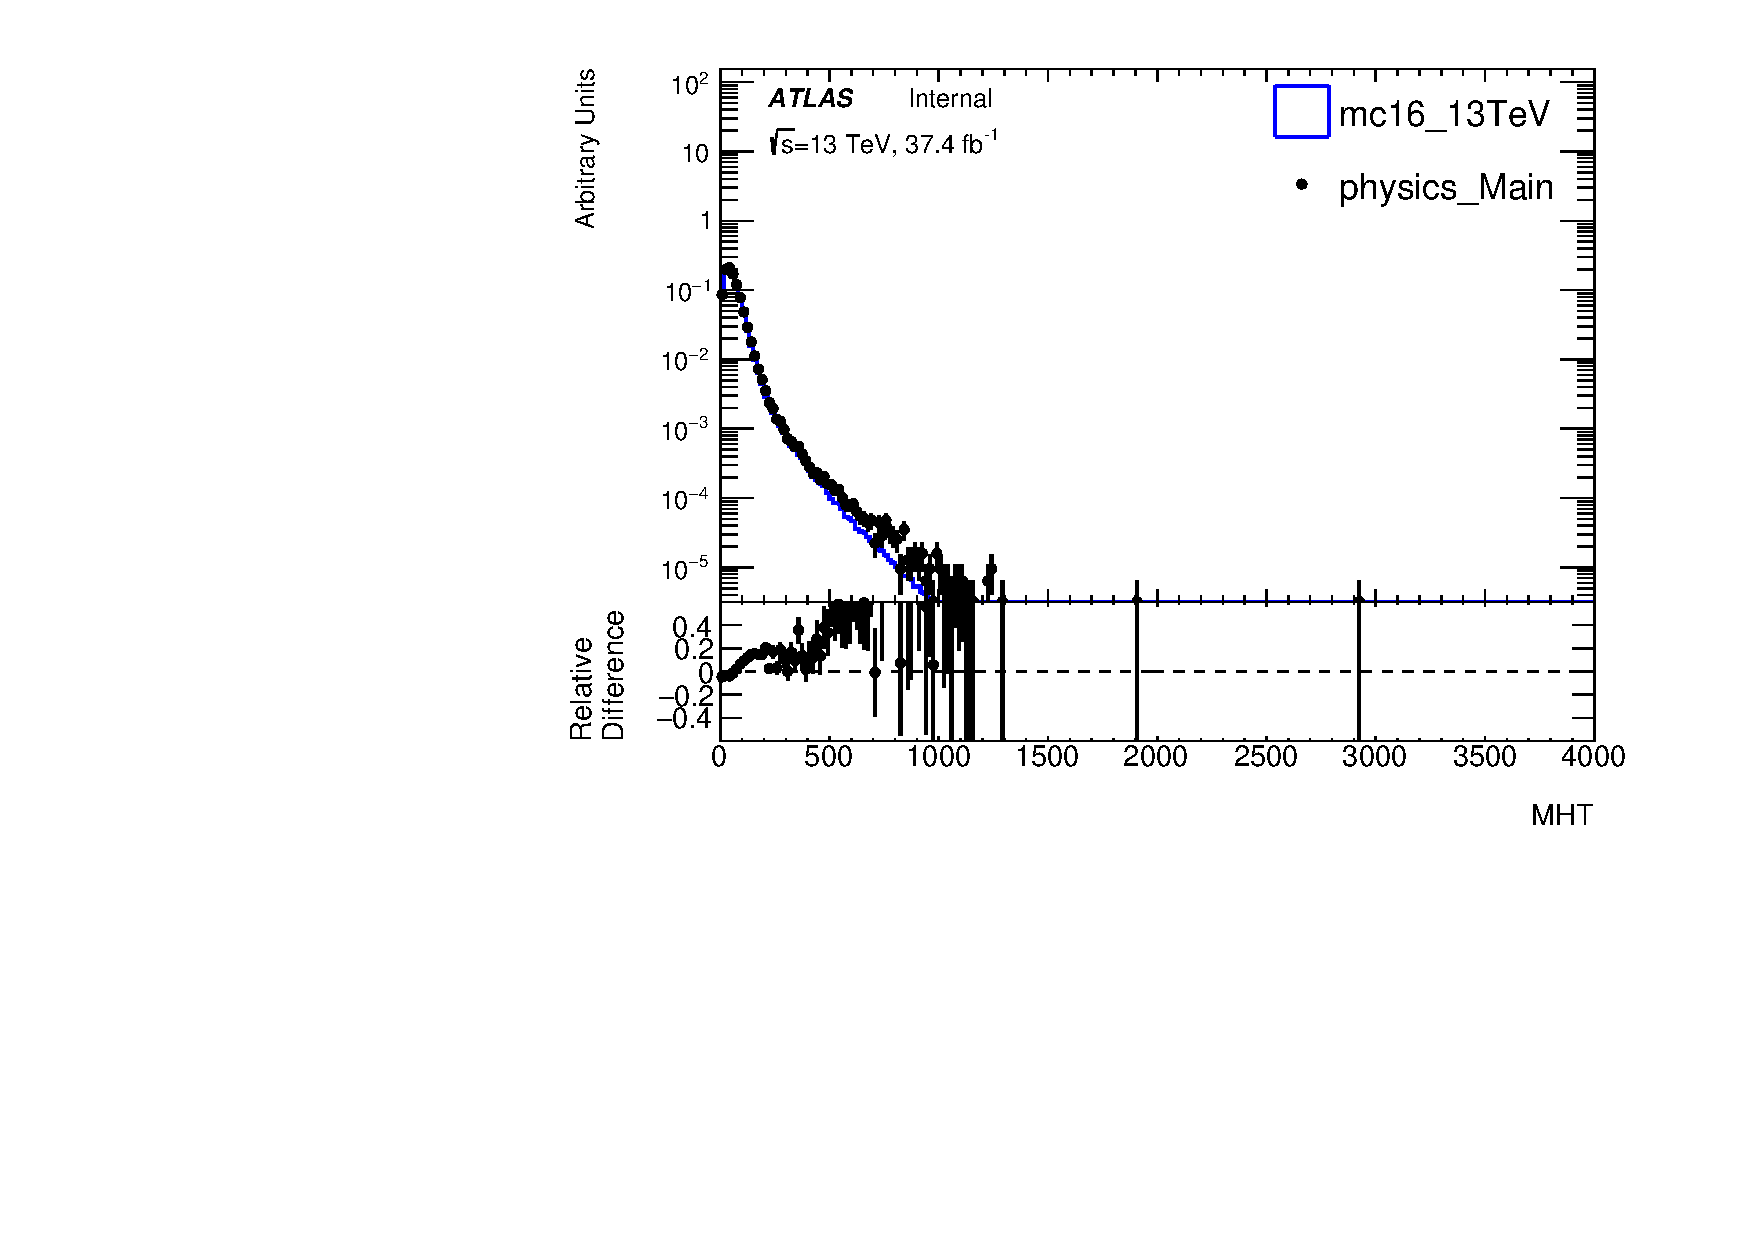
\includegraphics[width=0.45\textwidth]{figures/monitoring/resonant/2015-16/QQ/newStudy_MHT_logY_QQv01.pdf}}
 %
 \subfigure[] {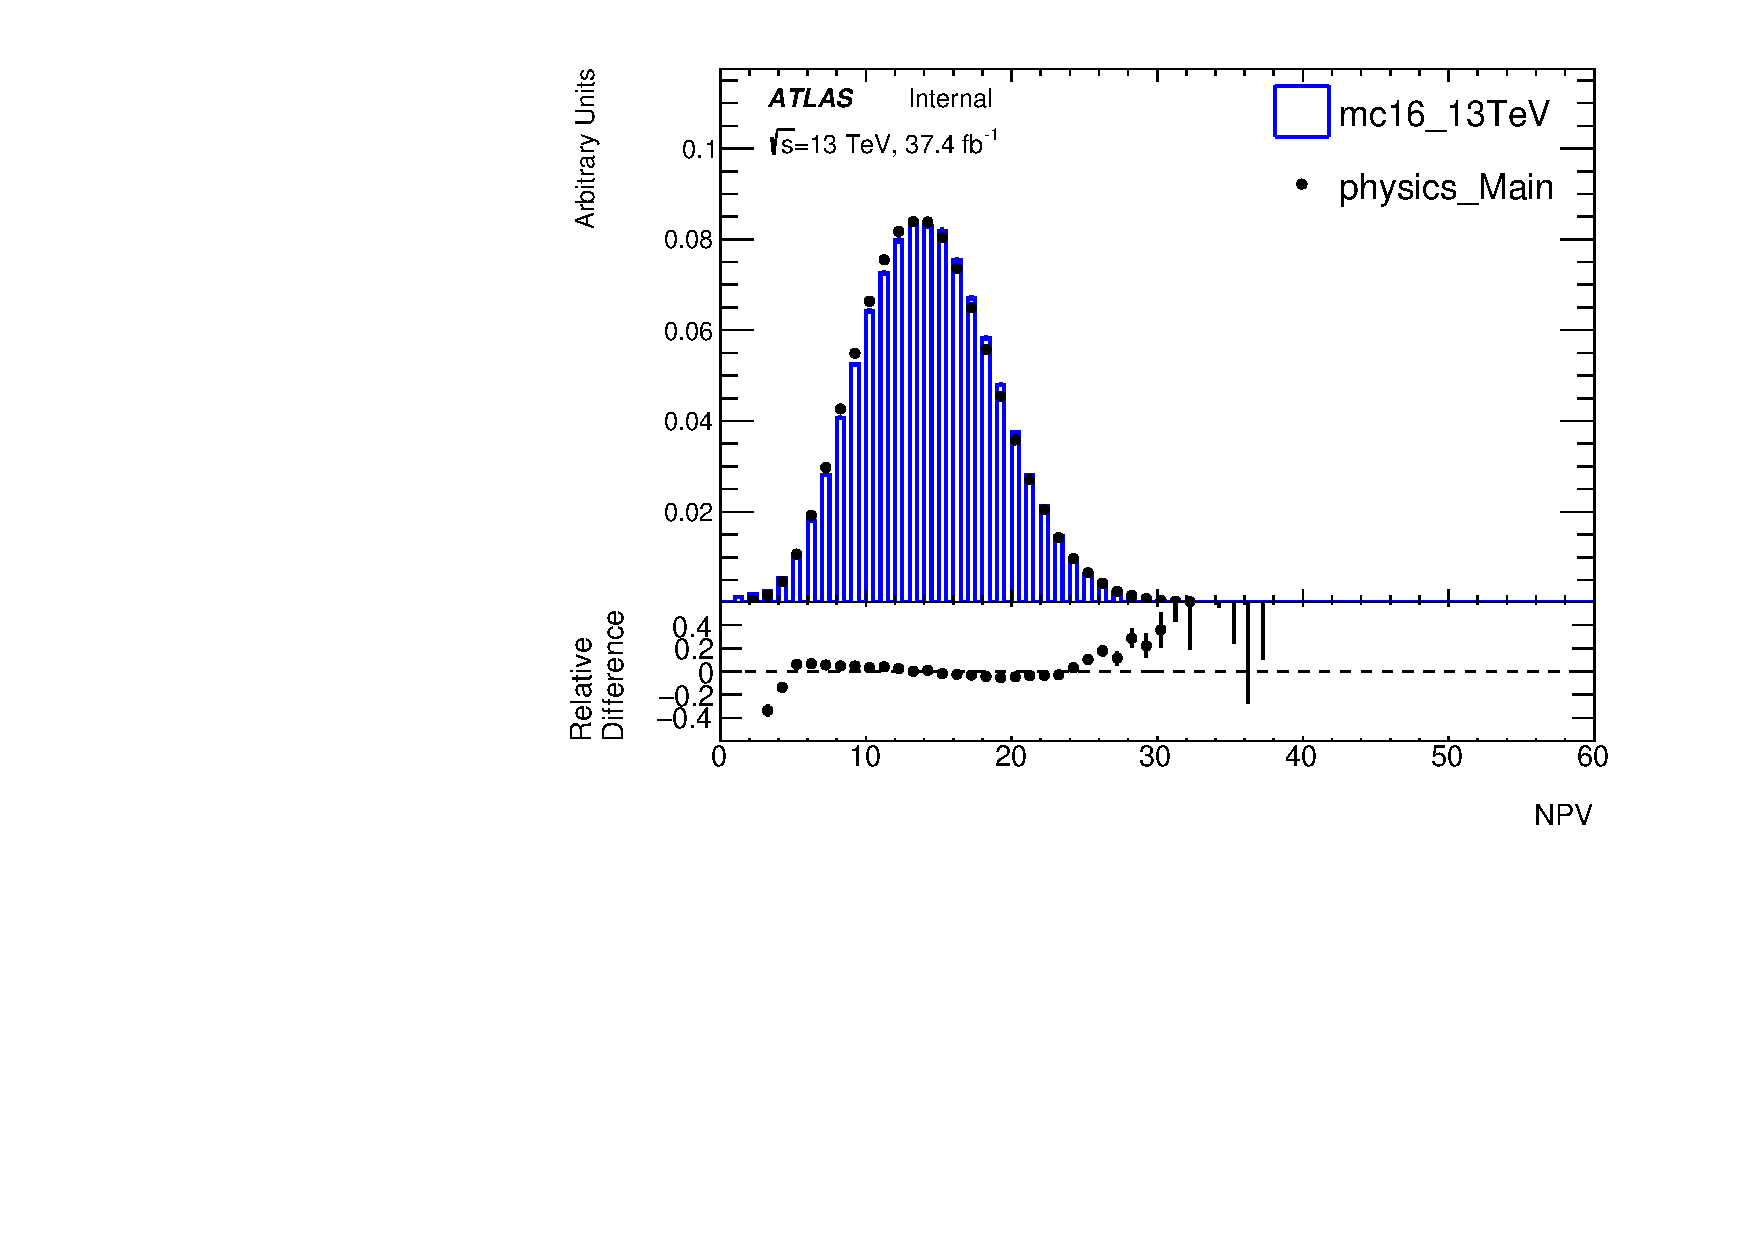
\includegraphics[width=0.45\textwidth]{figures/monitoring/resonant/2015-16/QQ/newStudy_NPV_QQv01.pdf}}
 \subfigure[] {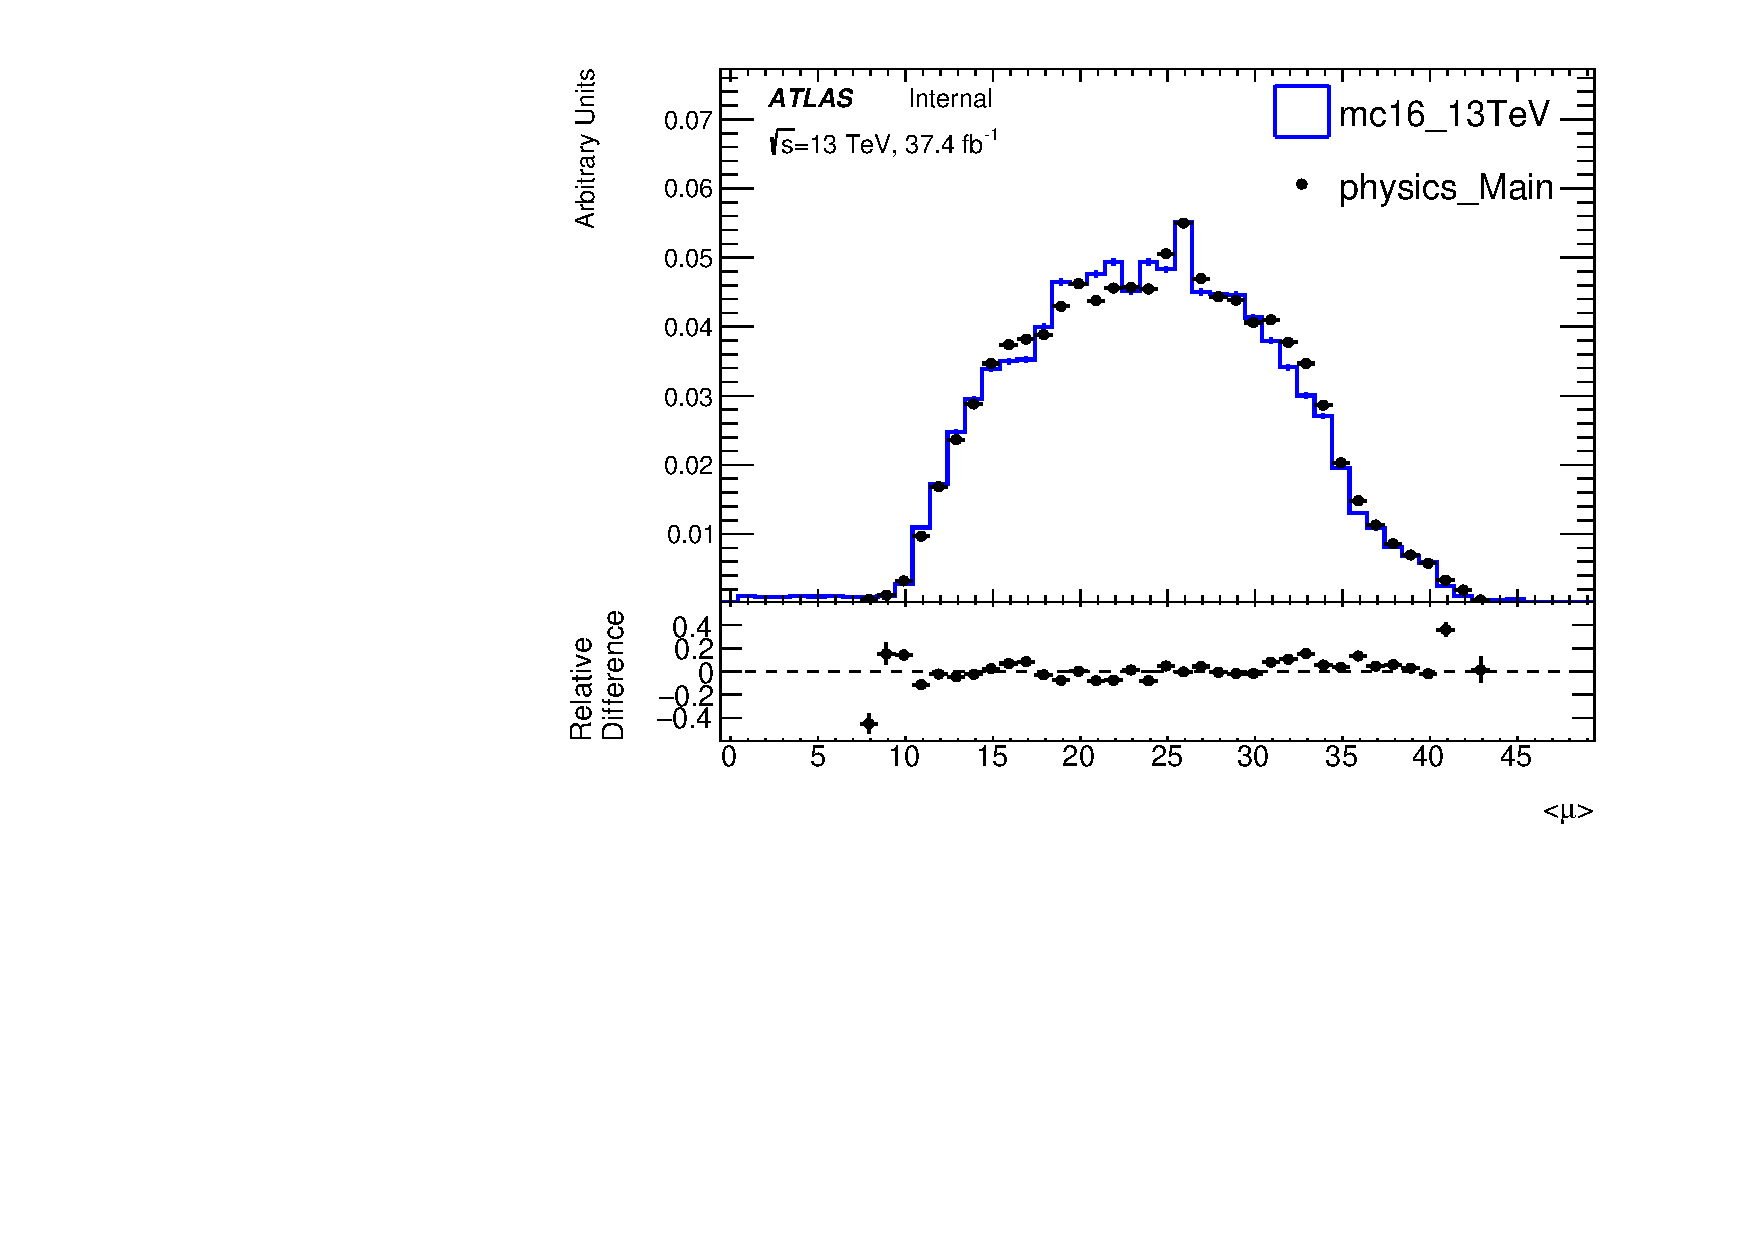
\includegraphics[width=0.45\textwidth]{figures/monitoring/resonant/2015-16/QQ/newStudy_averageInteractionsPerCrossing_QQv01.pdf}}
 %

 \caption{Monitoring plots on %2016 data, 
 the QQ resonant selection. (a) $H_T$, (b) $MH_T$ (missing transverse momentum calculated only from the jets in the event), (c) number of primary interaction vertices and (d) average interactions per bunch crossing.}
 \label{fig:QQmonitoring1}
\end{figure}

 \begin{figure}[htb]
 \centering
  %
 \subfigure[] {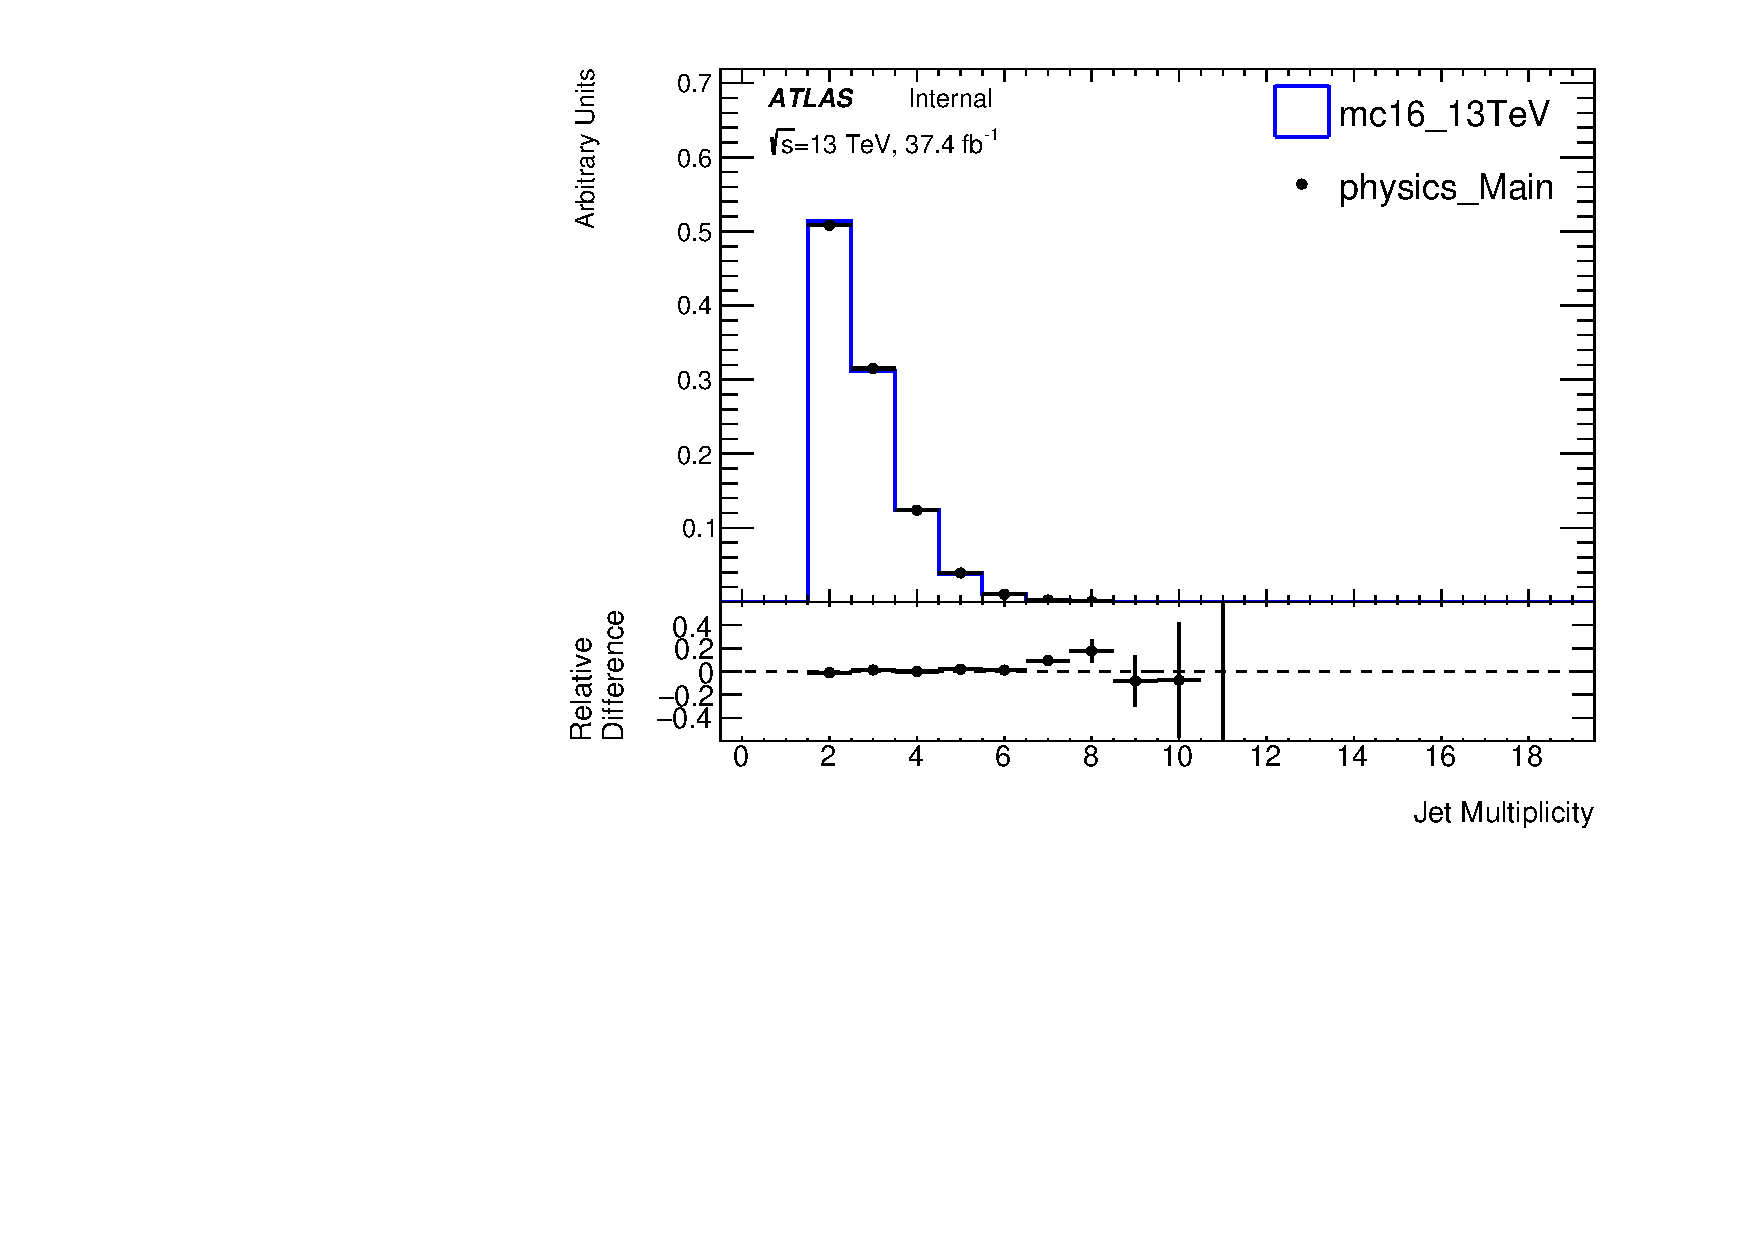
\includegraphics[width=0.45\textwidth]{figures/monitoring/resonant/2015-16/QQ/newStudy_njets_QQv01.pdf}}
 \subfigure[] {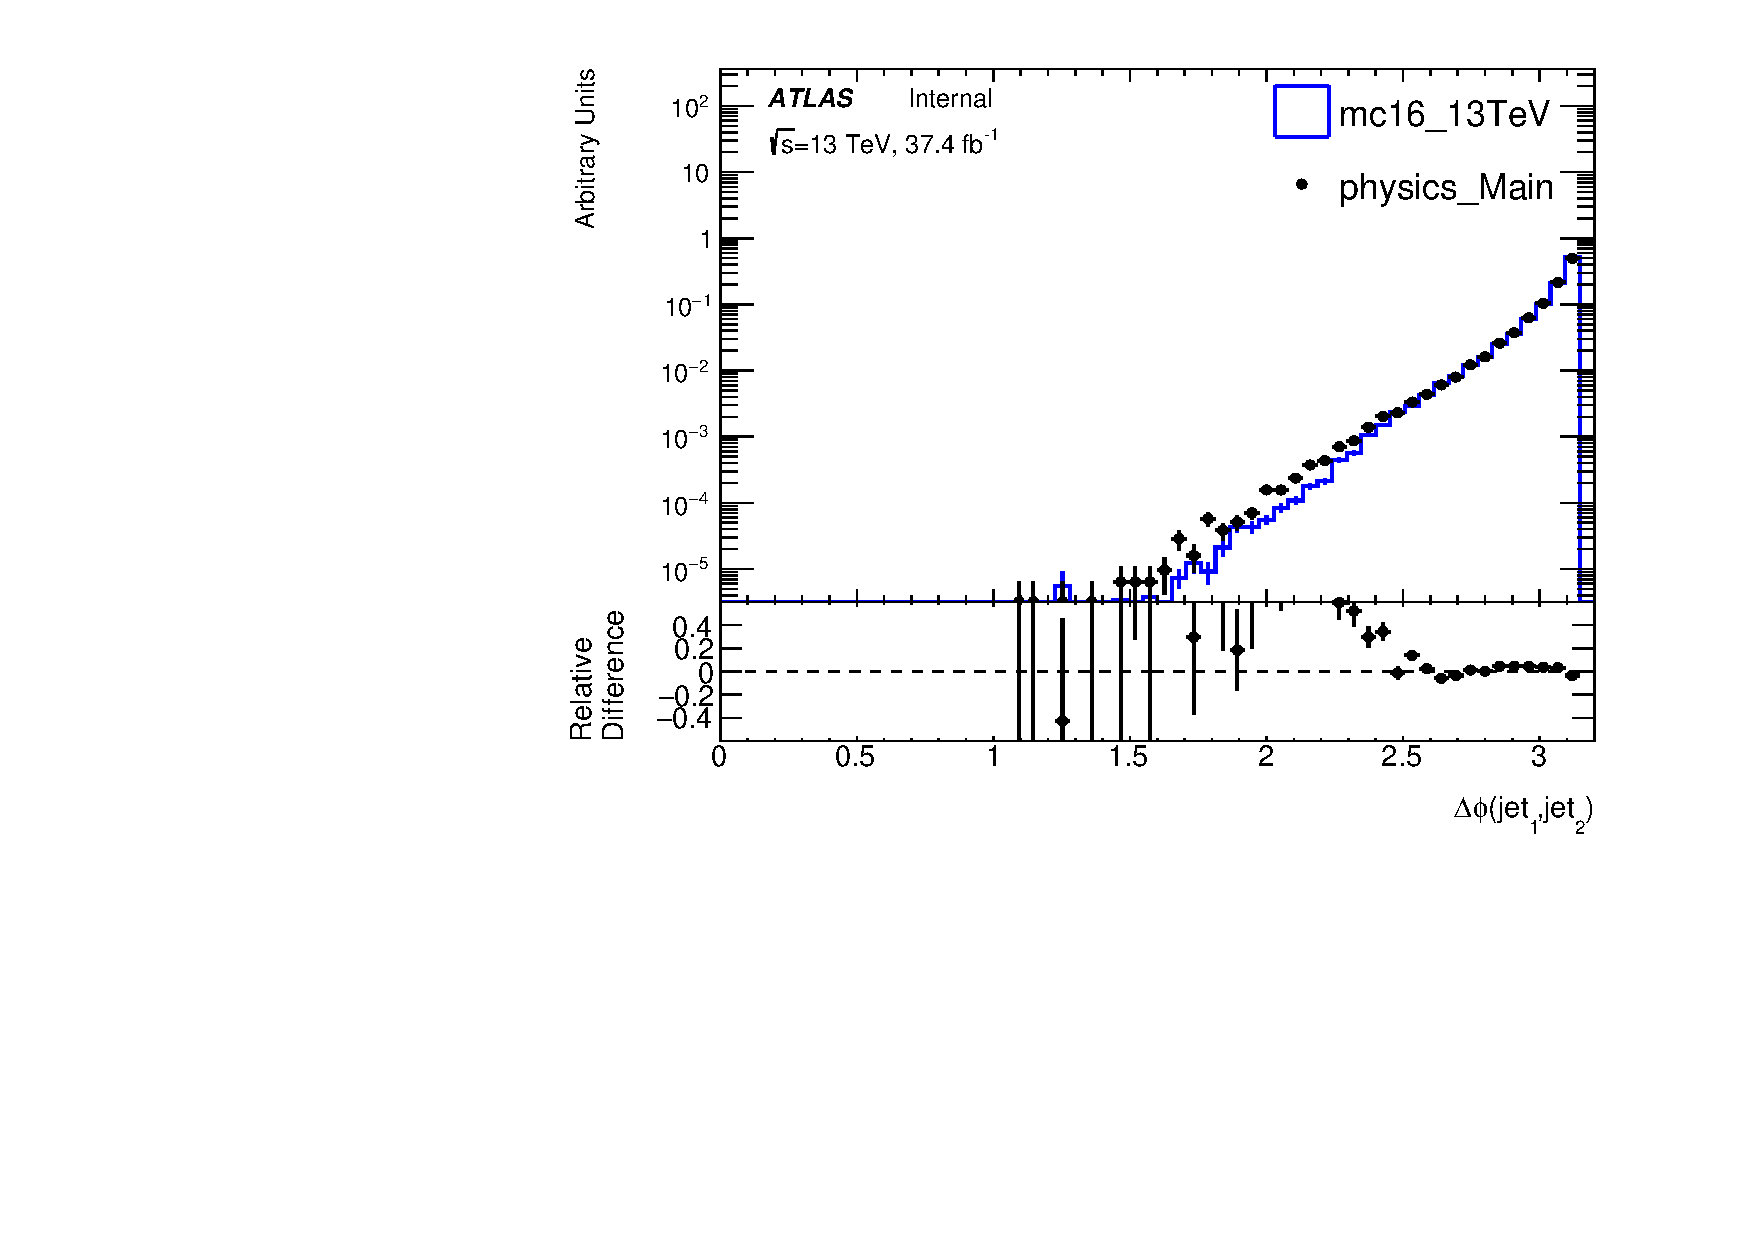
\includegraphics[width=0.45\textwidth]{figures/monitoring/resonant/2015-16/QQ//newStudy_deltaPhi_logY_QQv01.pdf}}

%
 \subfigure[] {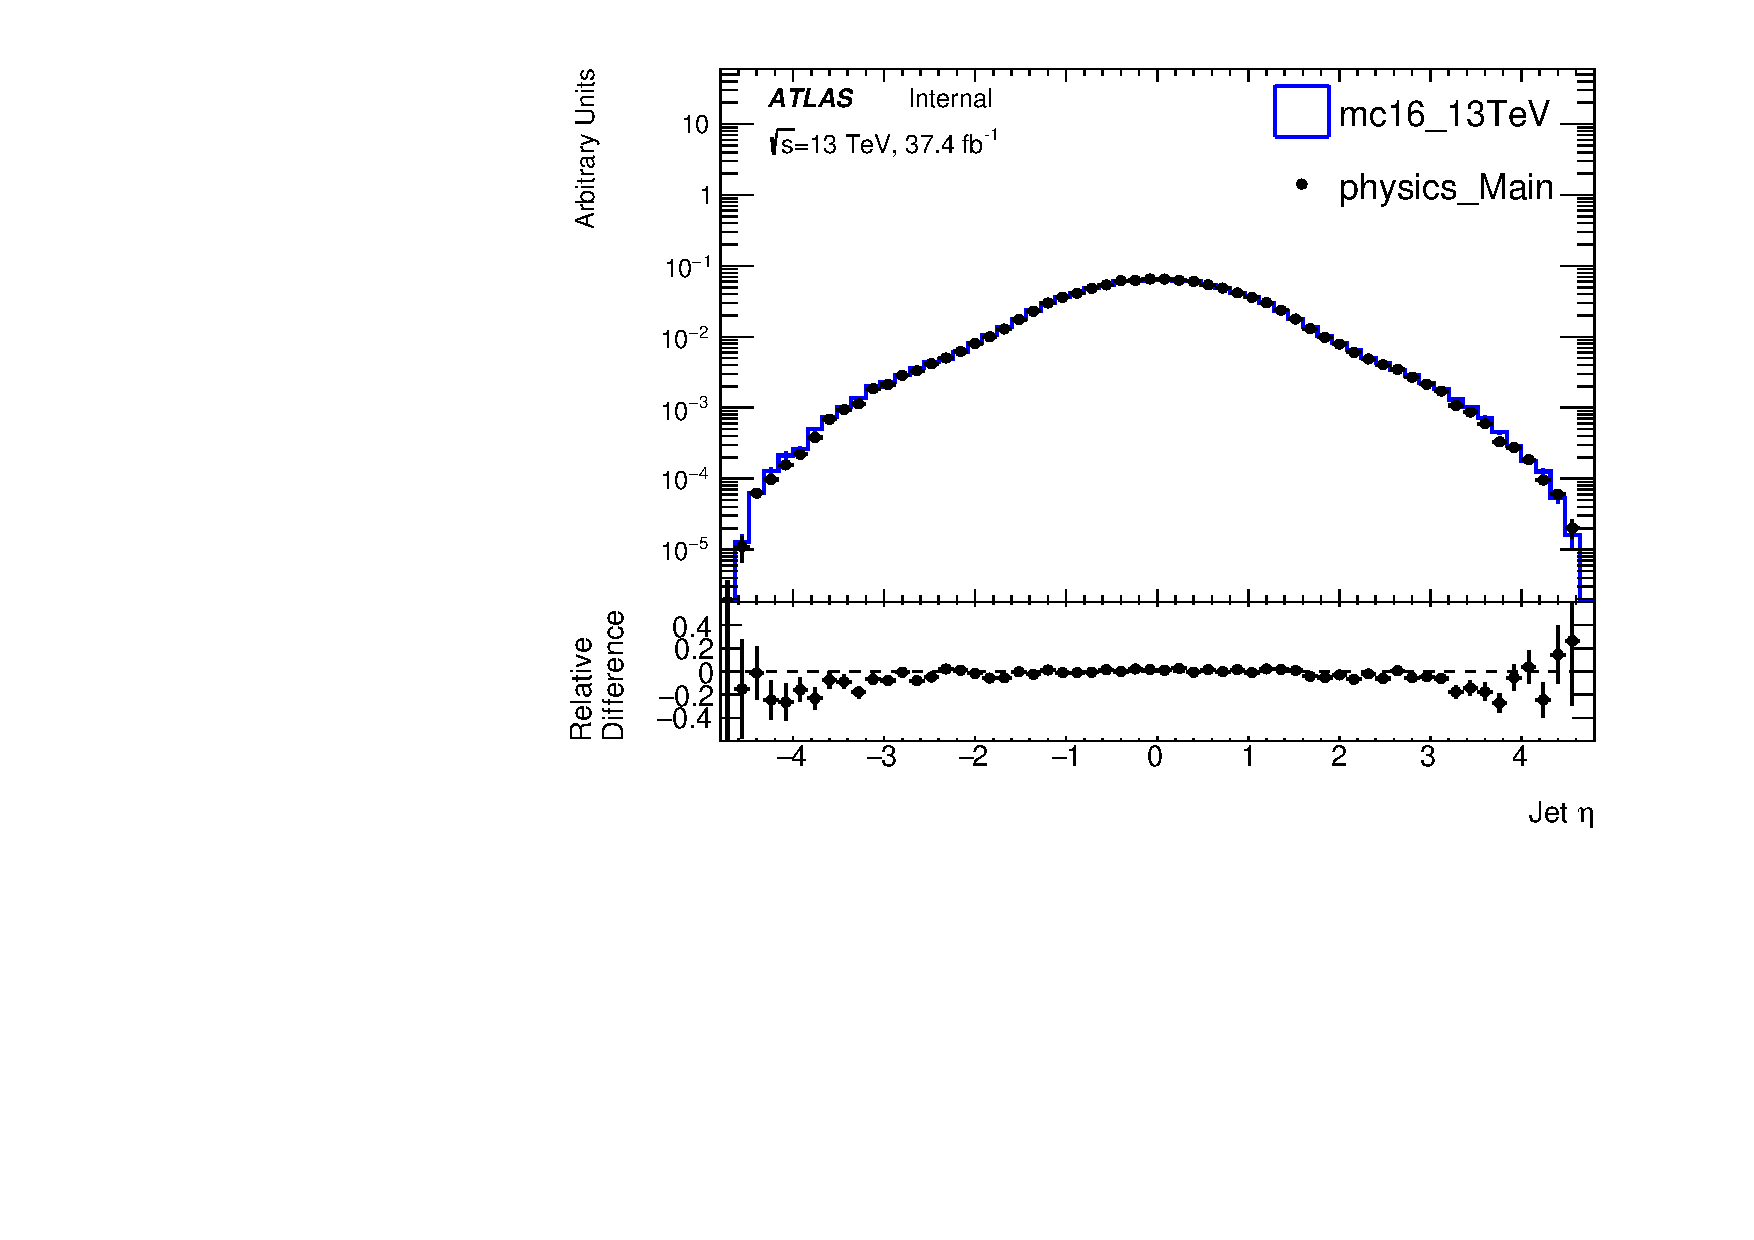
\includegraphics[width=0.45\textwidth]{figures/monitoring/resonant/2015-16/QQ/newStudy_jet_eta_logY_QQv01.pdf}}
 \subfigure[] {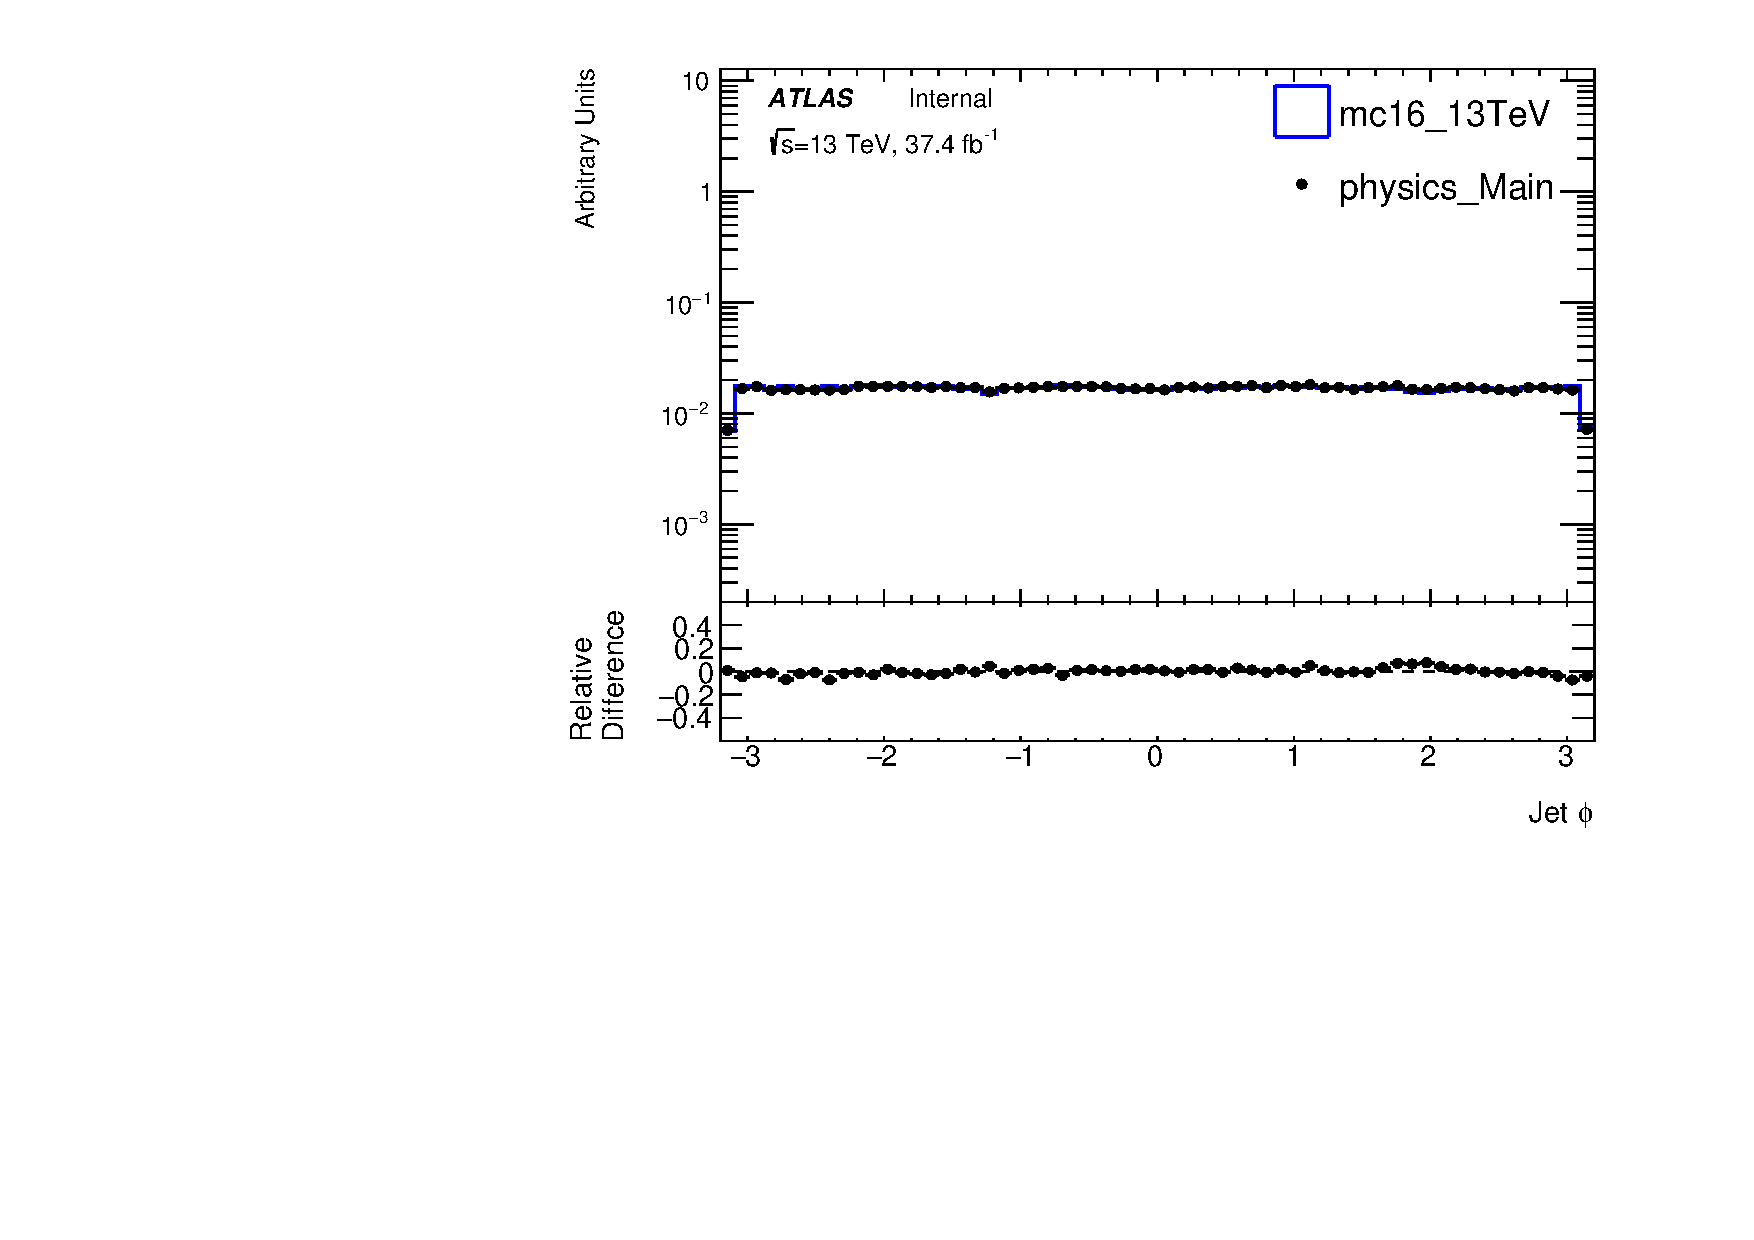
\includegraphics[width=0.45\textwidth]{figures/monitoring/resonant/2015-16/QQ/newStudy_jet_phi_logY_QQv01.pdf}}
 %
 \subfigure[] {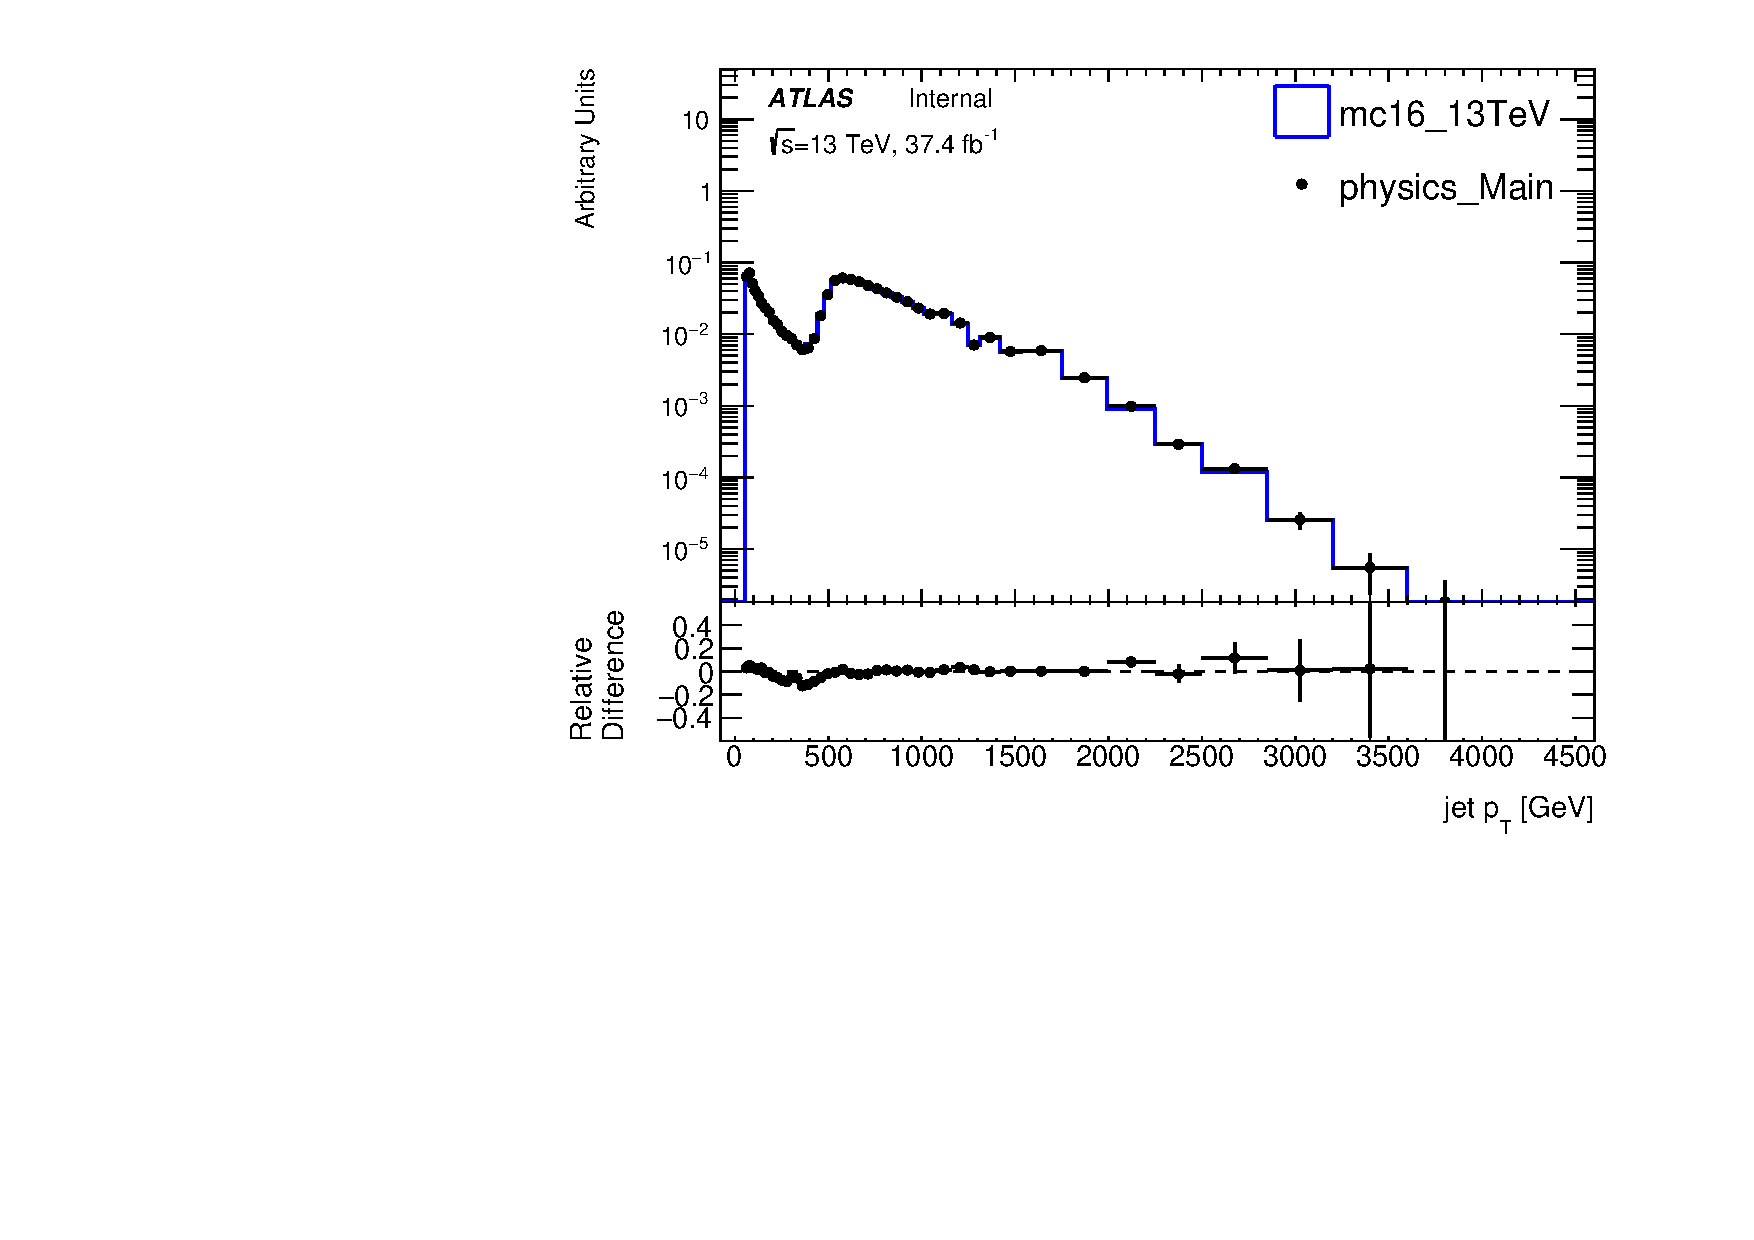
\includegraphics[width=0.45\textwidth]{figures/monitoring/resonant/2015-16/QQ/newStudy_jet_pt_logY_QQv01.pdf}}
 \subfigure[] {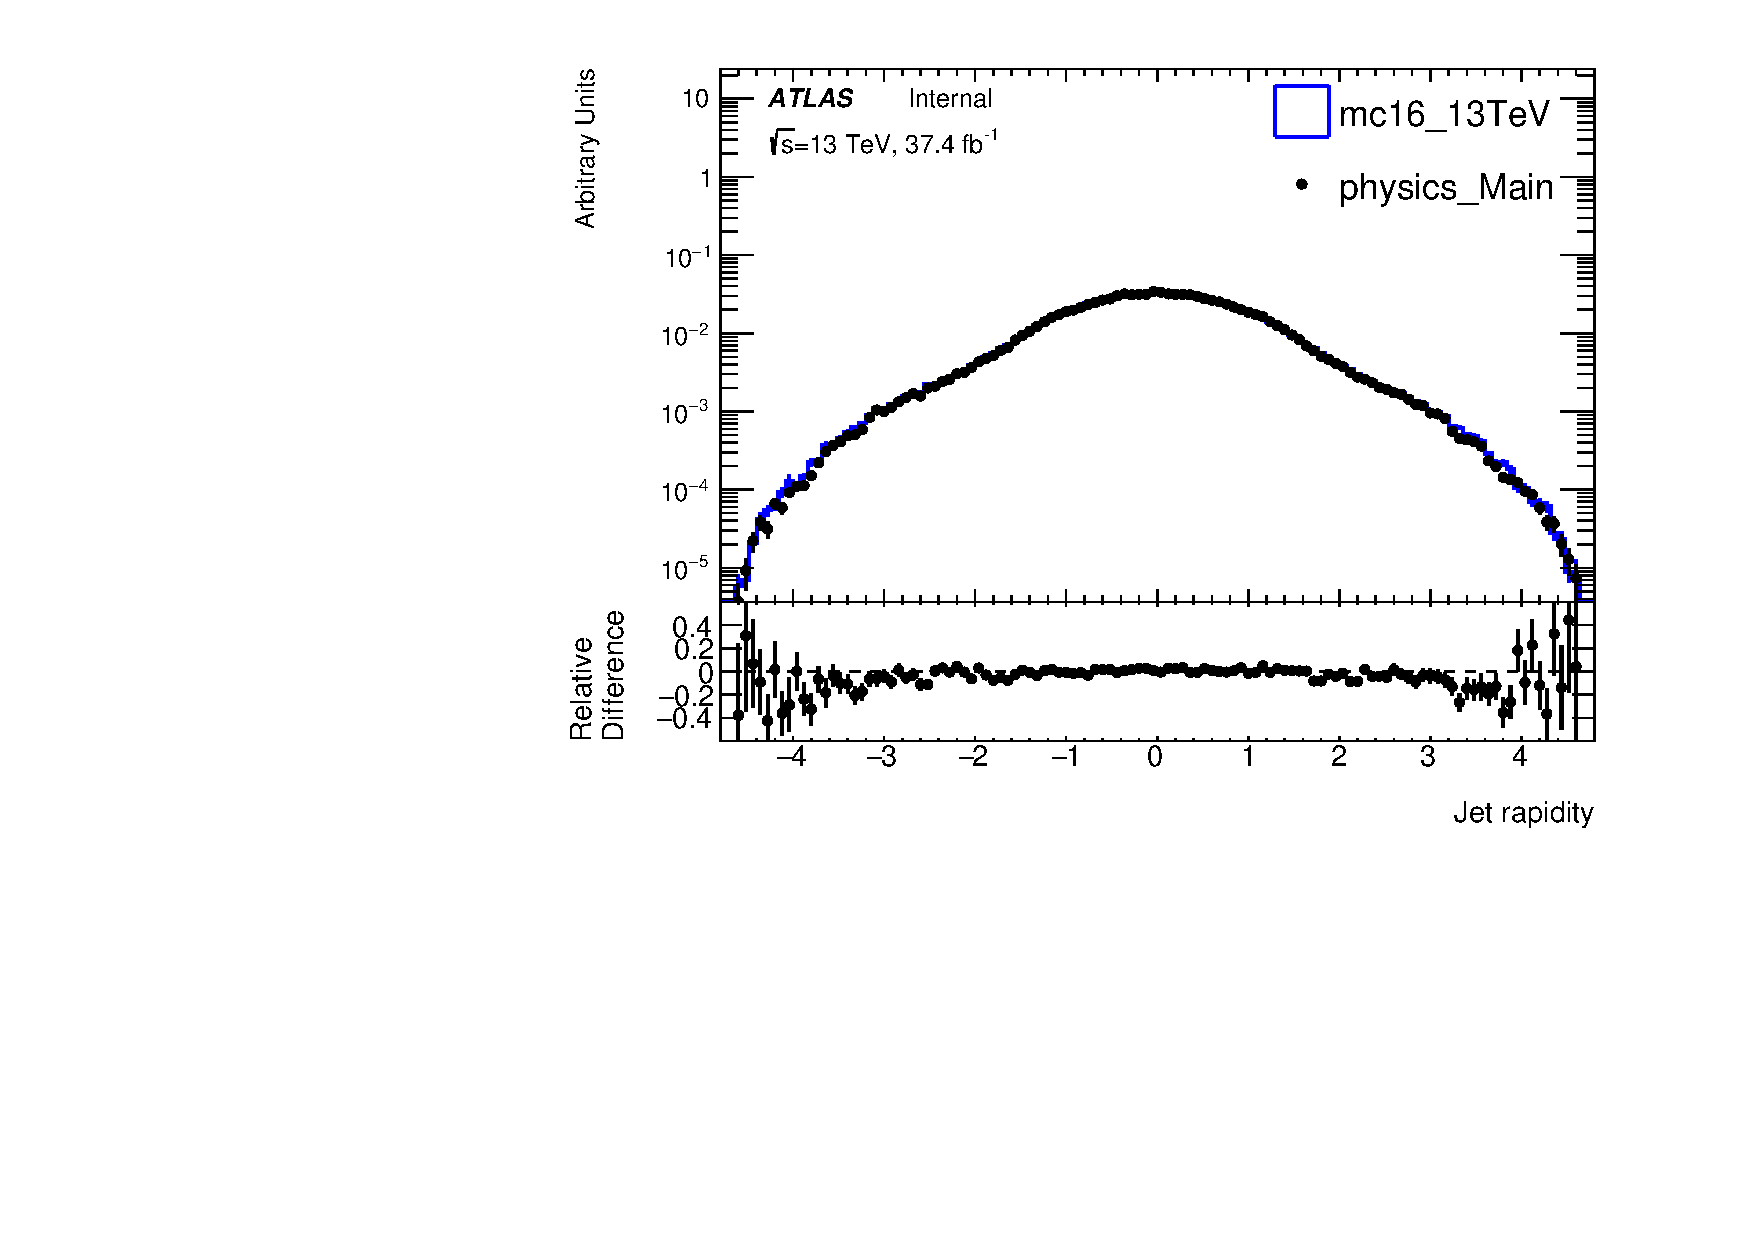
\includegraphics[width=0.45\textwidth]{figures/monitoring/resonant/2015-16/QQ/newStudy_jet_rapidity_logY_QQv01.pdf}}
 %
 
  \caption{Jet plots on %2016 data, 
  the resonant selection. (a) number of jets (b) $\Delta\phi$ between the two jets (c) jet $\eta$
  (d) jet $\phi$ (e) jet \pt\ (f) jet rapidity.  Fluctuations in the jet $phi$ distribution are attributable to dead modules in the tile calorimeter which lead to fewer jets in small slices of the detector.}
 \label{fig:QQmonitoring5}
\end{figure}


 \begin{figure}[htb]
 \centering
 %
 \subfigure[] {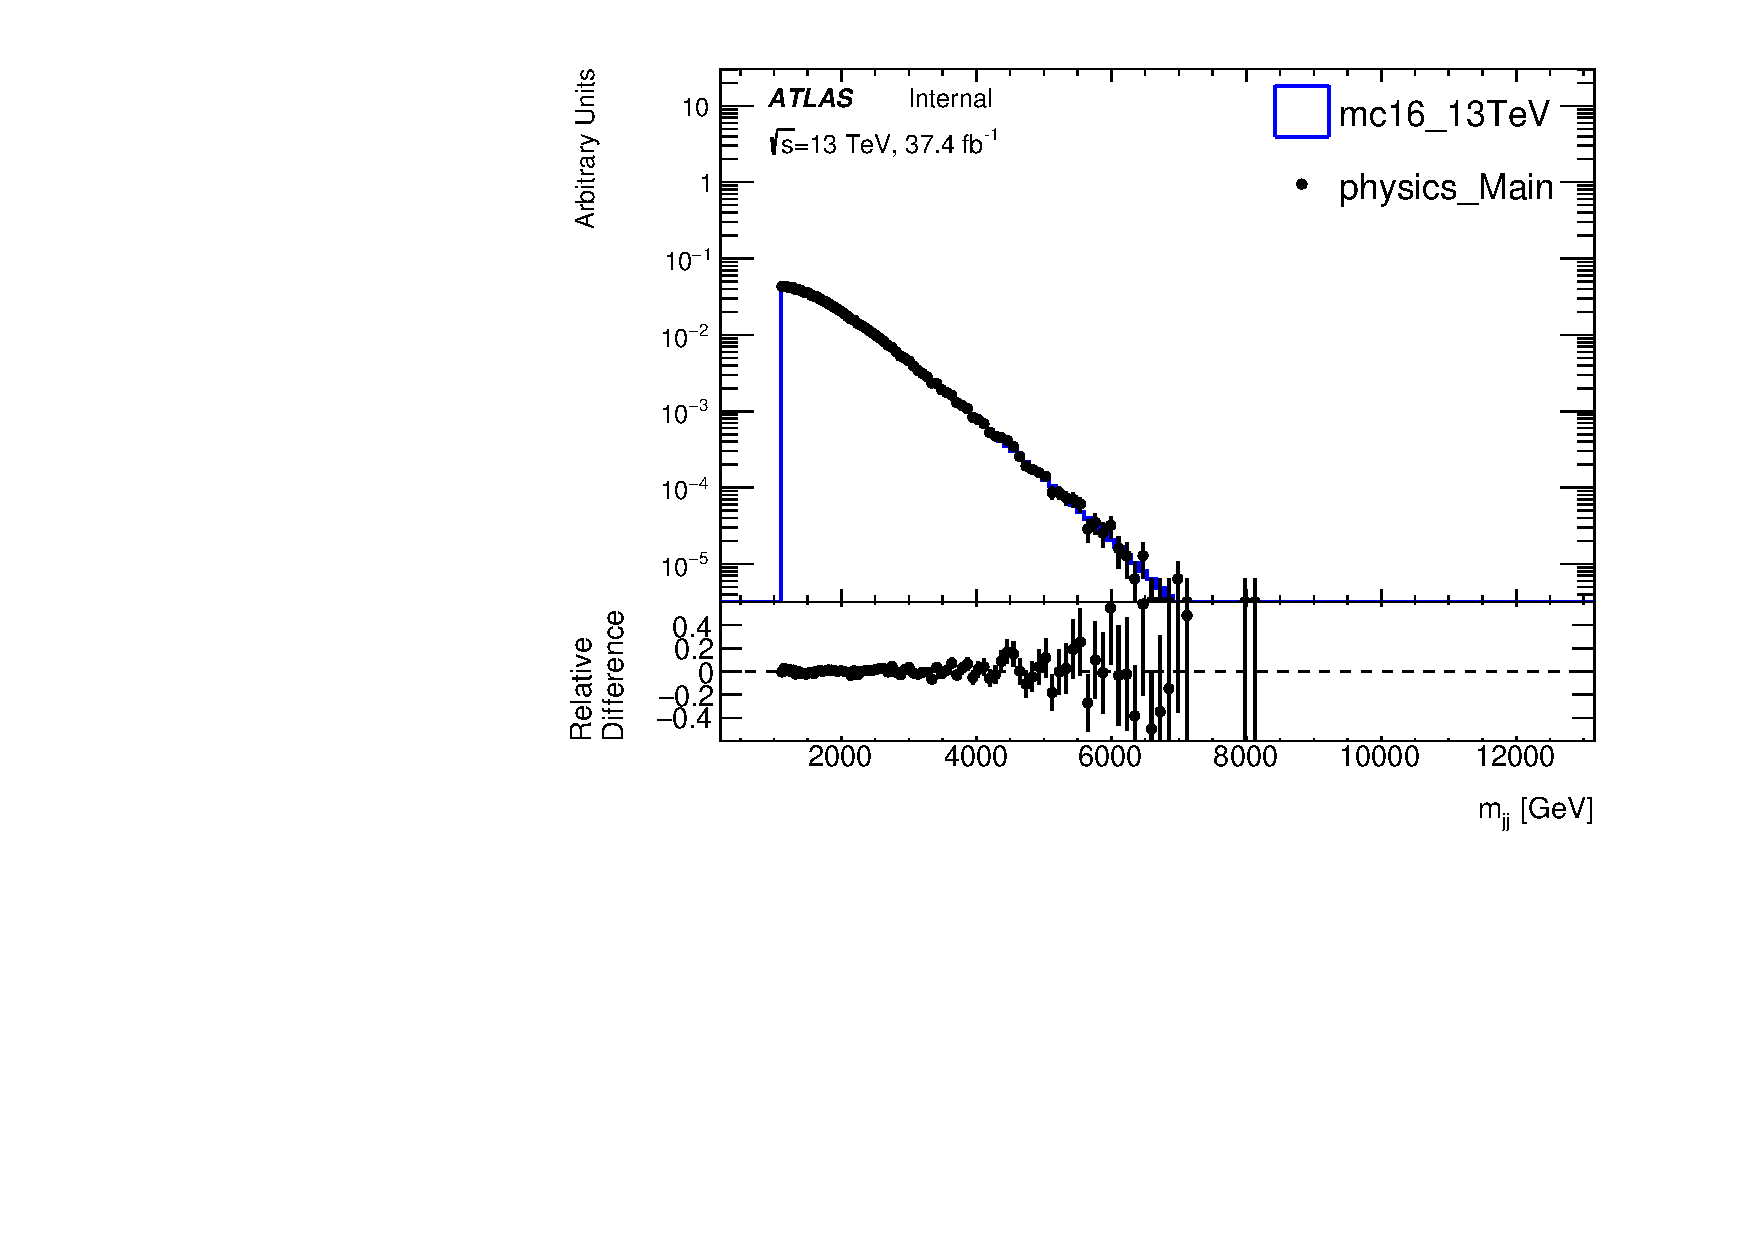
\includegraphics[width=0.45\textwidth]{figures/monitoring/resonant/2015-16/QQ/newStudy_mjj_logY_QQv01.pdf}}
 \subfigure[] {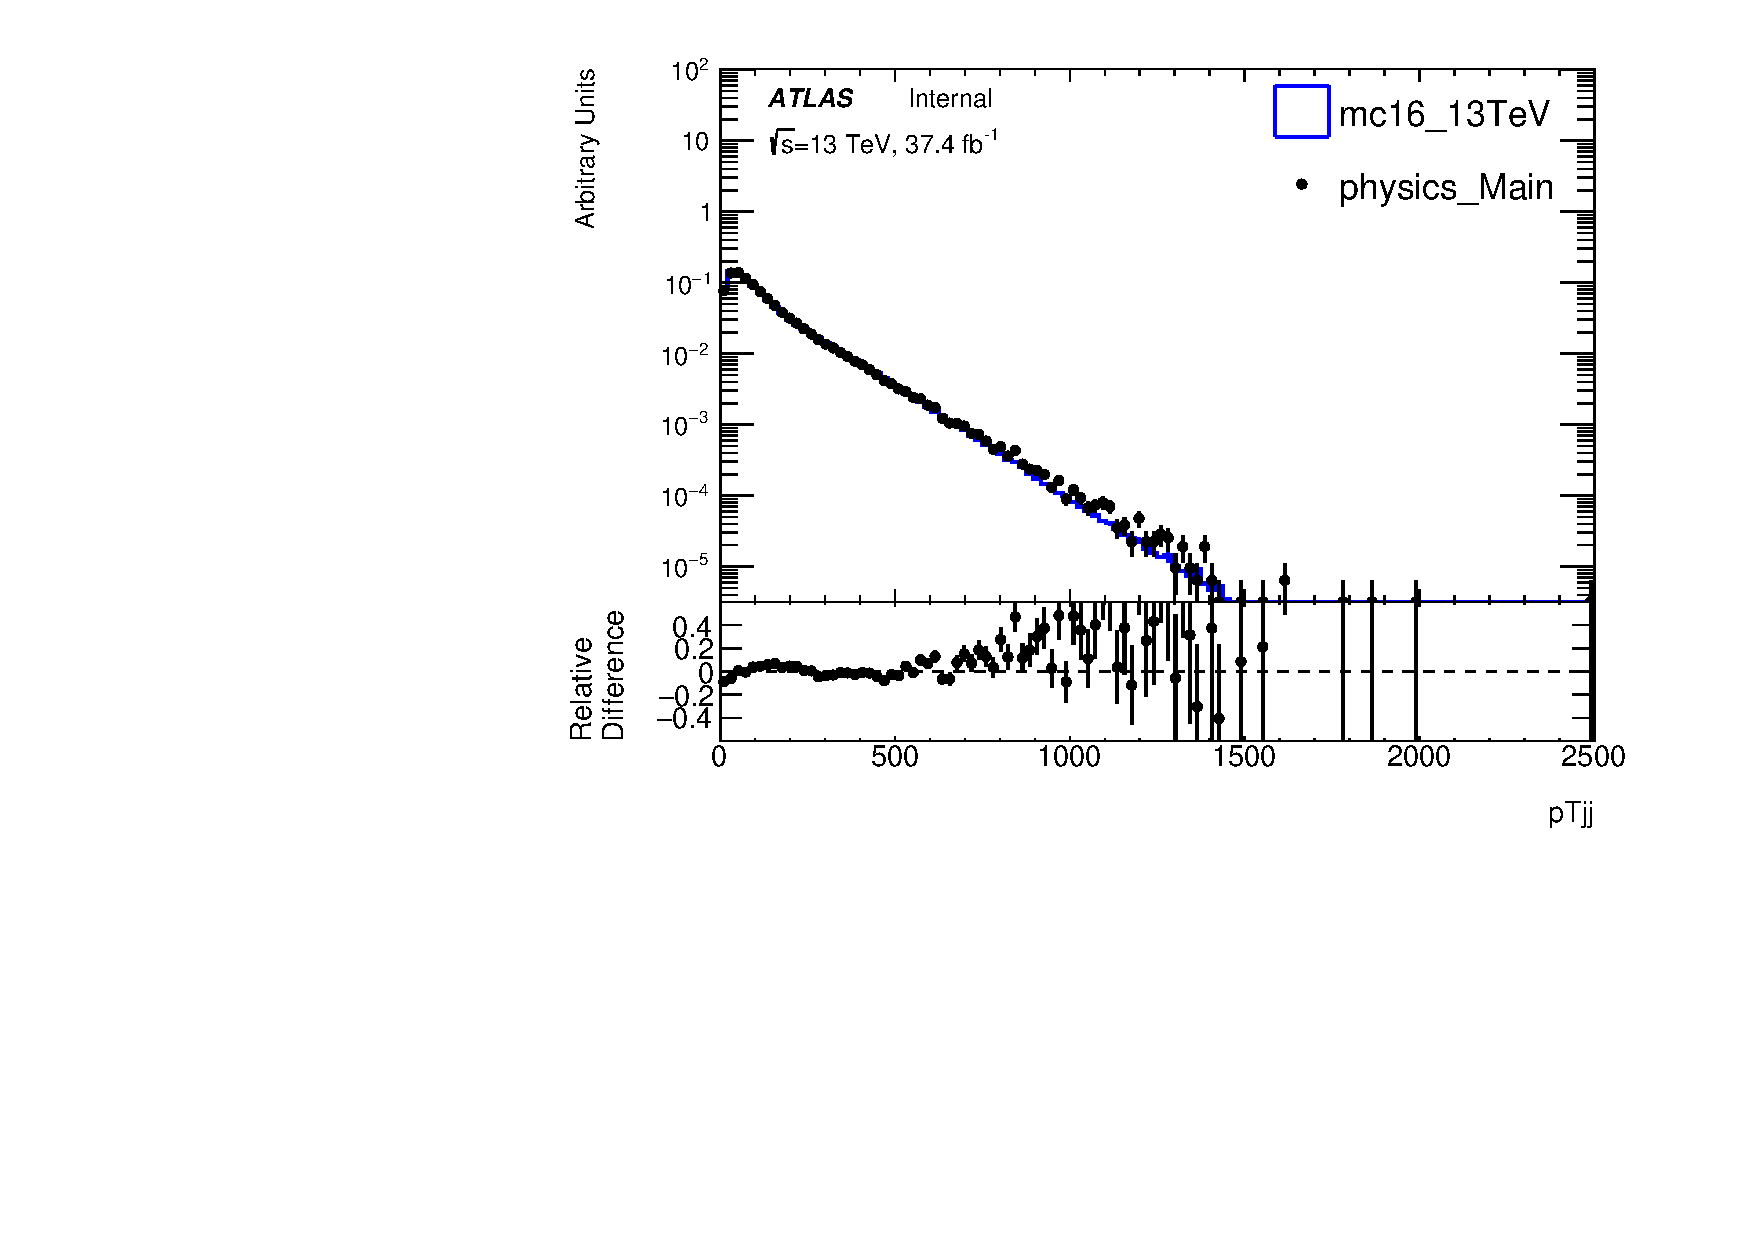
\includegraphics[width=0.45\textwidth]{figures/monitoring/resonant/2015-16/QQ/newStudy_pTjj_logY_QQv01.pdf}}
 %
 \subfigure[] {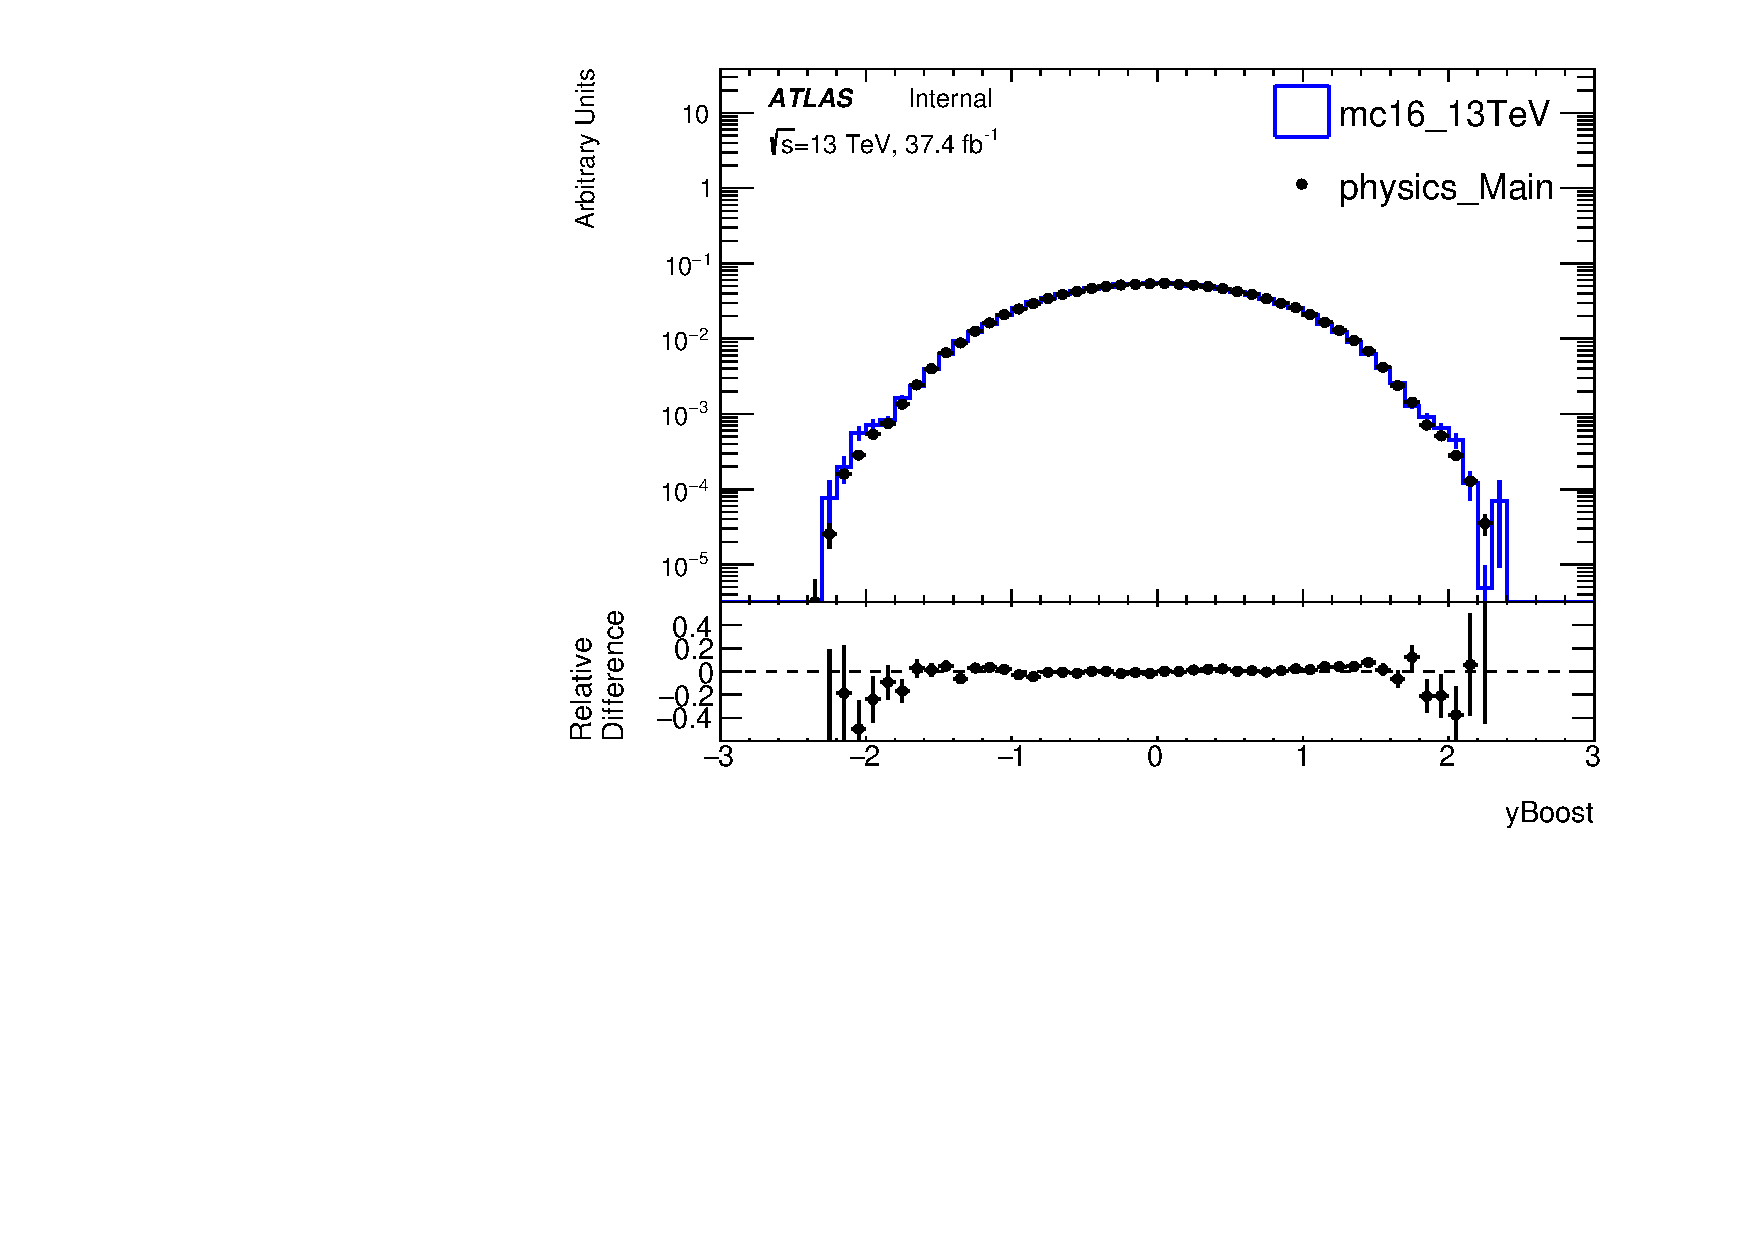
\includegraphics[width=0.45\textwidth]{figures/monitoring/resonant/2015-16/QQ/newStudy_yBoost_logY_QQv01.pdf}}
 \subfigure[] {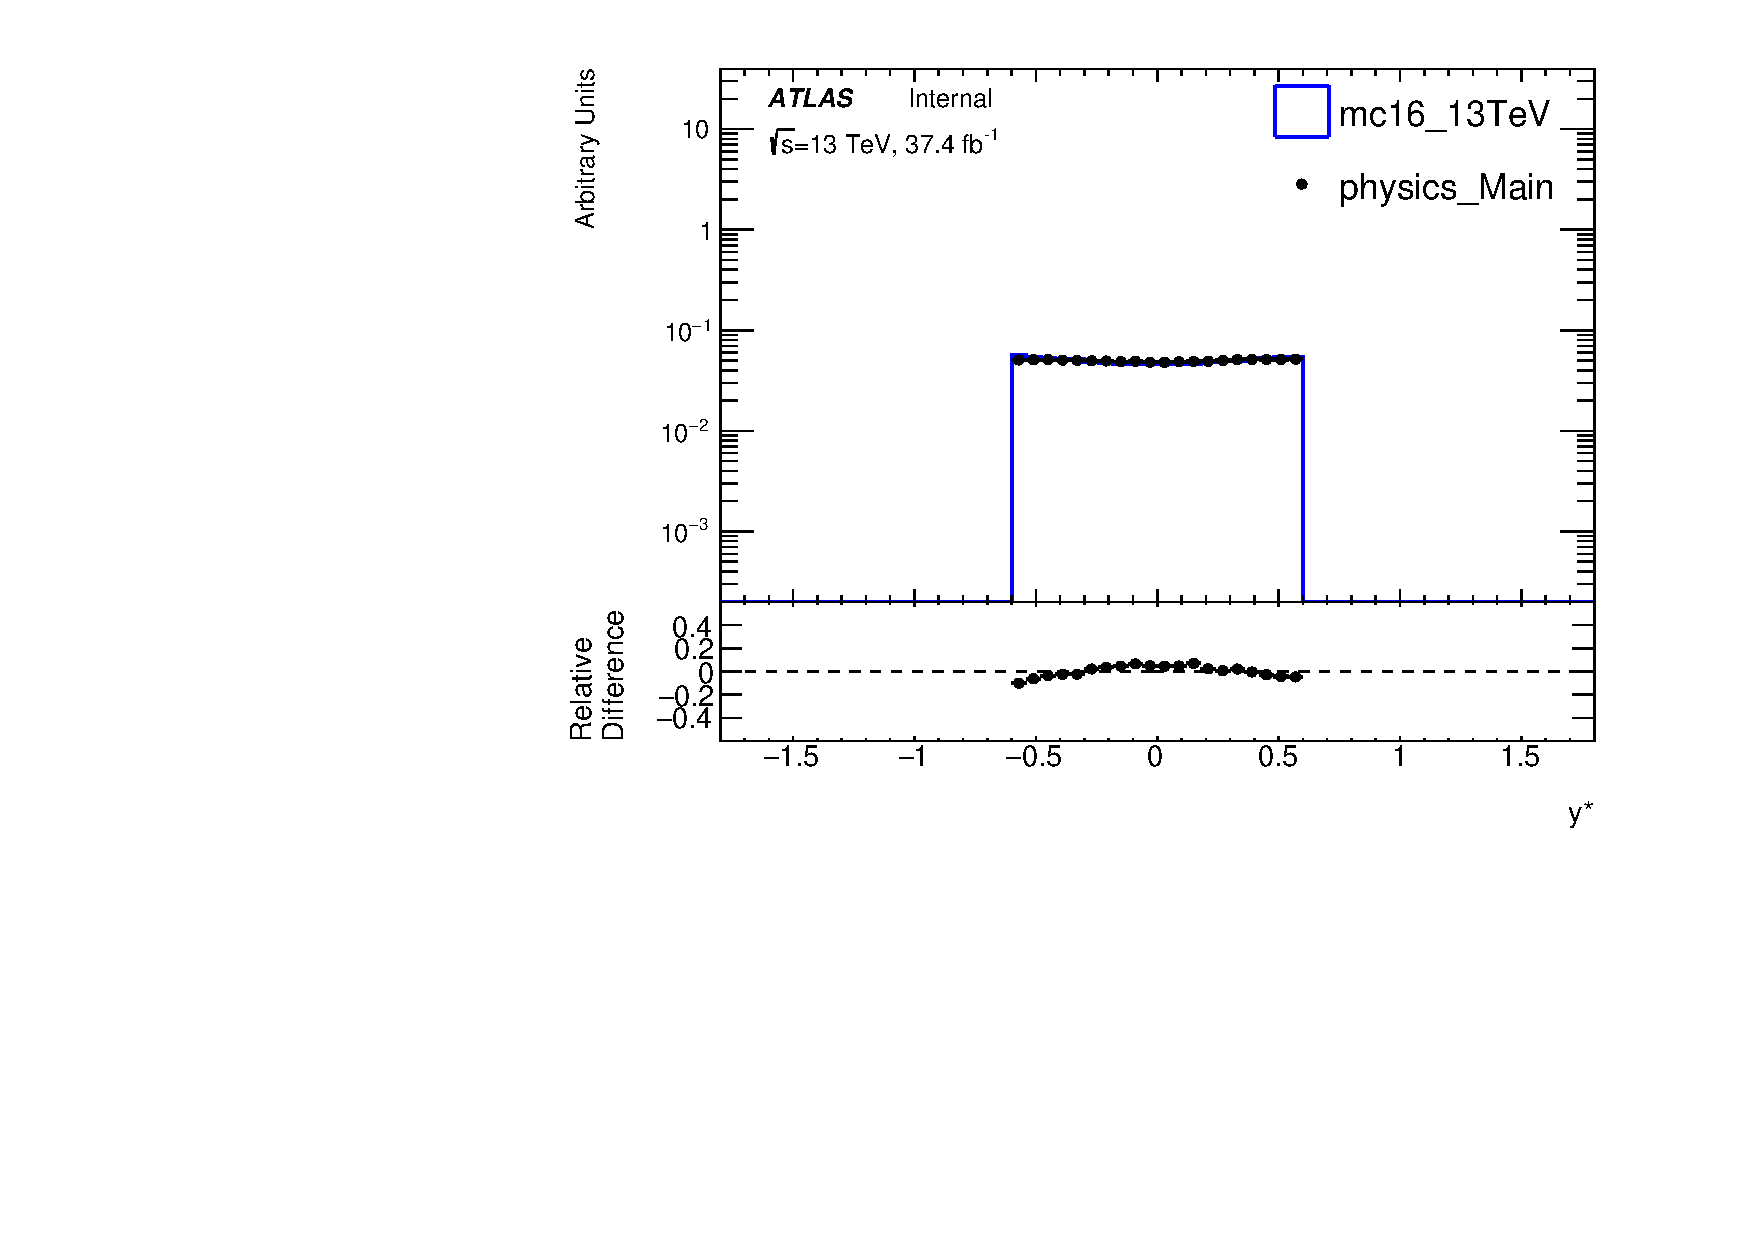
\includegraphics[width=0.45\textwidth]{figures/monitoring/resonant/2015-16/QQ/newStudy_yStar_logY_QQv01.pdf}}
 \caption{Jet plots on %2016 data, 
 the resonant selection. (a) dijet invariant mass (b) dijet \pt\ (c) \yB{} (d) \ystar{}. }
 \label{fig:QQmonitoring6}
\end{figure}

\clearpage

In this section a selection of kinematic and monitoring plots produced with the resonant selection on the QG dataset is shown 
(Figures~\ref{fig:QGmonitoring1},  
\ref{fig:QGmonitoring5}, \ref{fig:QGmonitoring6}). These plots are relative to \integLumi of data collected in 2015 and 2016.
 GRL has been applied here.

\begin{figure}[htb]
 \centering
 \subfigure[] {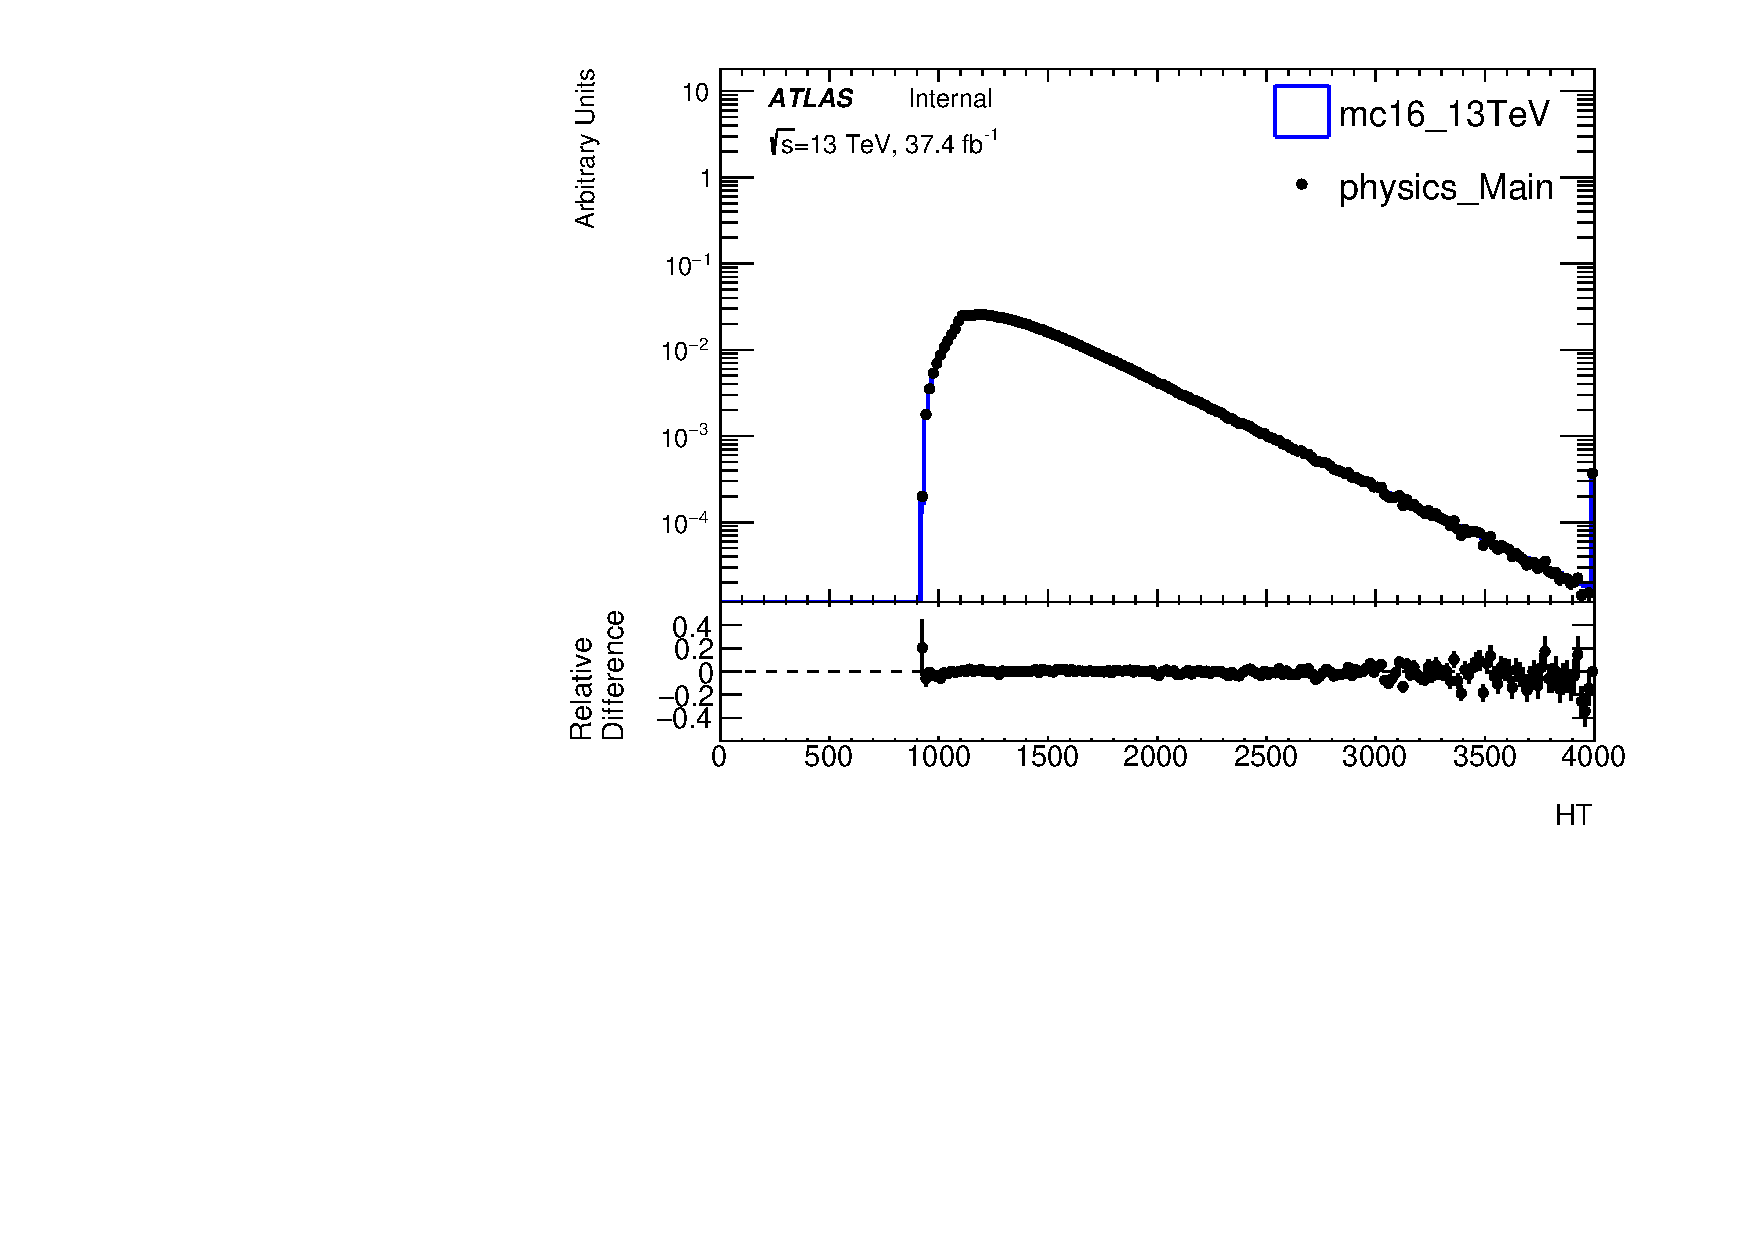
\includegraphics[width=0.45\textwidth]{figures/monitoring/resonant/2015-16/QG/newStudy_HT_logY_QGv01.pdf}}
 \subfigure[] {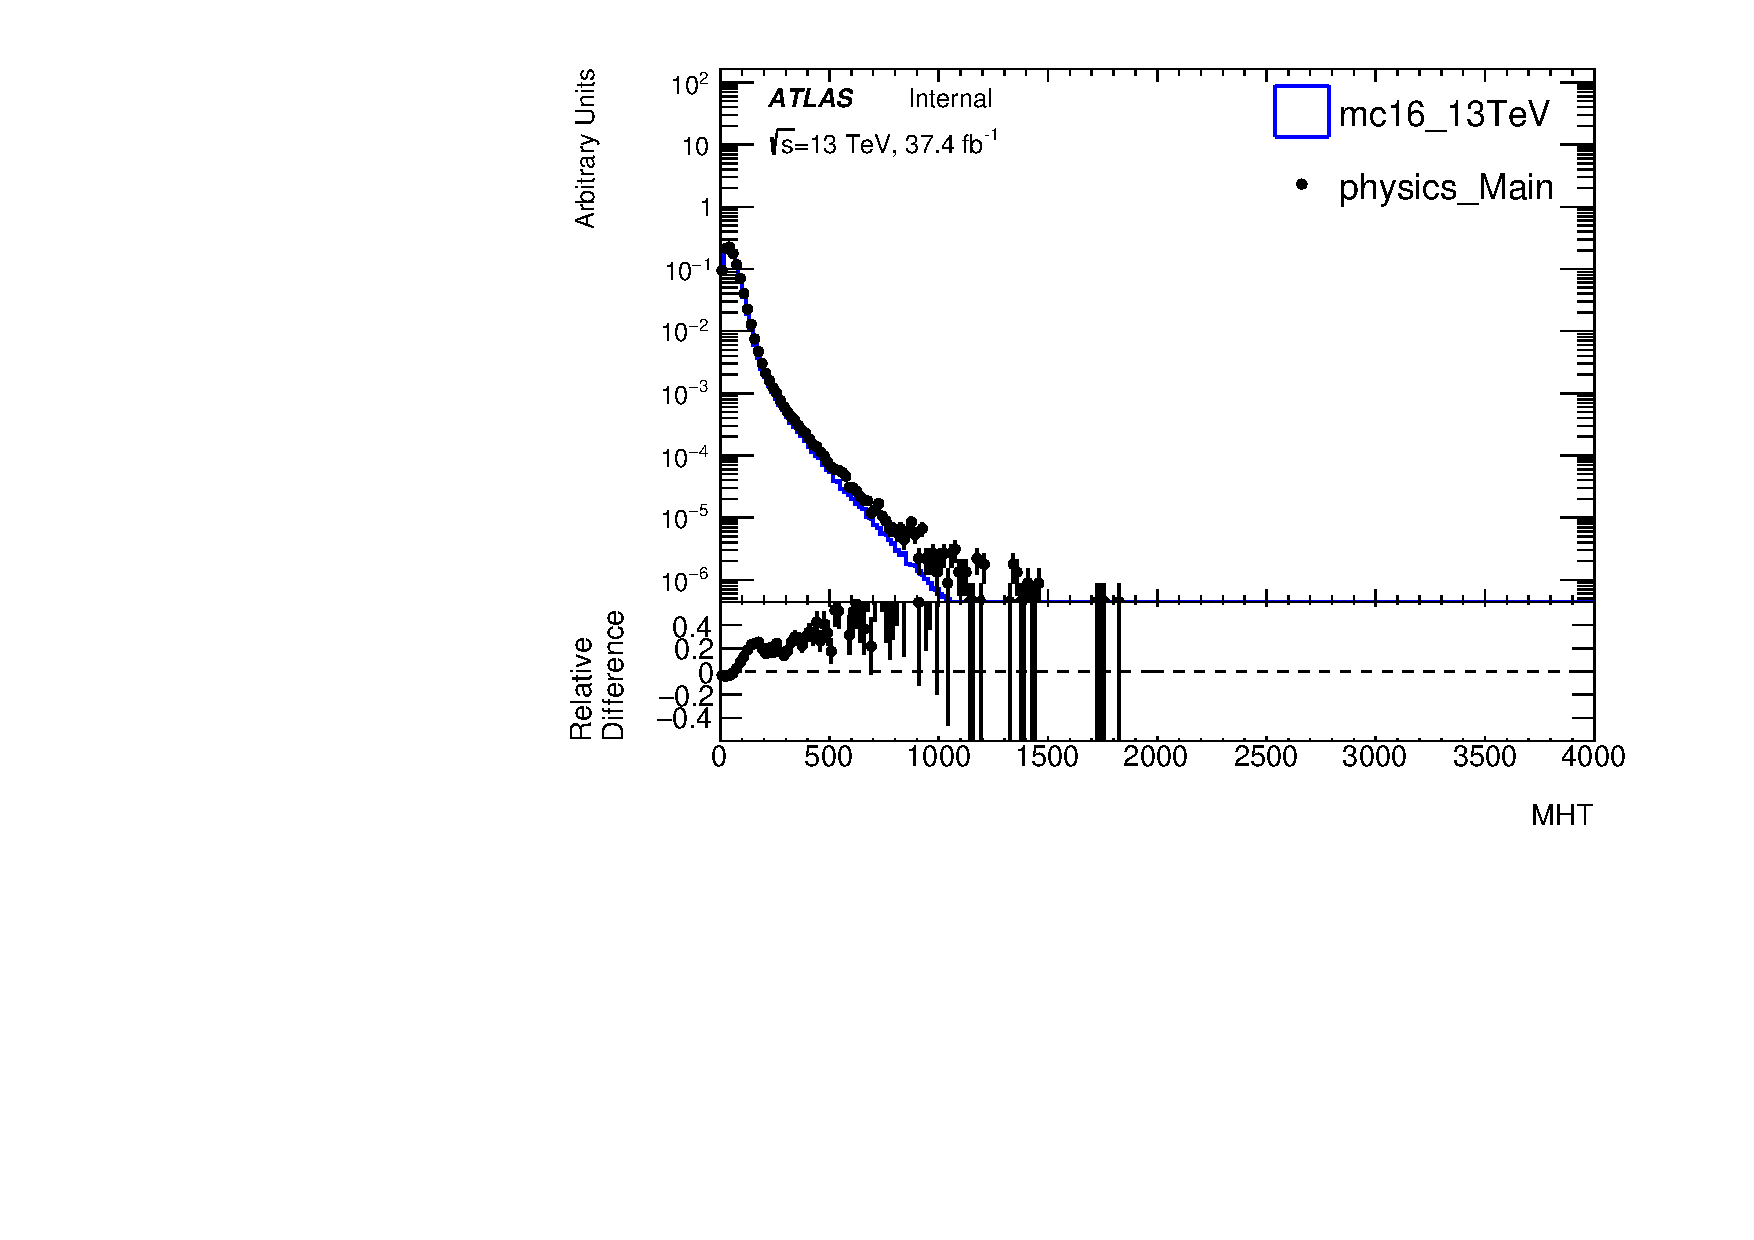
\includegraphics[width=0.45\textwidth]{figures/monitoring/resonant/2015-16/QG/newStudy_MHT_logY_QGv01.pdf}}
 %
 \subfigure[] {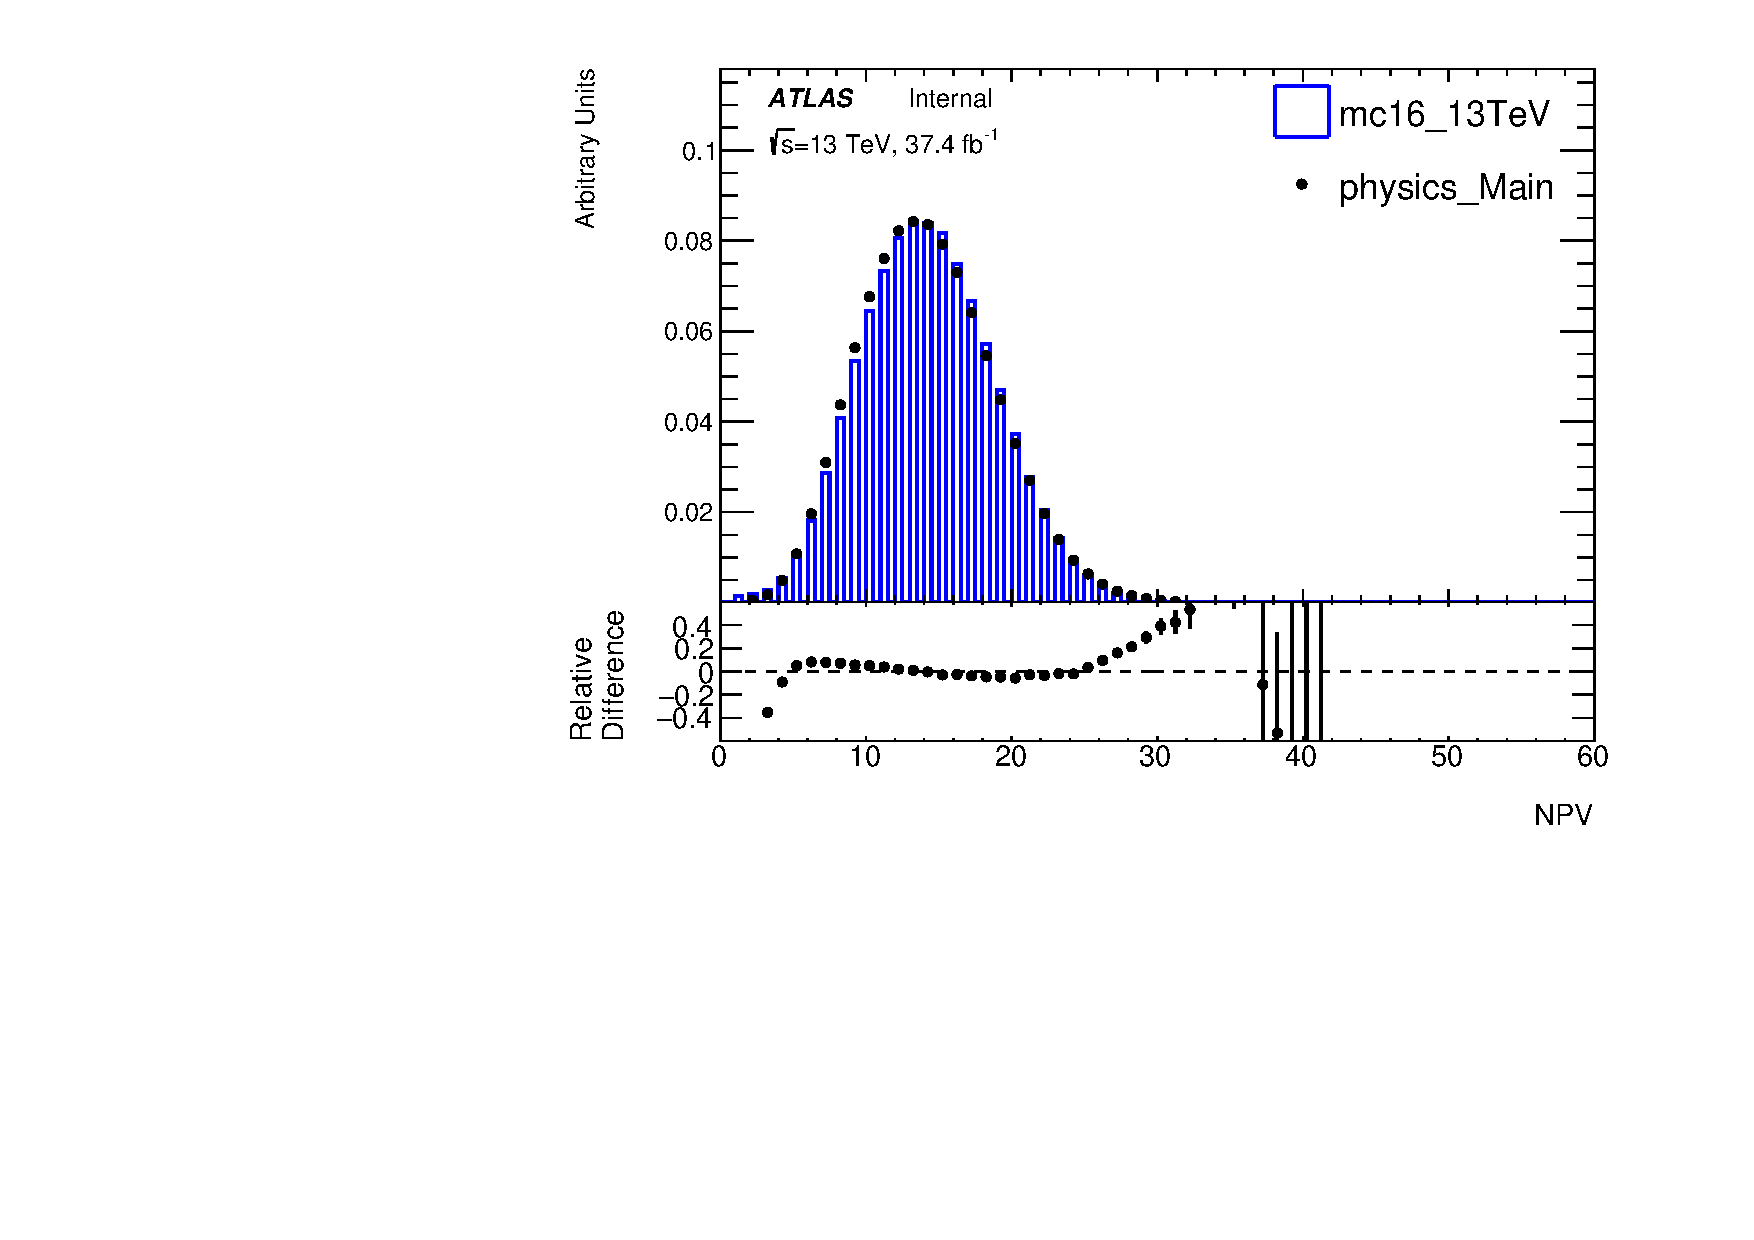
\includegraphics[width=0.45\textwidth]{figures/monitoring/resonant/2015-16/QG/newStudy_NPV_QGv01.pdf}}
 \subfigure[] {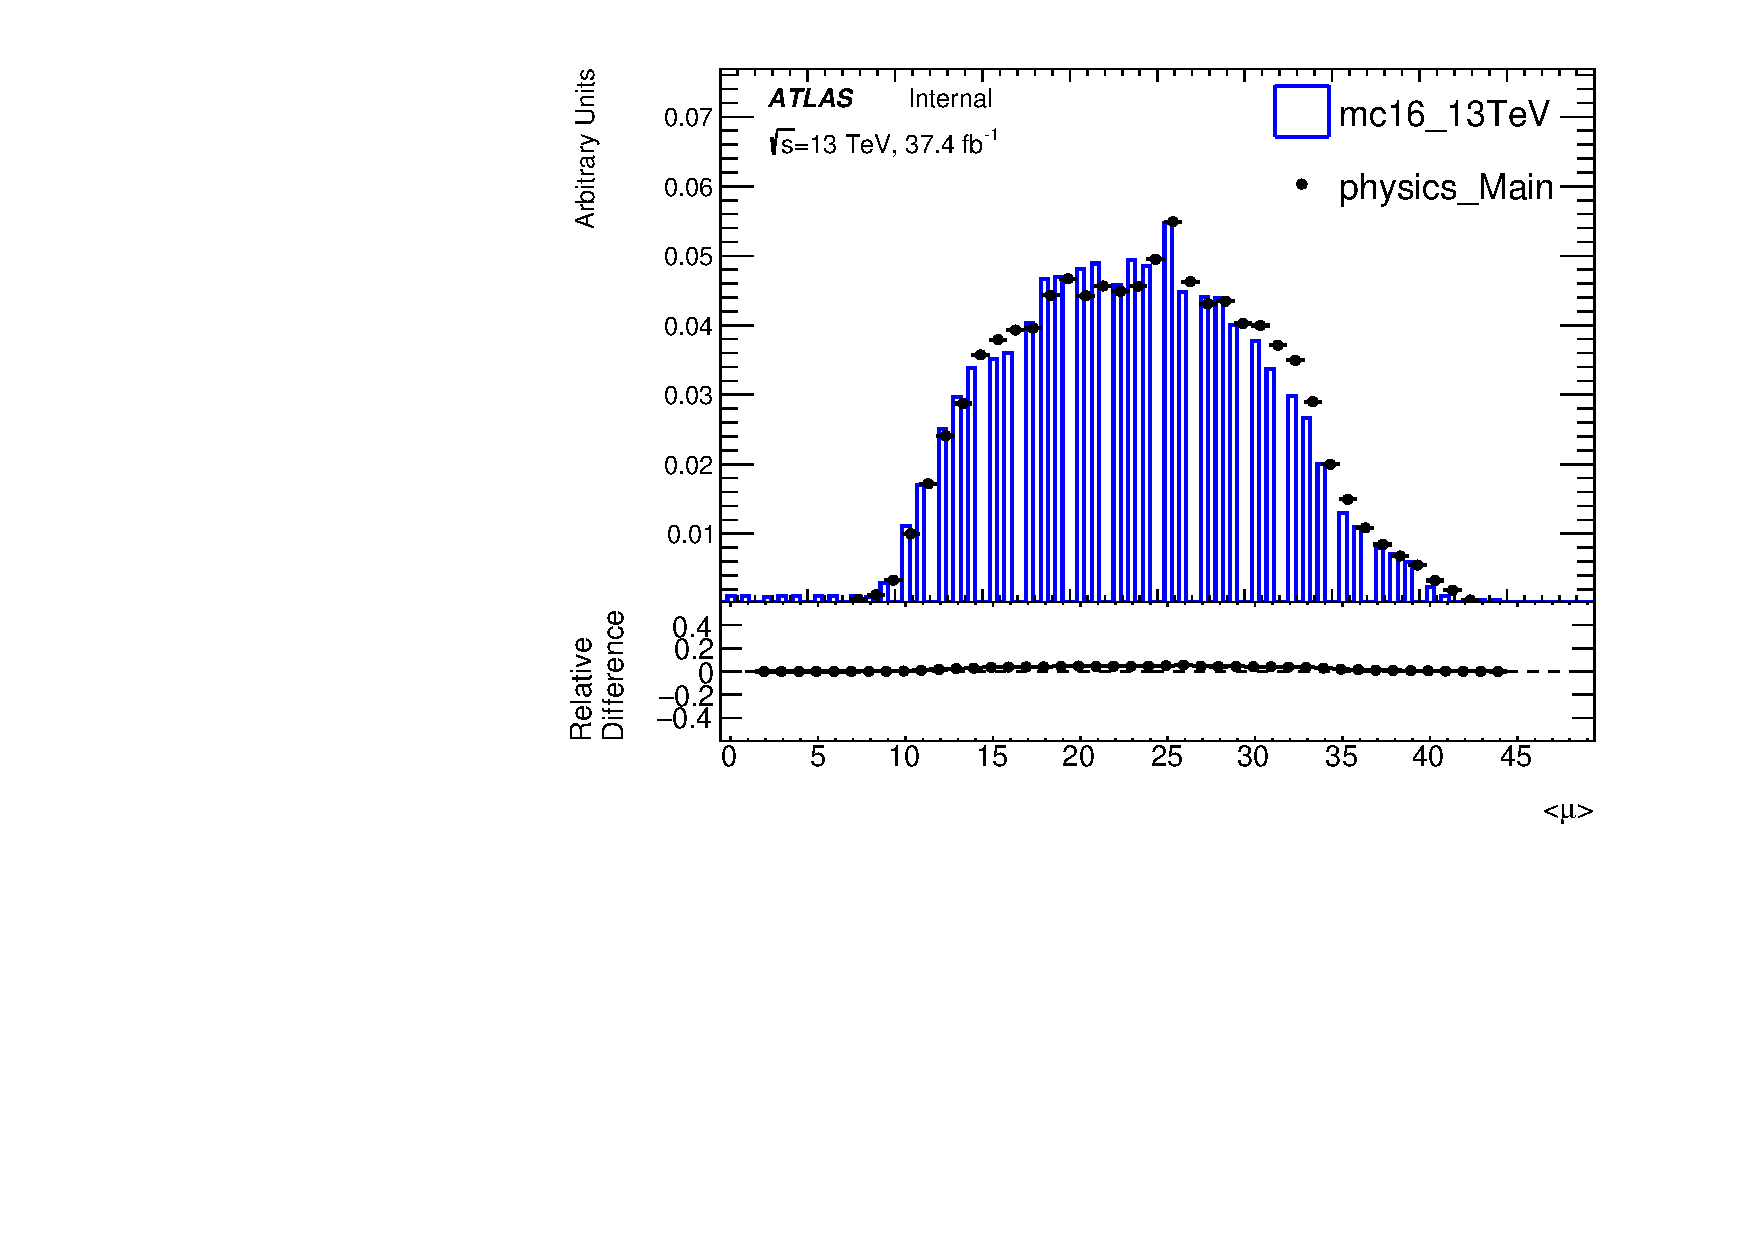
\includegraphics[width=0.45\textwidth]{figures/monitoring/resonant/2015-16/QG/newStudy_averageInteractionsPerCrossing_QGv01.pdf}}
 %

 \caption{Monitoring plots on %2016 data, 
 the QG resonant selection. (a) $H_T$, (b) $MH_T$ (missing transverse momentum calculated only from the jets in the event), (c) number of primary interaction vertices and (d) average interactions per bunch crossing.}
 \label{fig:QGmonitoring1}
\end{figure}

 \begin{figure}[htb]
 \centering
  \subfigure[] {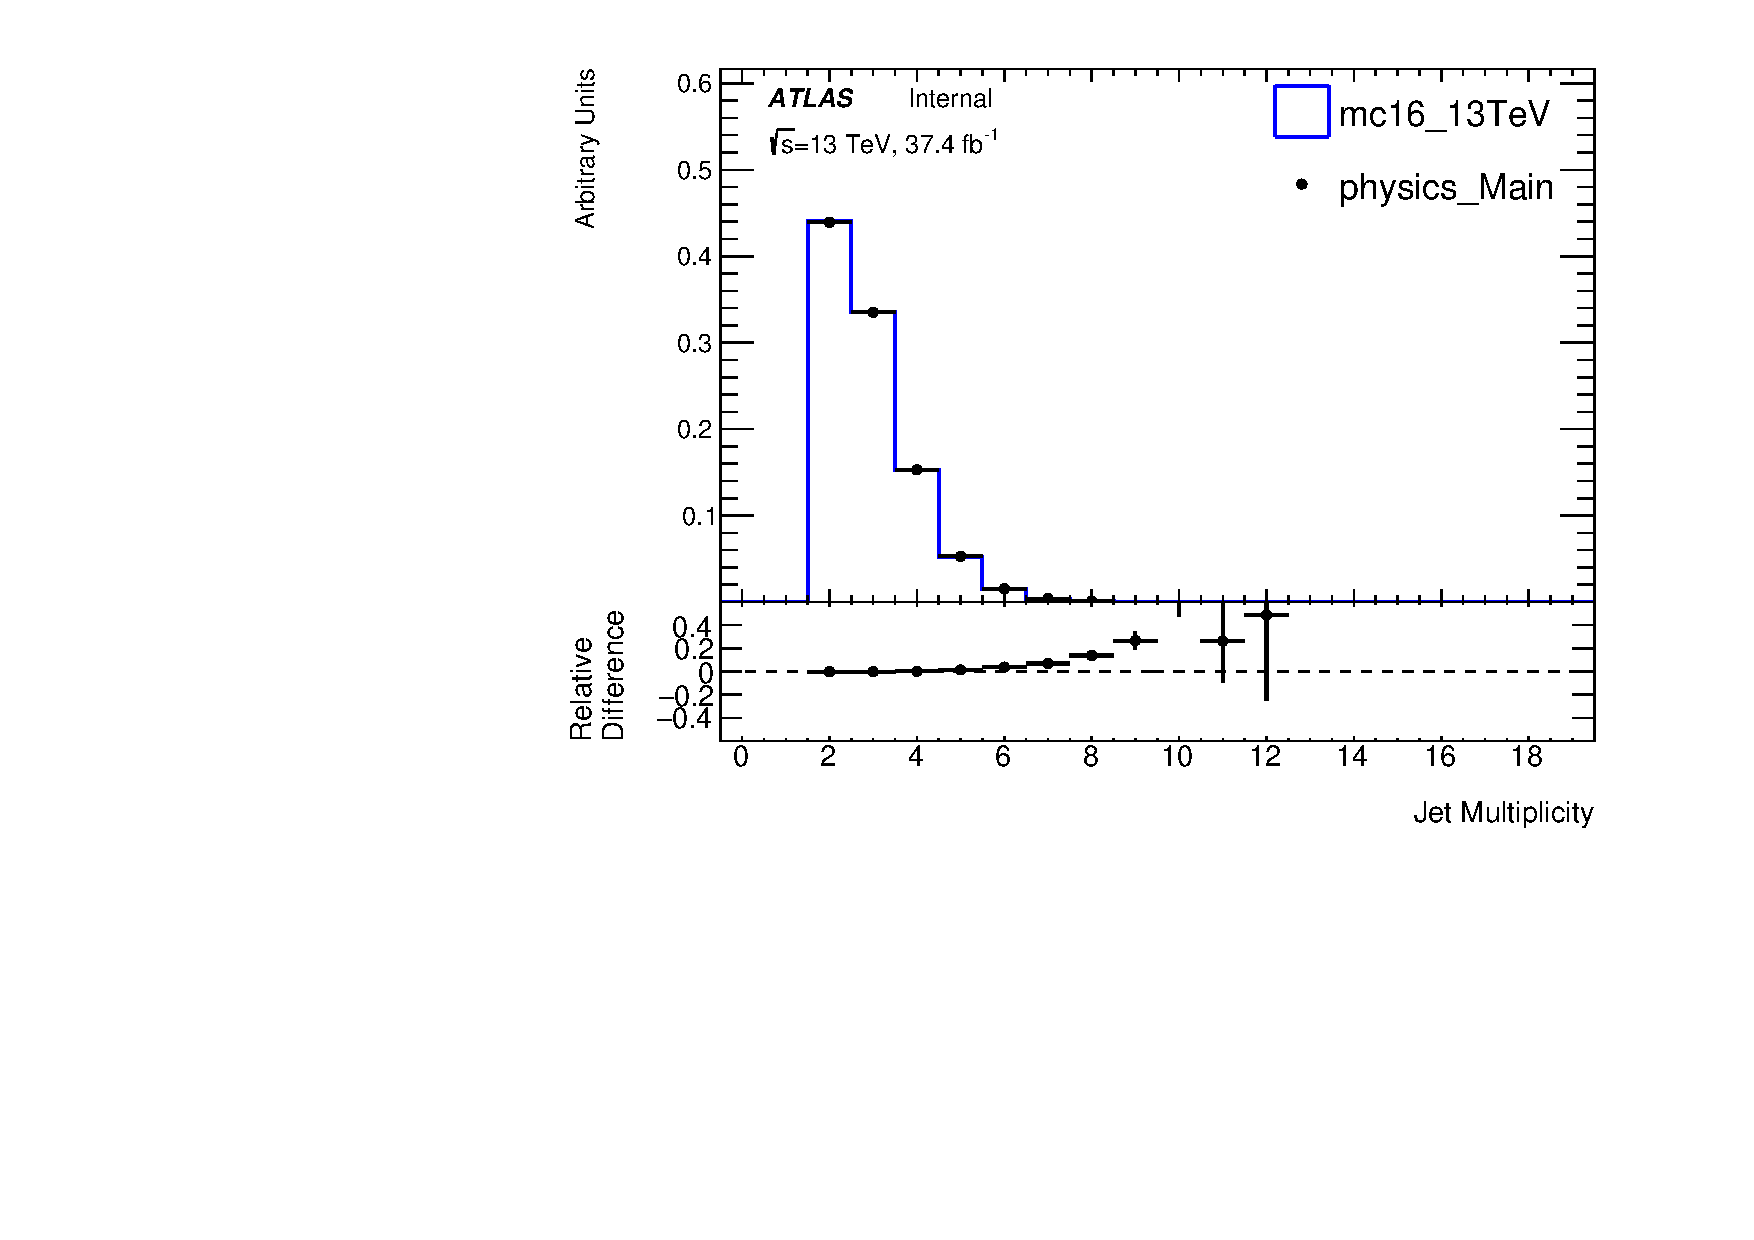
\includegraphics[width=0.45\textwidth]{figures/monitoring/resonant/2015-16/QG/newStudy_njets_QGv01.pdf}}
 \subfigure[] {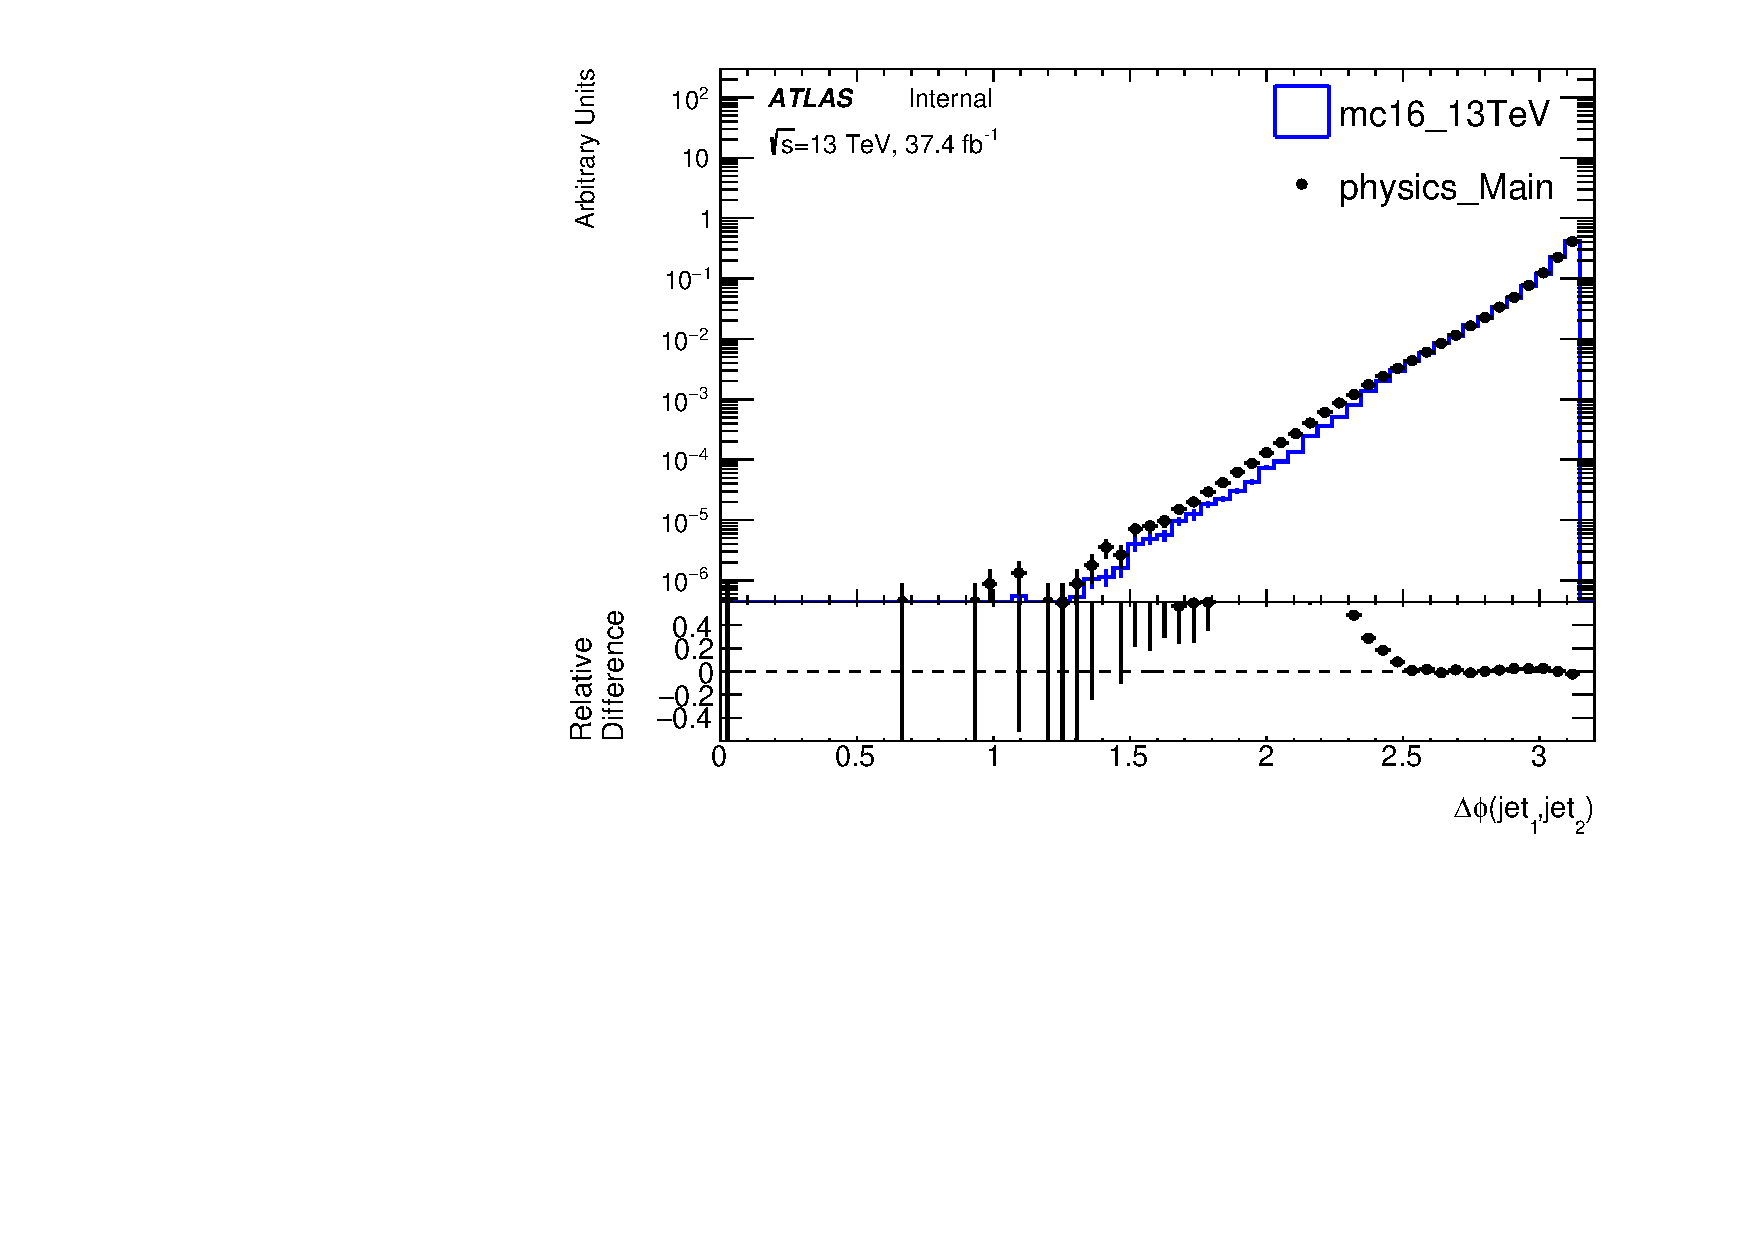
\includegraphics[width=0.45\textwidth]{figures/monitoring/resonant/2015-16/QG//newStudy_deltaPhi_logY_QGv01.pdf}}
 %
 \subfigure[] {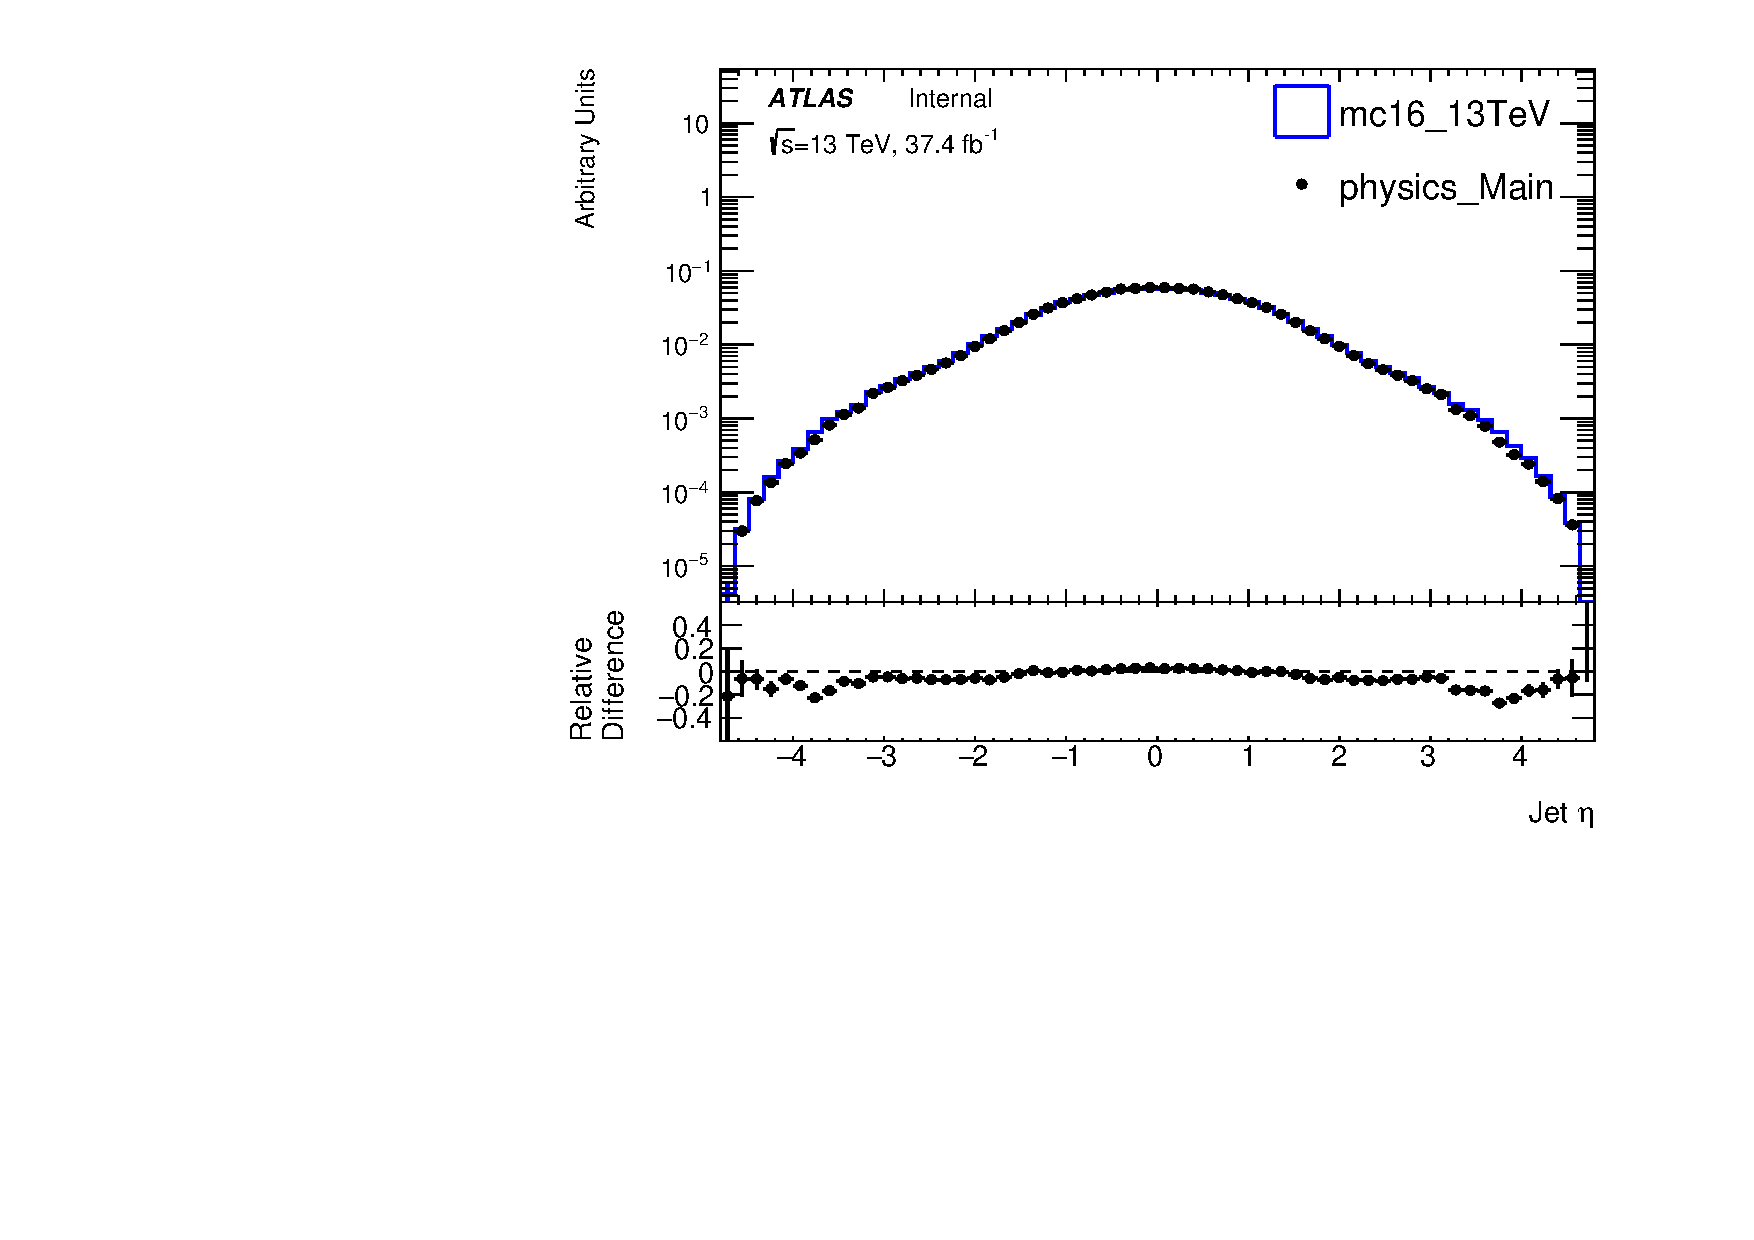
\includegraphics[width=0.45\textwidth]{figures/monitoring/resonant/2015-16/QG/newStudy_jet_eta_logY_QGv01.pdf}}
 \subfigure[] {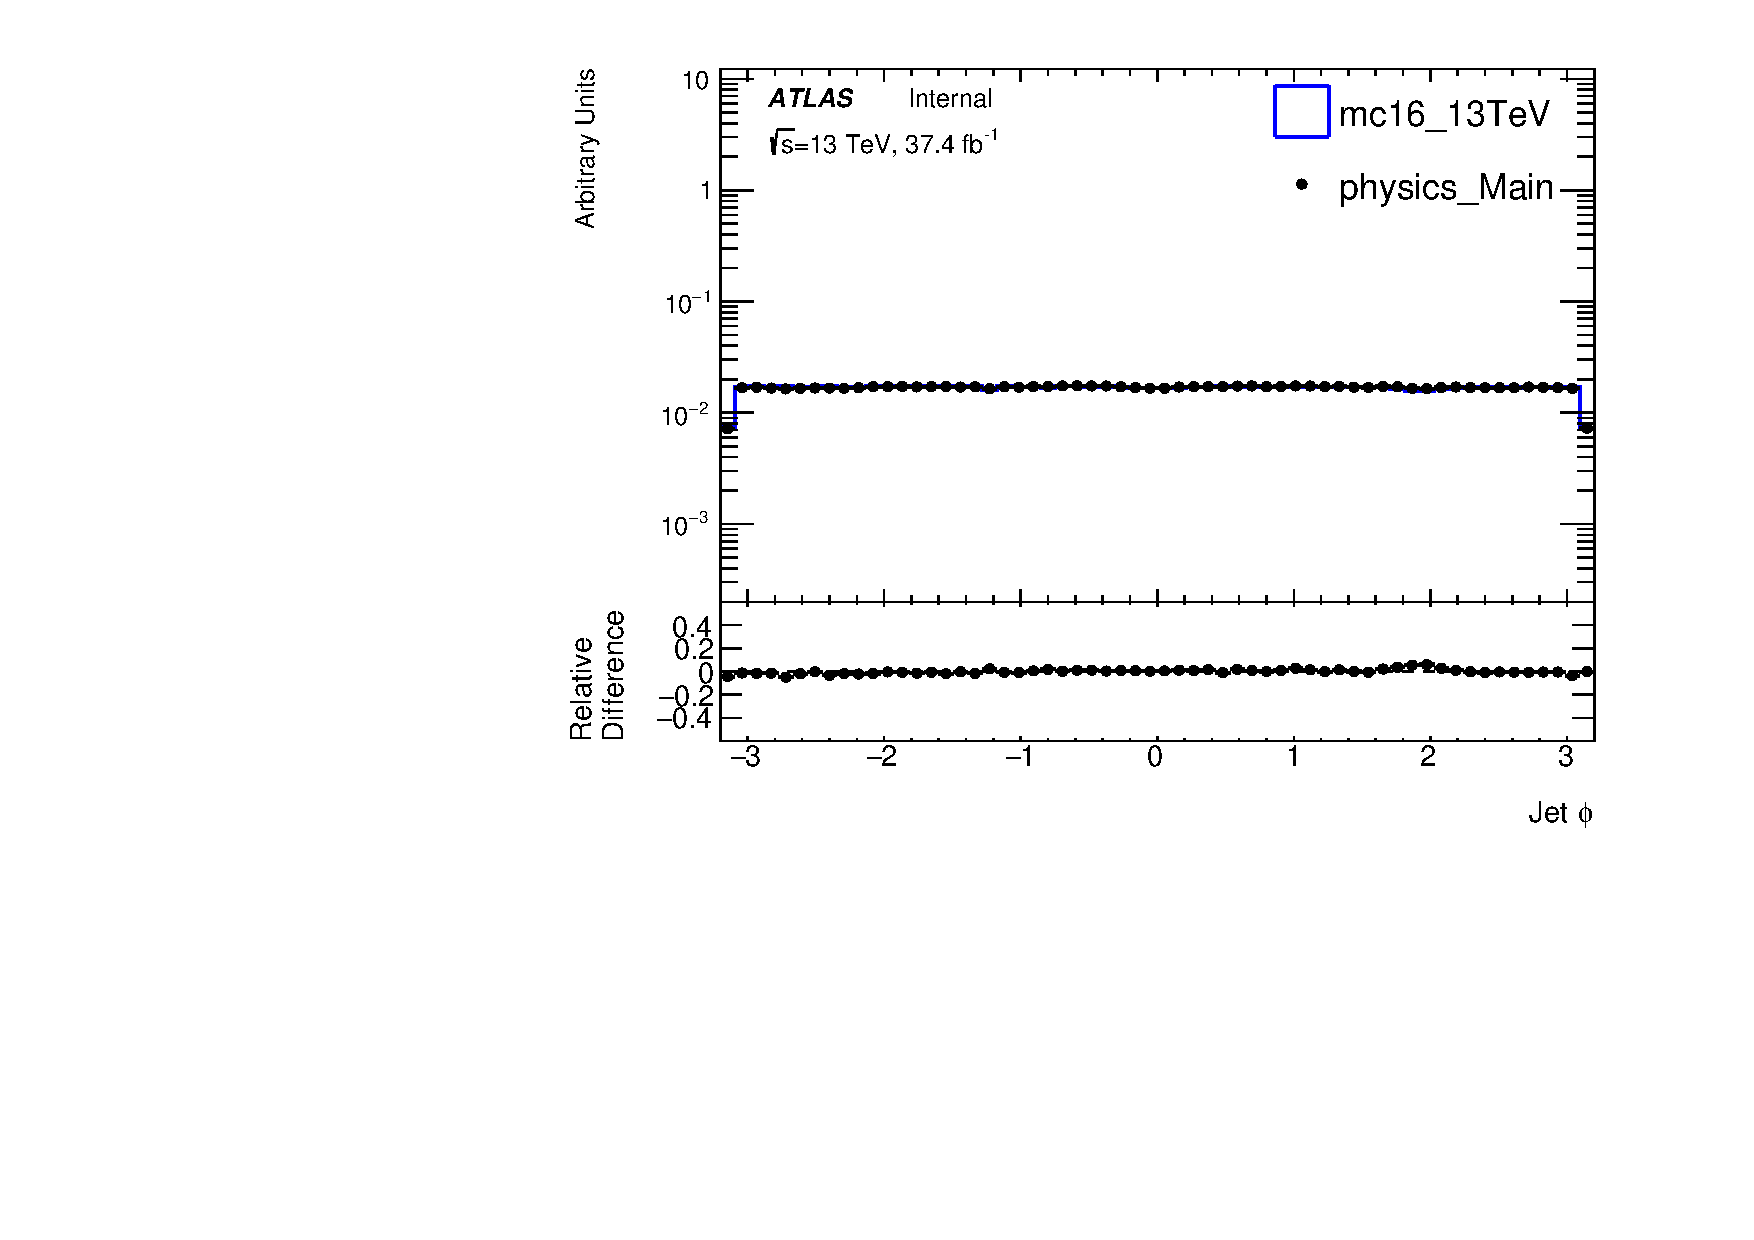
\includegraphics[width=0.45\textwidth]{figures/monitoring/resonant/2015-16/QG/newStudy_jet_phi_logY_QGv01.pdf}}
 %
 \subfigure[] {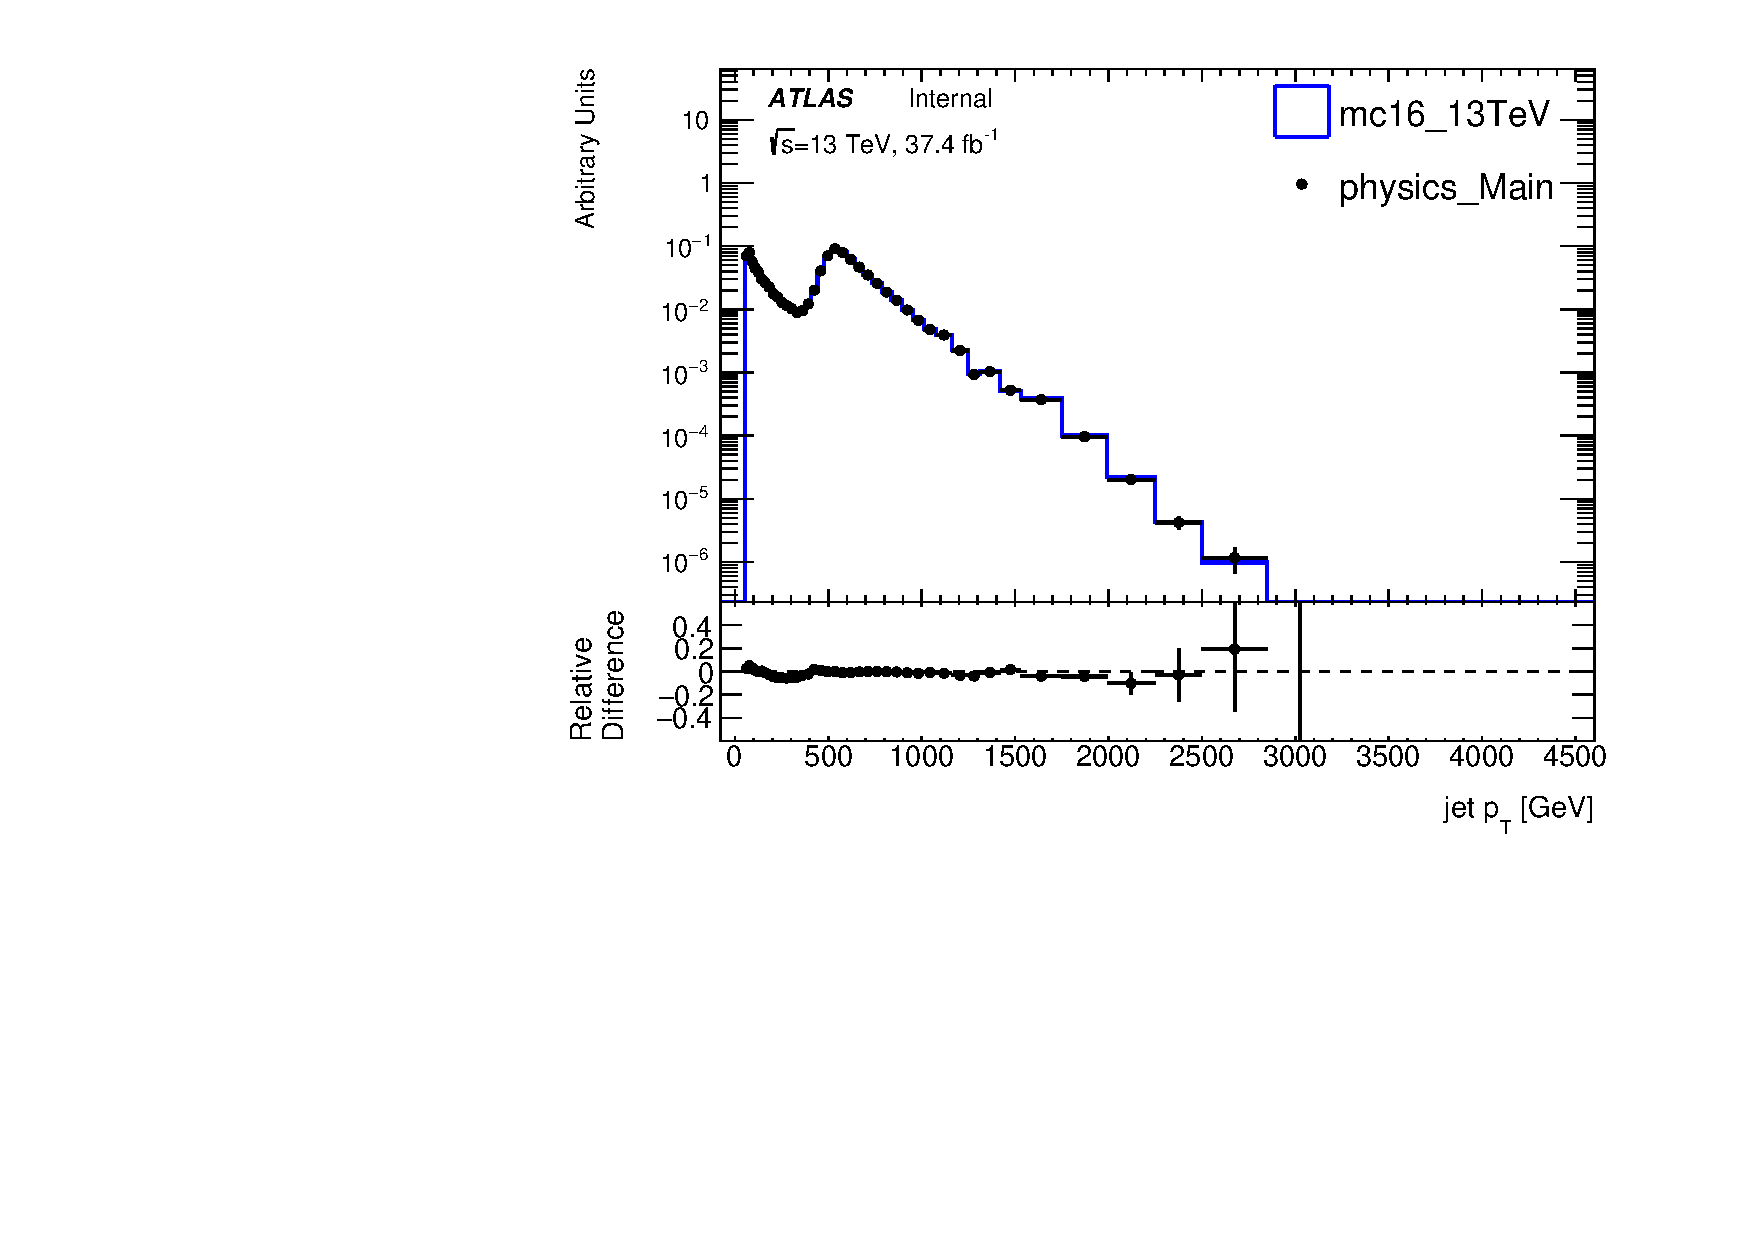
\includegraphics[width=0.45\textwidth]{figures/monitoring/resonant/2015-16/QG/newStudy_jet_pt_logY_QGv01.pdf}}
 \subfigure[] {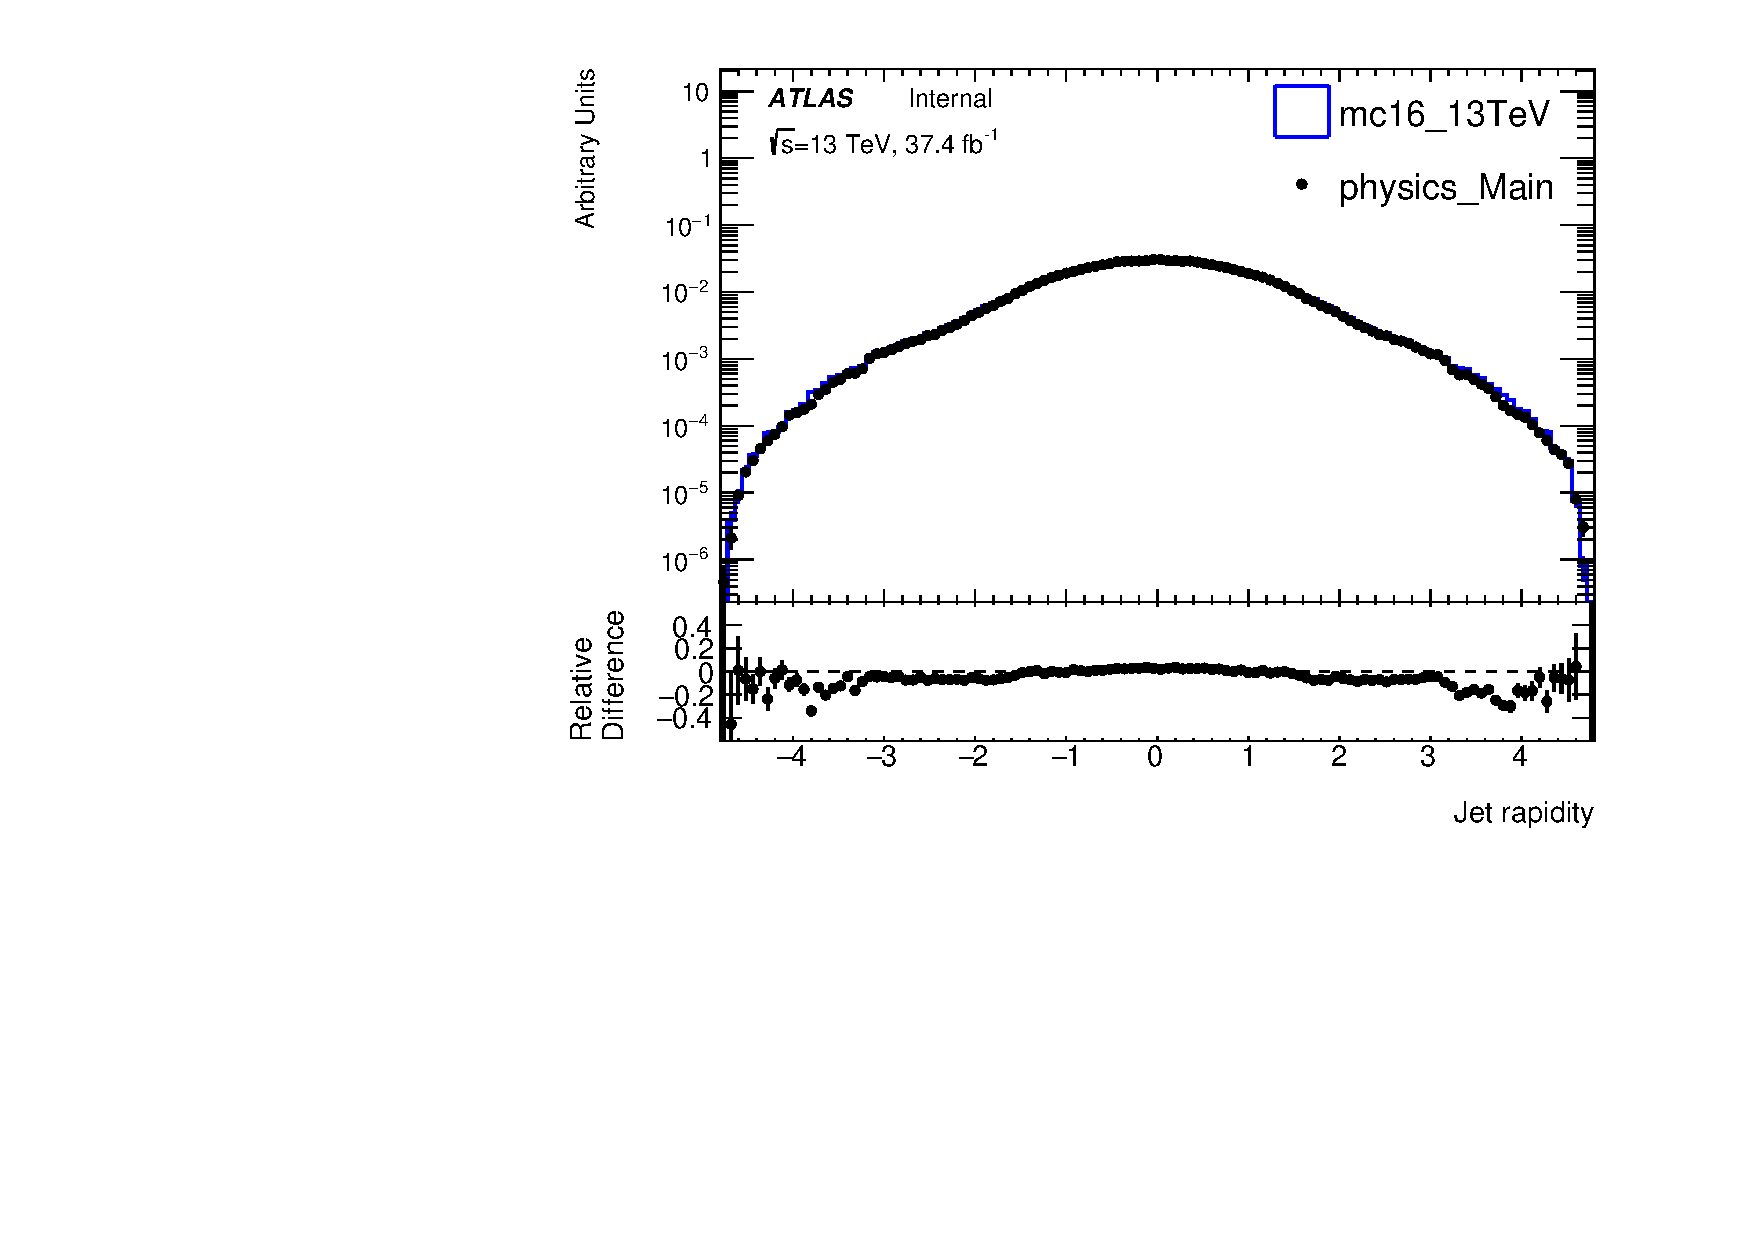
\includegraphics[width=0.45\textwidth]{figures/monitoring/resonant/2015-16/QG/newStudy_jet_rapidity_logY_QGv01.pdf}}
 %
  \caption{Jet plots on %2016 data, 
  the resonant selection. (a) number of jets (b) $\Delta\phi$ between the two jets (c) jet $\eta$
  (d) jet $\phi$ (e) jet \pt\ (f) jet rapidity.  Fluctuations in the jet $phi$ distribution are attributable to dead modules in the tile calorimeter which lead to fewer jets in small slices of the detector.}
 \label{fig:QGmonitoring5}
\end{figure}


 \begin{figure}[htb]
 \centering
 %
 \subfigure[] {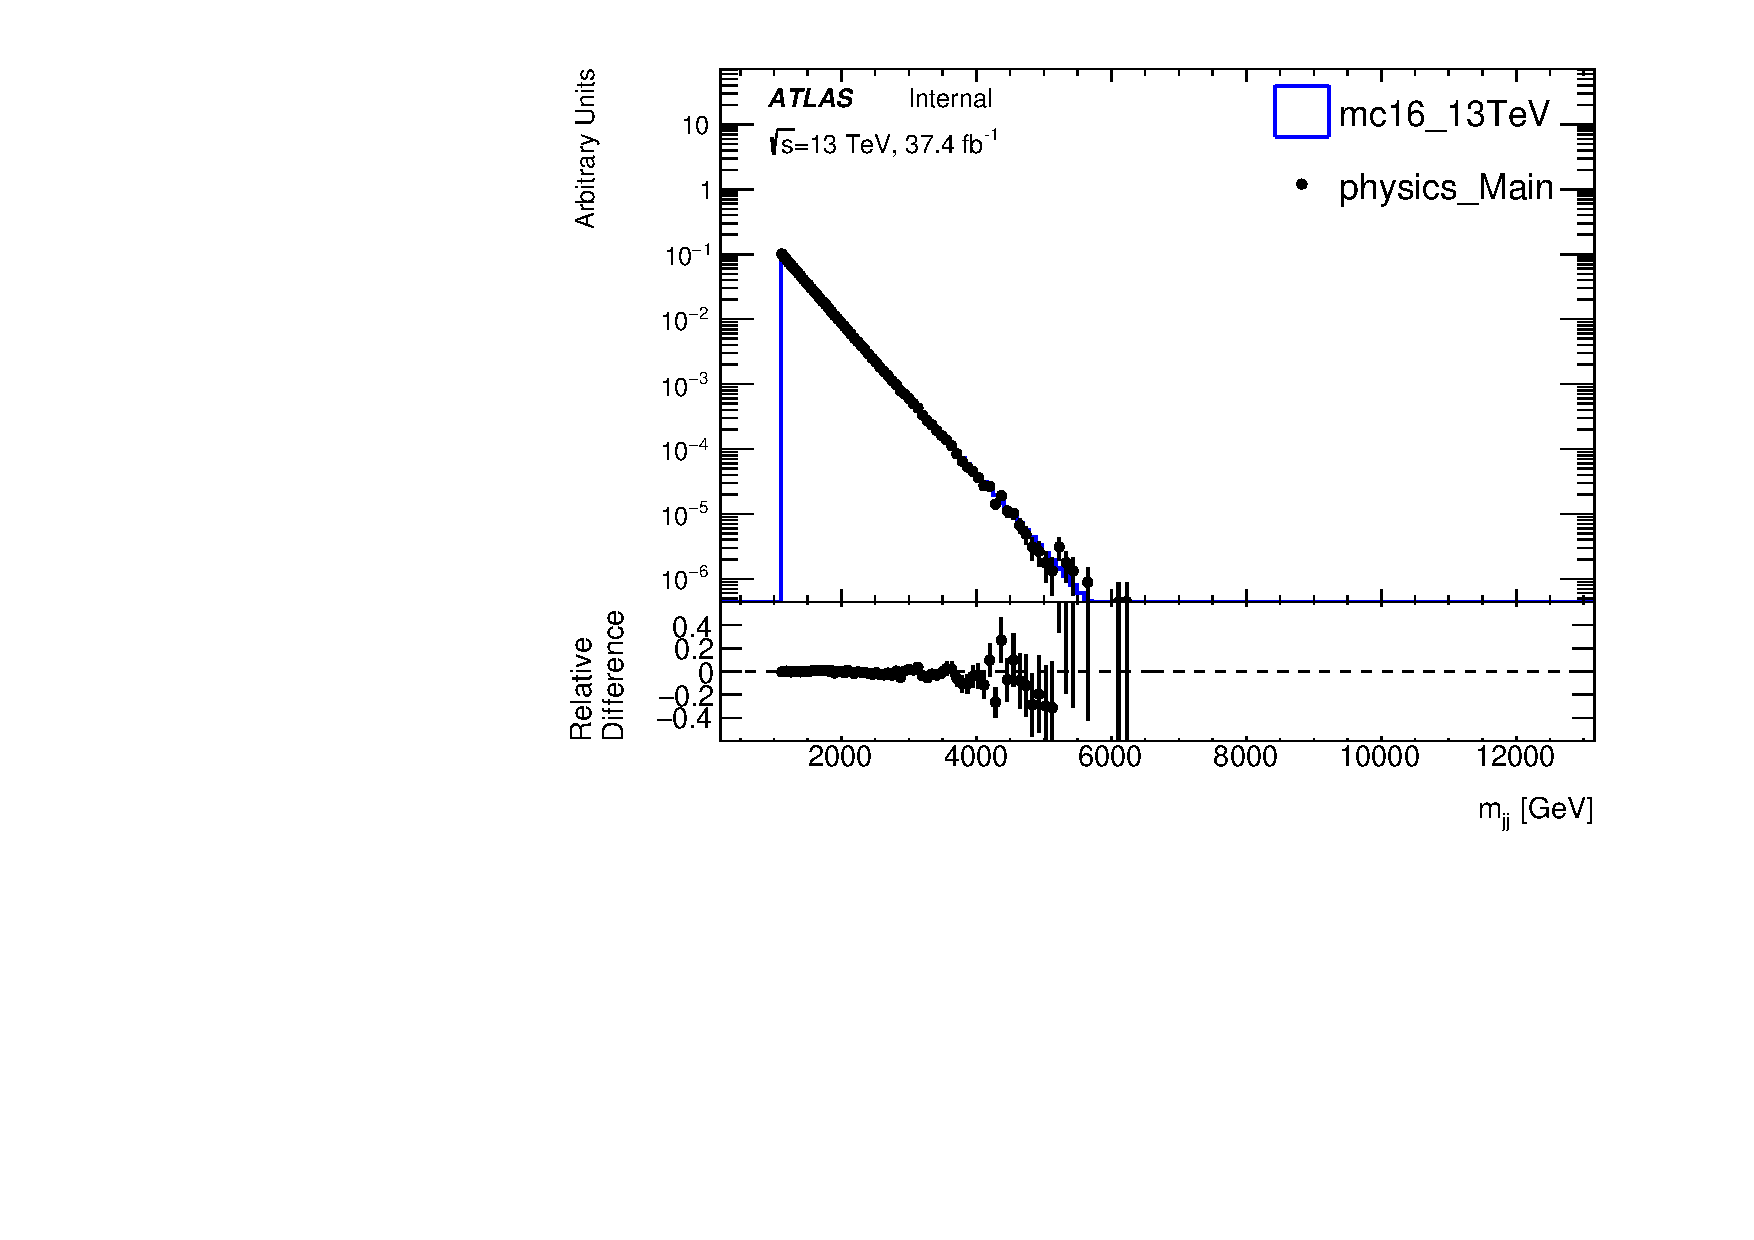
\includegraphics[width=0.45\textwidth]{figures/monitoring/resonant/2015-16/QG/newStudy_mjj_logY_QGv01.pdf}}
 \subfigure[] {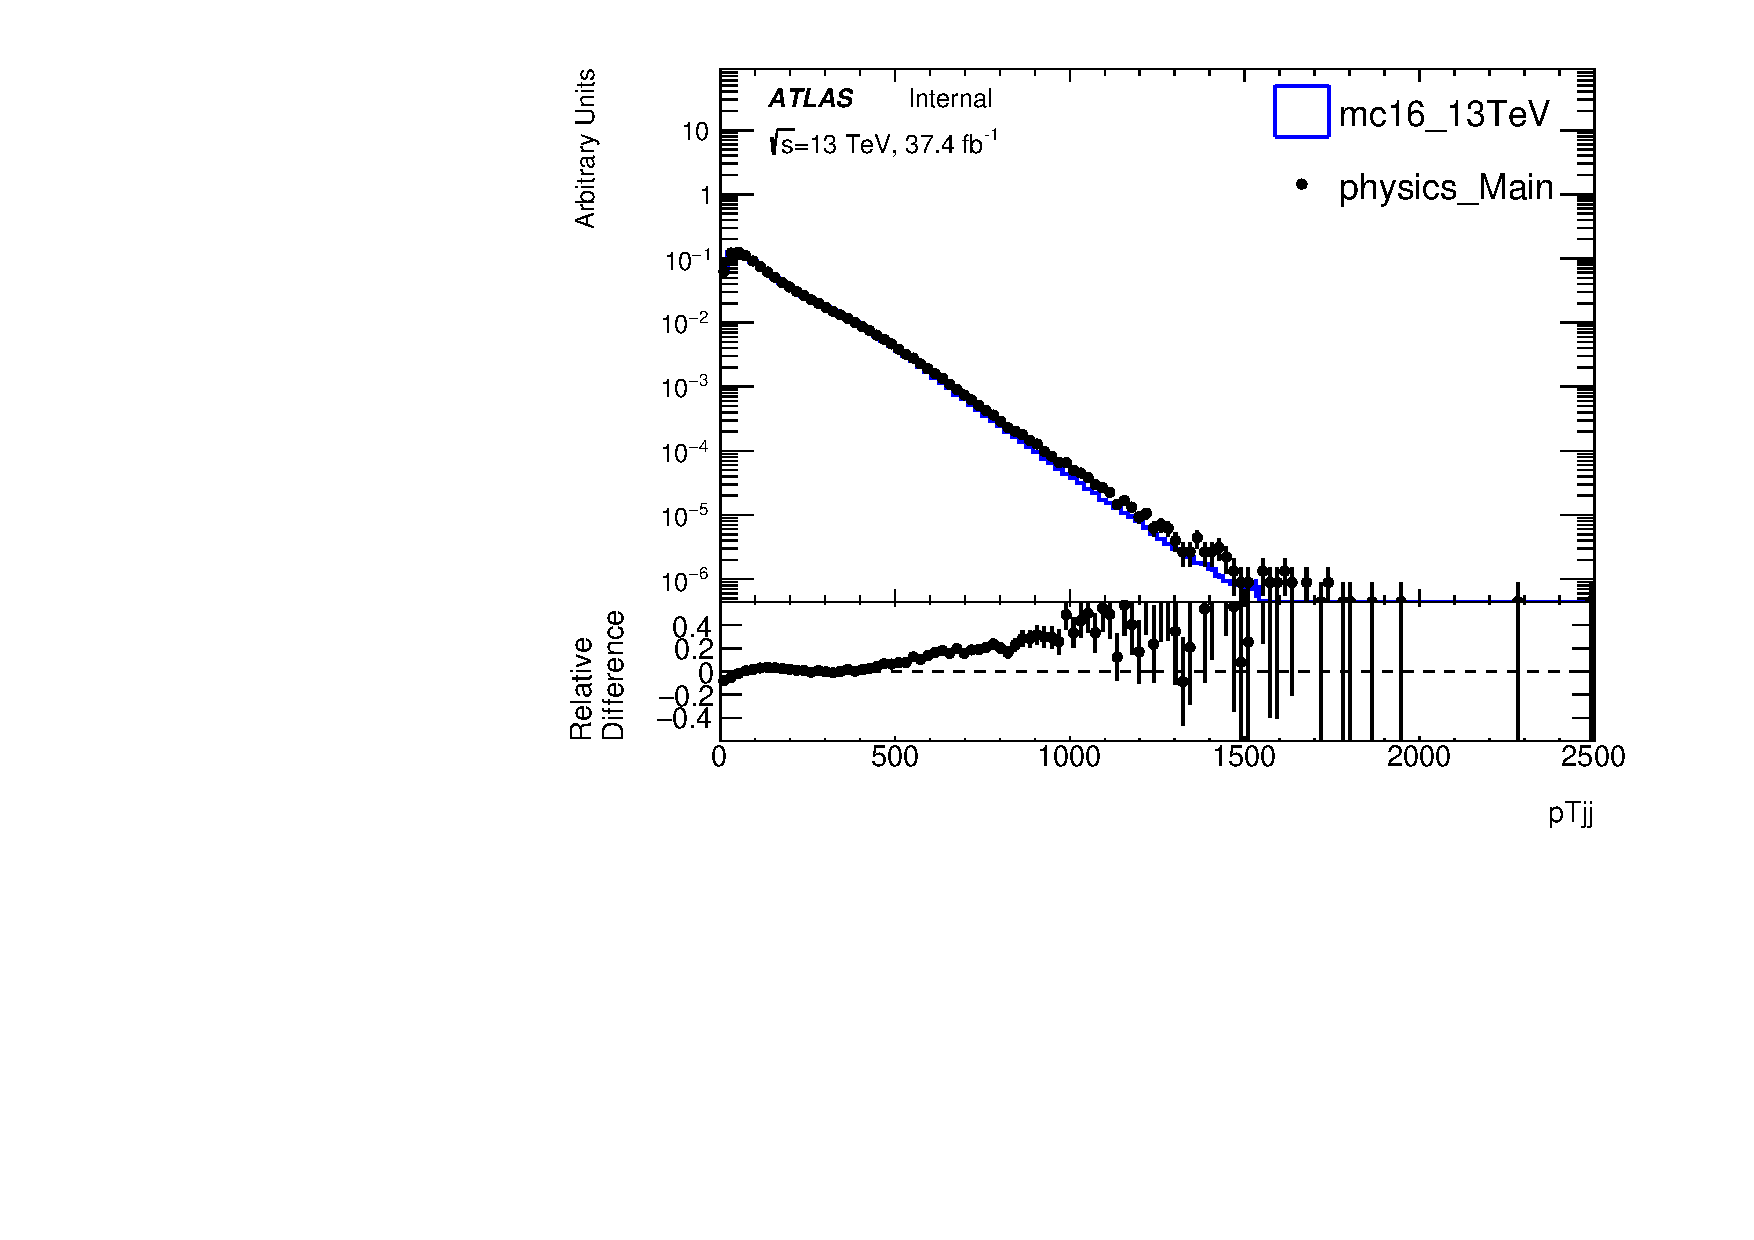
\includegraphics[width=0.45\textwidth]{figures/monitoring/resonant/2015-16/QG/newStudy_pTjj_logY_QGv01.pdf}}
 %
 \subfigure[] {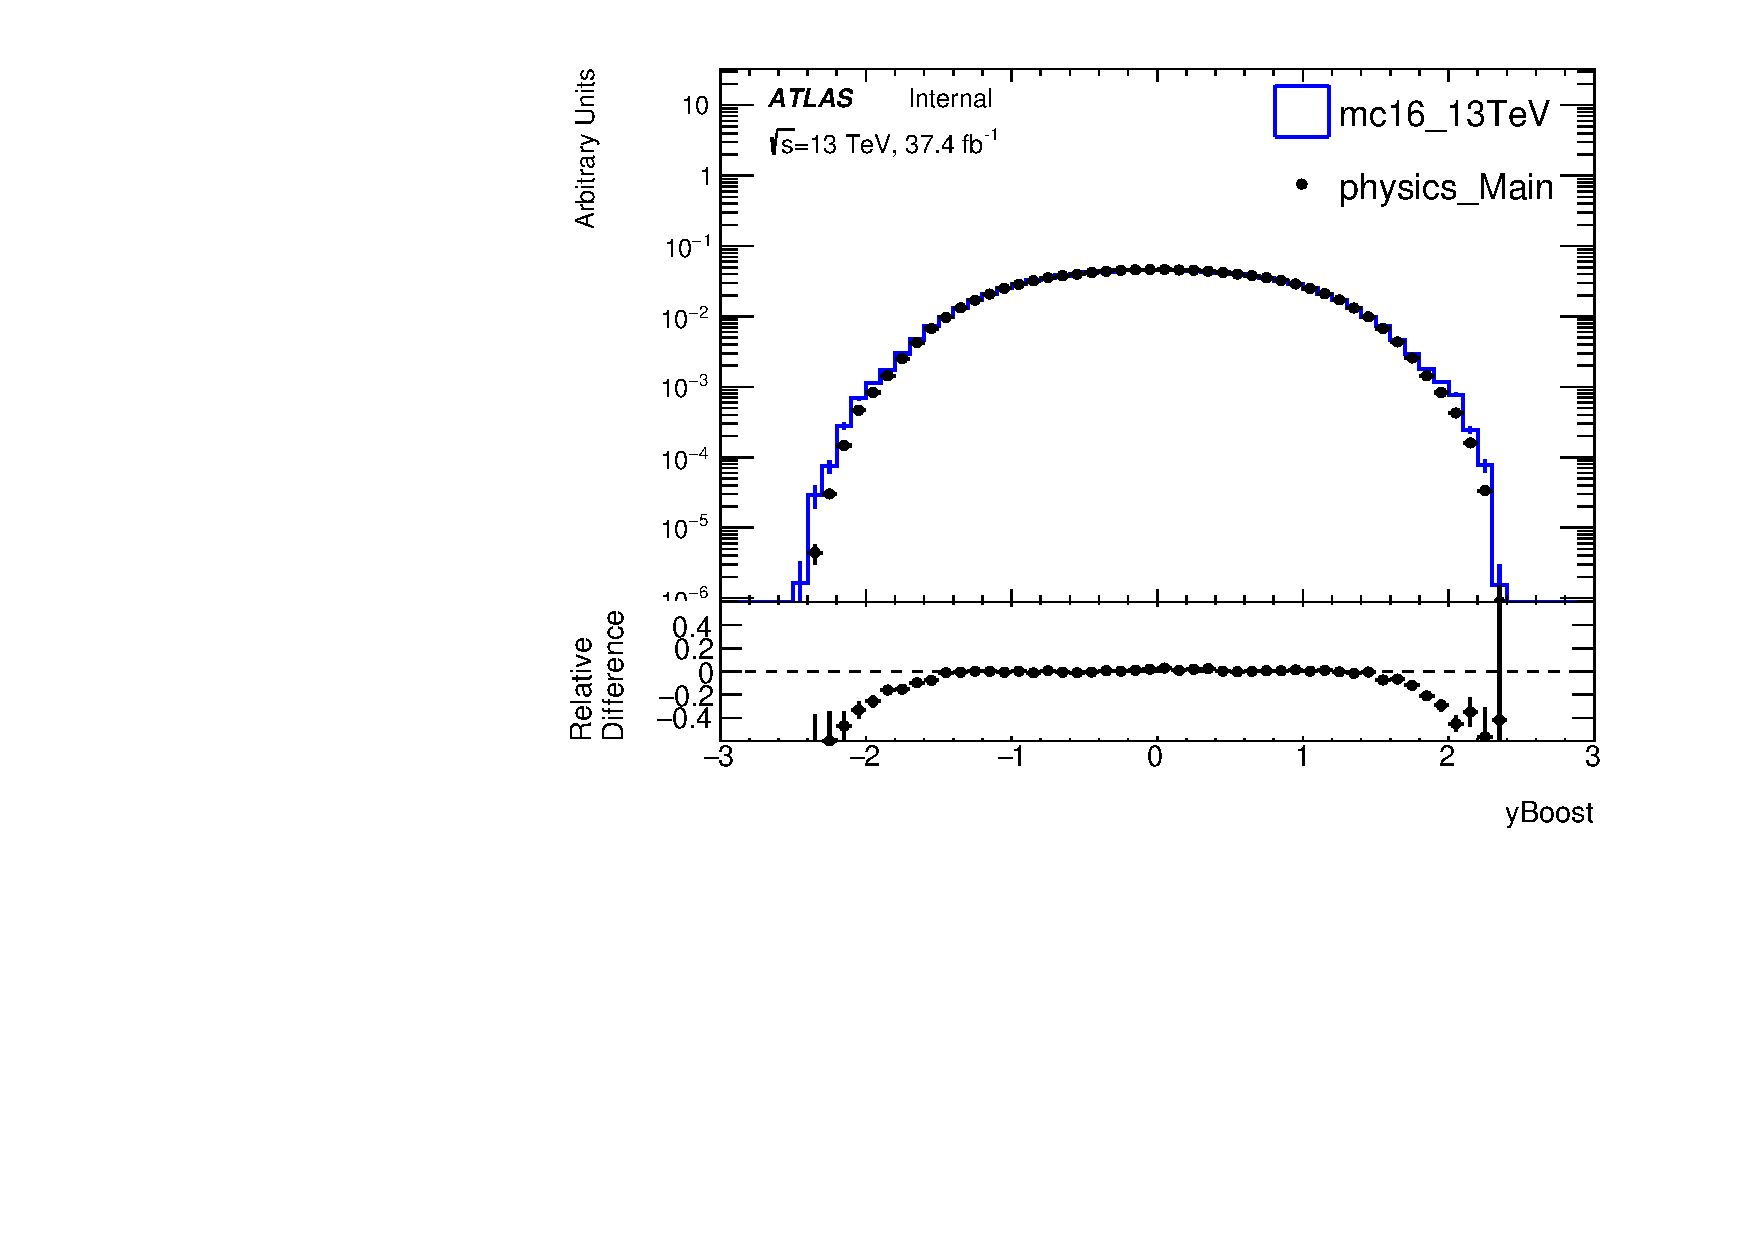
\includegraphics[width=0.45\textwidth]{figures/monitoring/resonant/2015-16/QG/newStudy_yBoost_logY_QGv01.pdf}}
 \subfigure[] {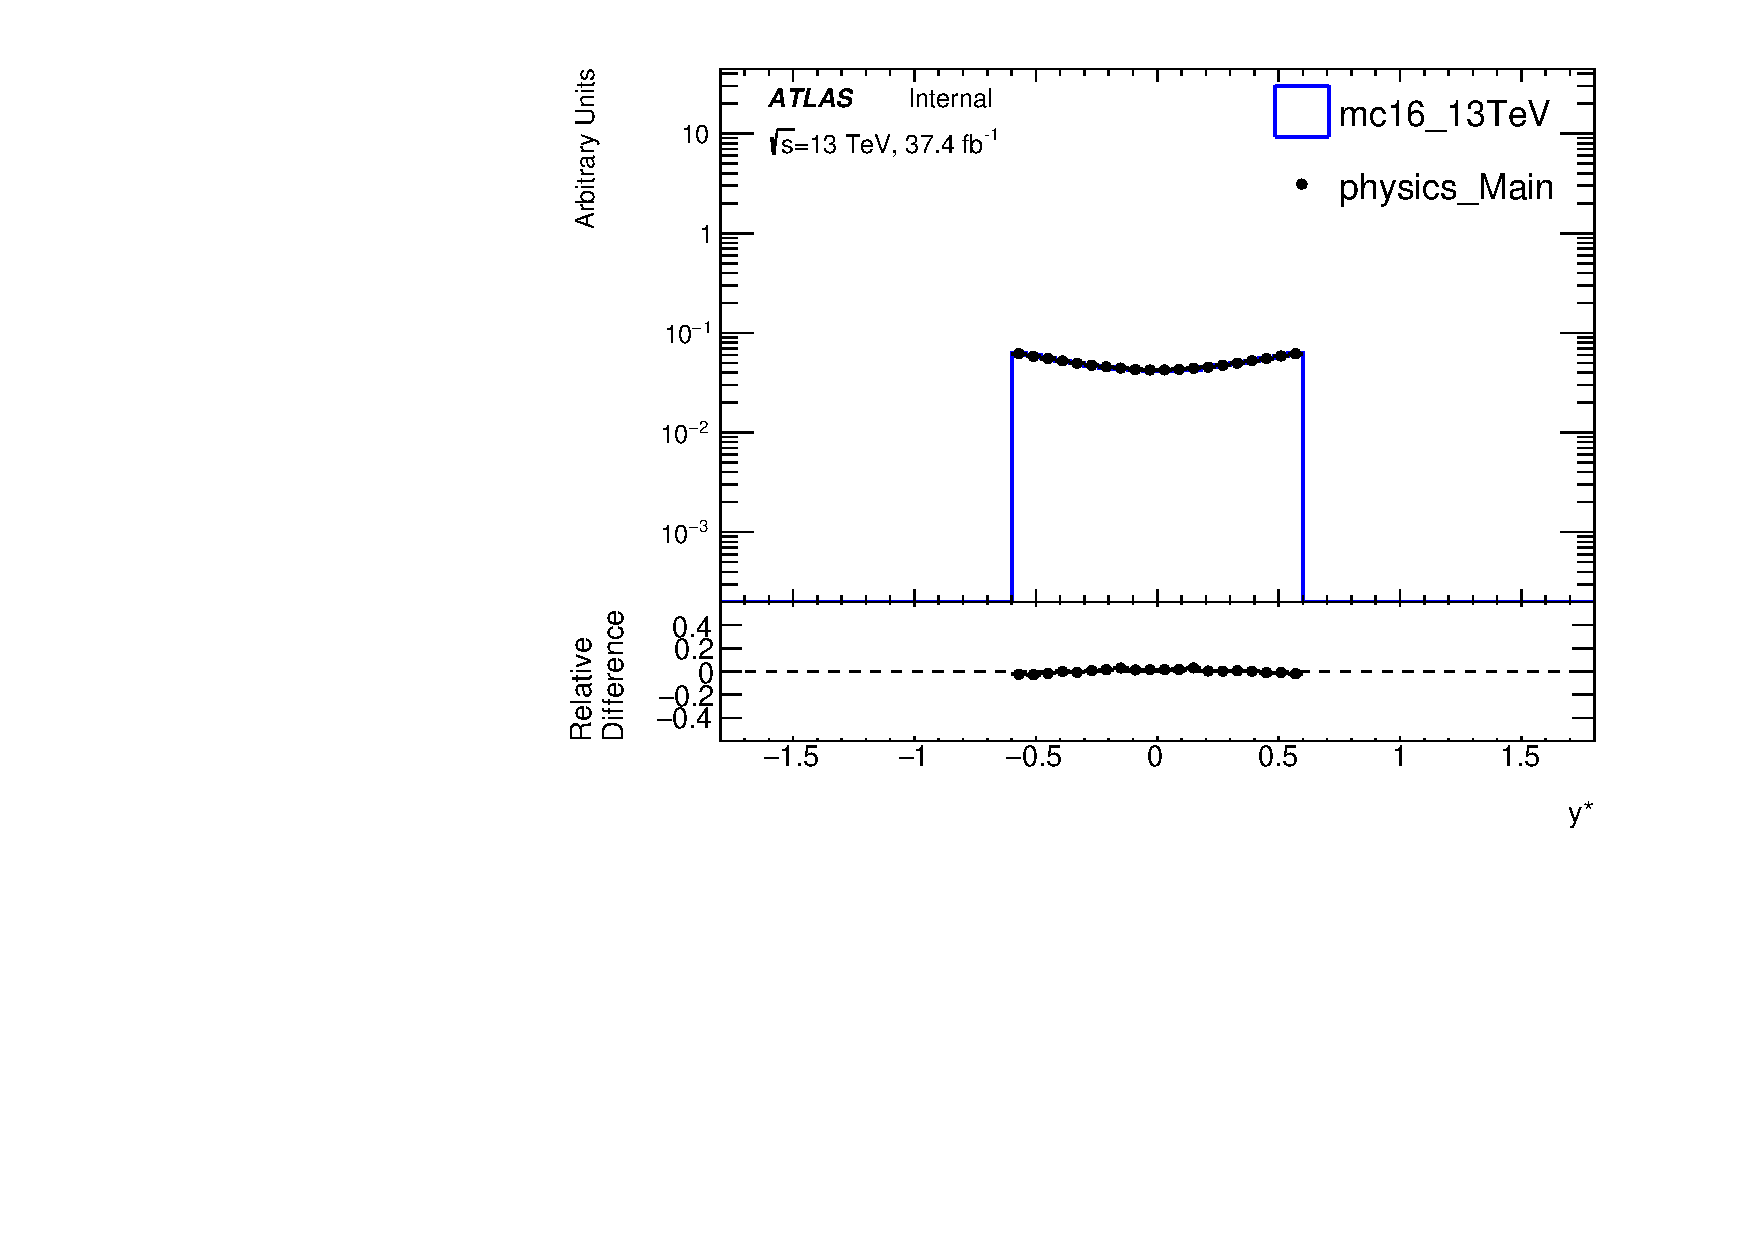
\includegraphics[width=0.45\textwidth]{figures/monitoring/resonant/2015-16/QG/newStudy_yStar_logY_QGv01.pdf}}
 \caption{Jet plots on %2016 data, 
 the resonant selection. (a) dijet invariant mass (b) dijet \pt\ (c) \yB{} (d) \ystar{}. }
 \label{fig:QGmonitoring6}
\end{figure}

\clearpage


In this section a selection of kinematic and monitoring plots produced with the resonant selection on the GG dataset is shown 
(Figures~\ref{fig:GGmonitoring1},  
\ref{fig:GGmonitoring5}, \ref{fig:GGmonitoring6}). These plots are relative to \integLumi of data collected in 2015 and 2016.
 GRL has been applied here.

\begin{figure}[htb]
 \centering
 \subfigure[] {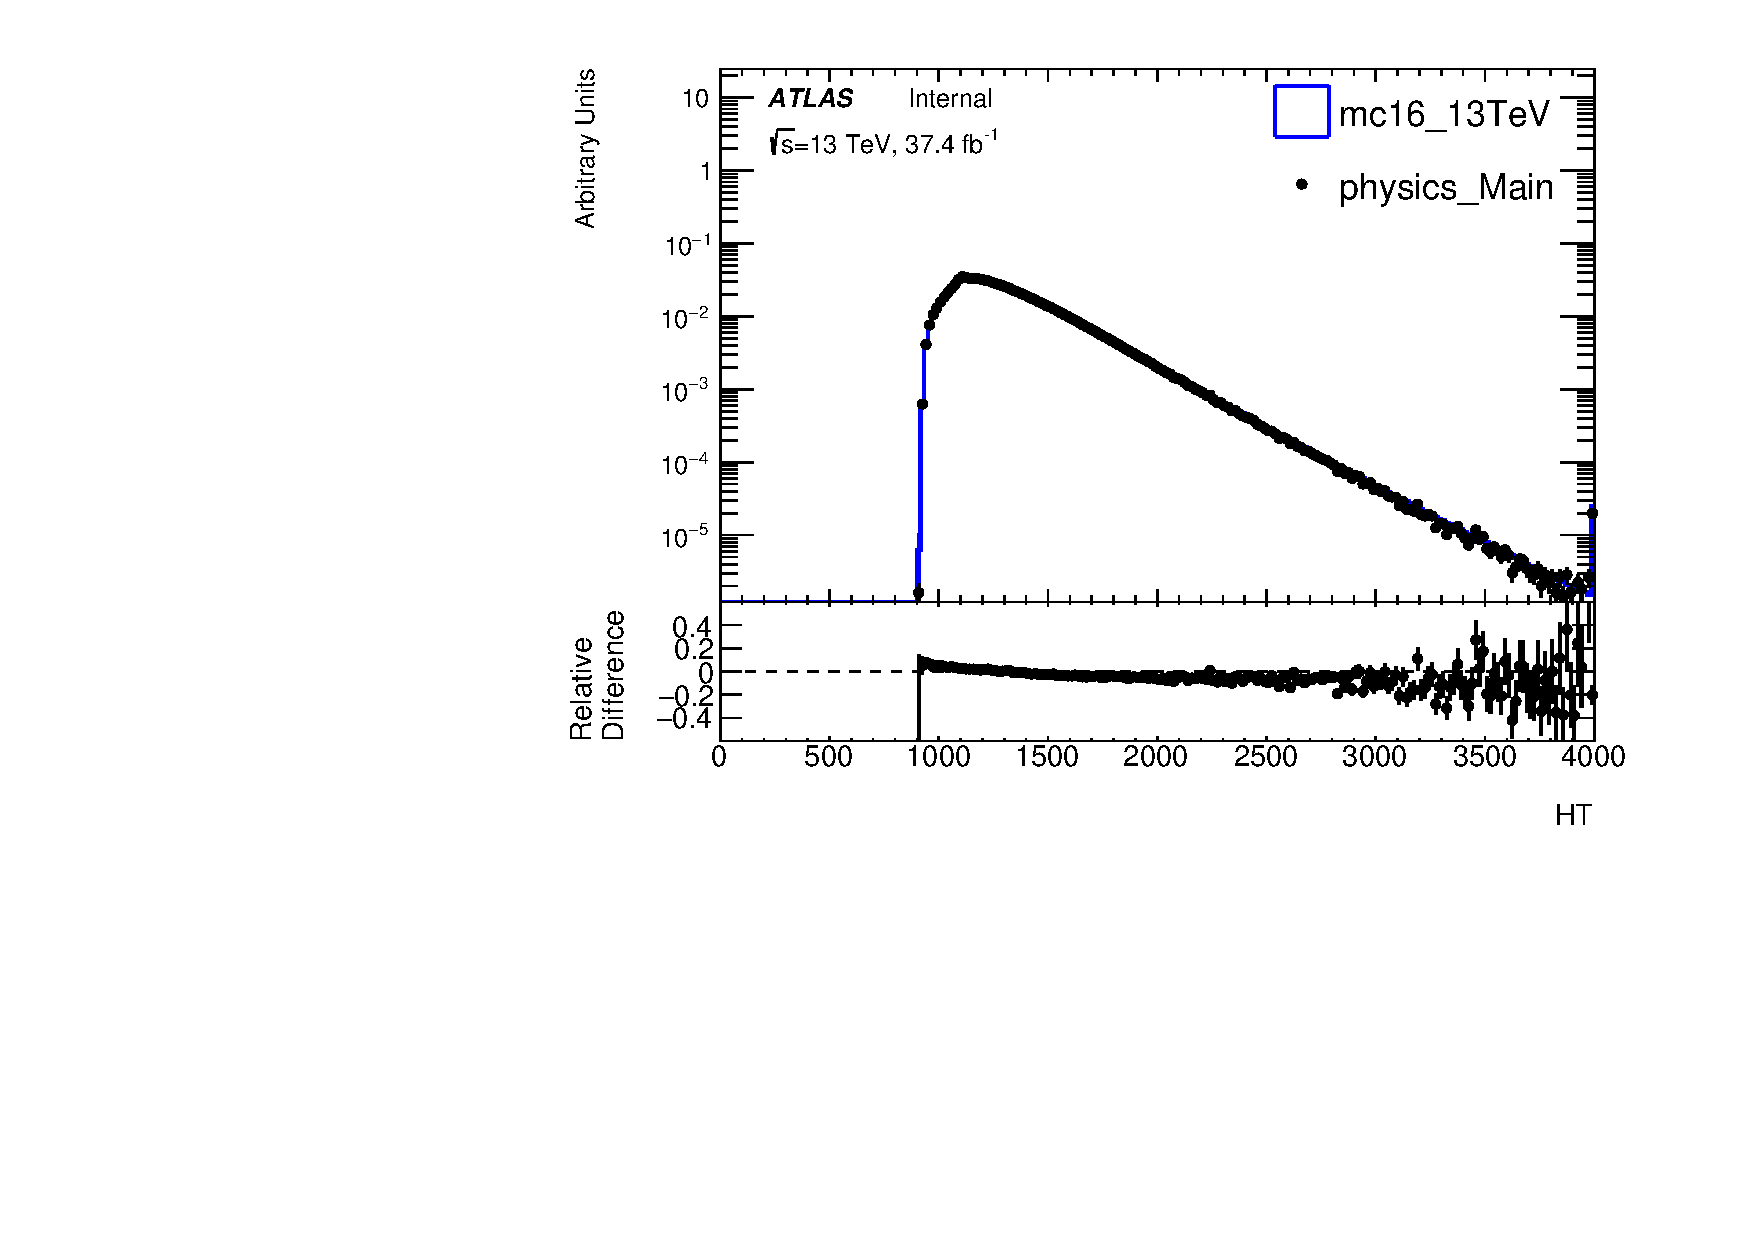
\includegraphics[width=0.45\textwidth]{figures/monitoring/resonant/2015-16/GG/newStudy_HT_logY_GGv01.pdf}}
 \subfigure[] {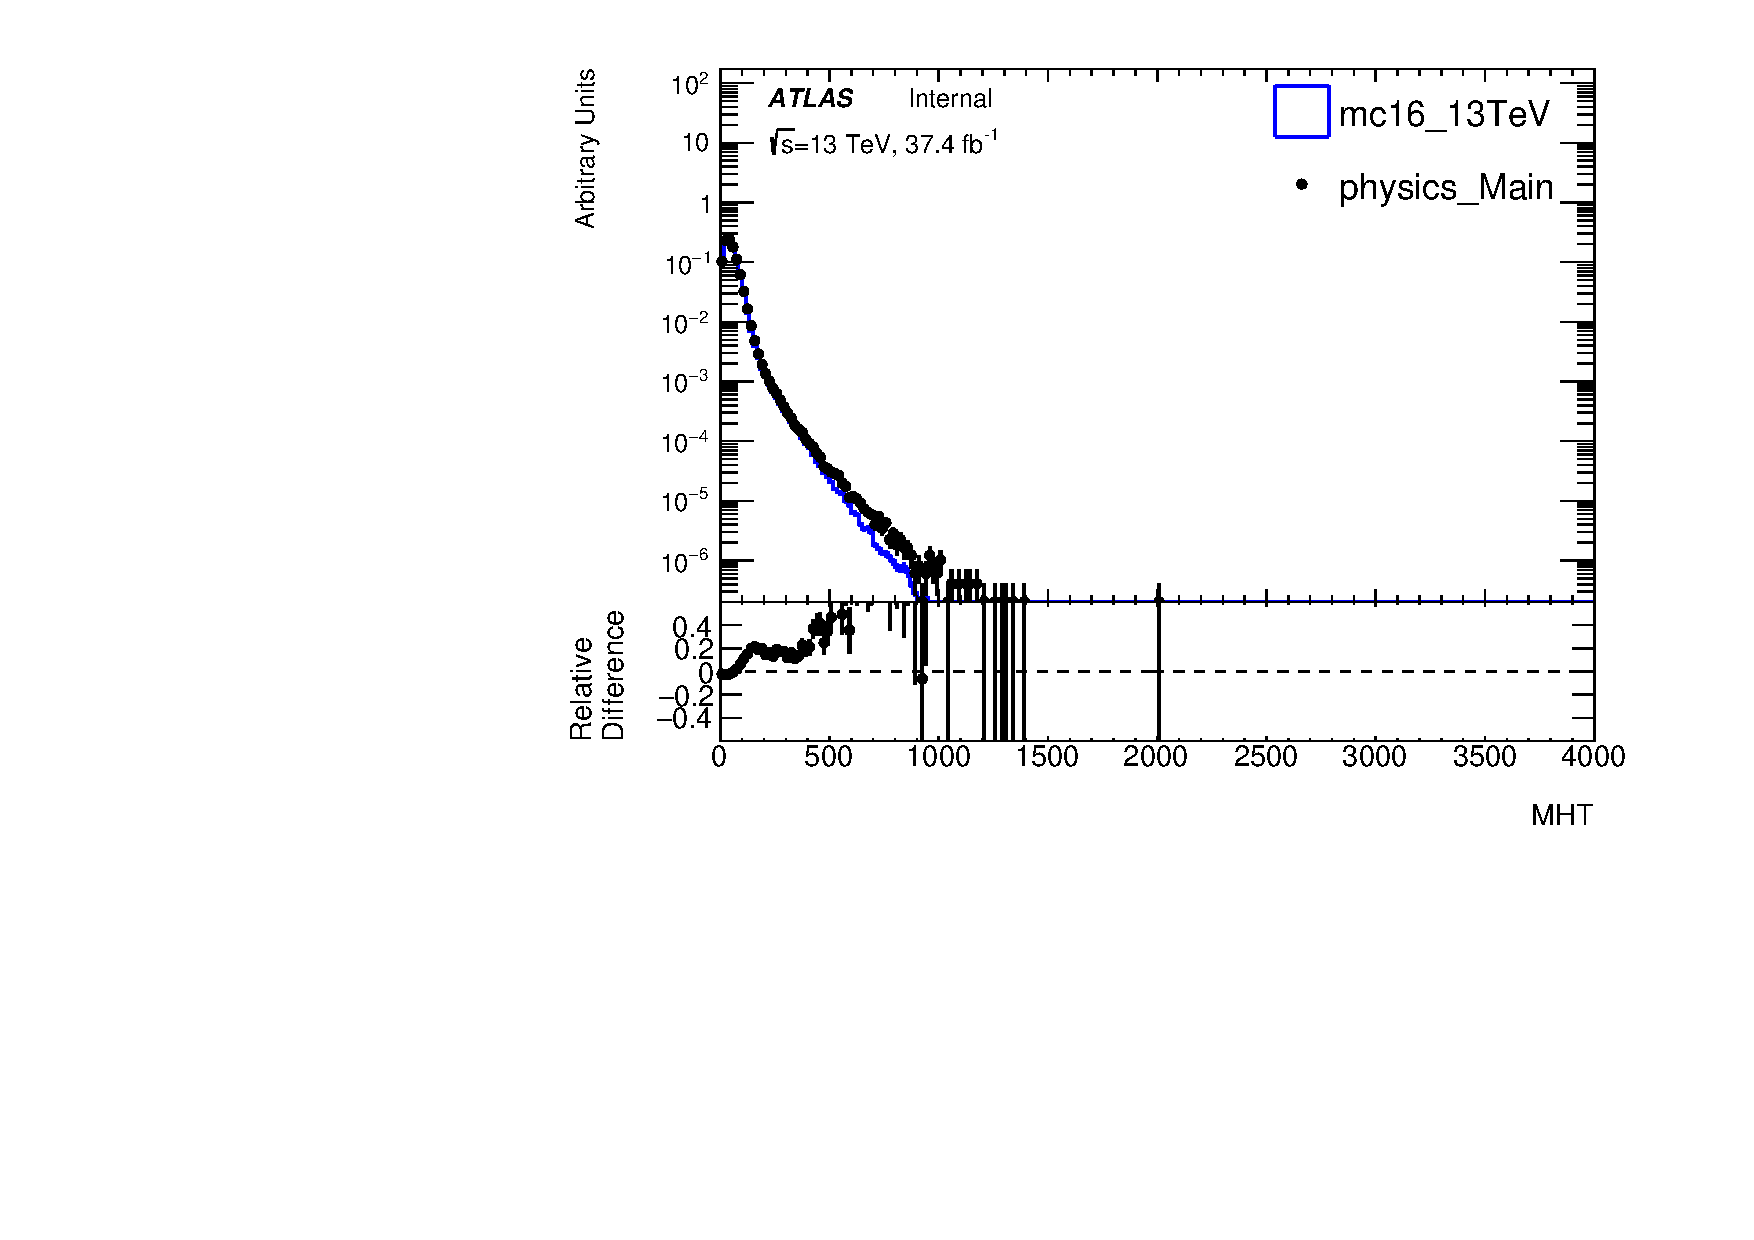
\includegraphics[width=0.45\textwidth]{figures/monitoring/resonant/2015-16/GG/newStudy_MHT_logY_GGv01.pdf}}
 %
 \subfigure[] {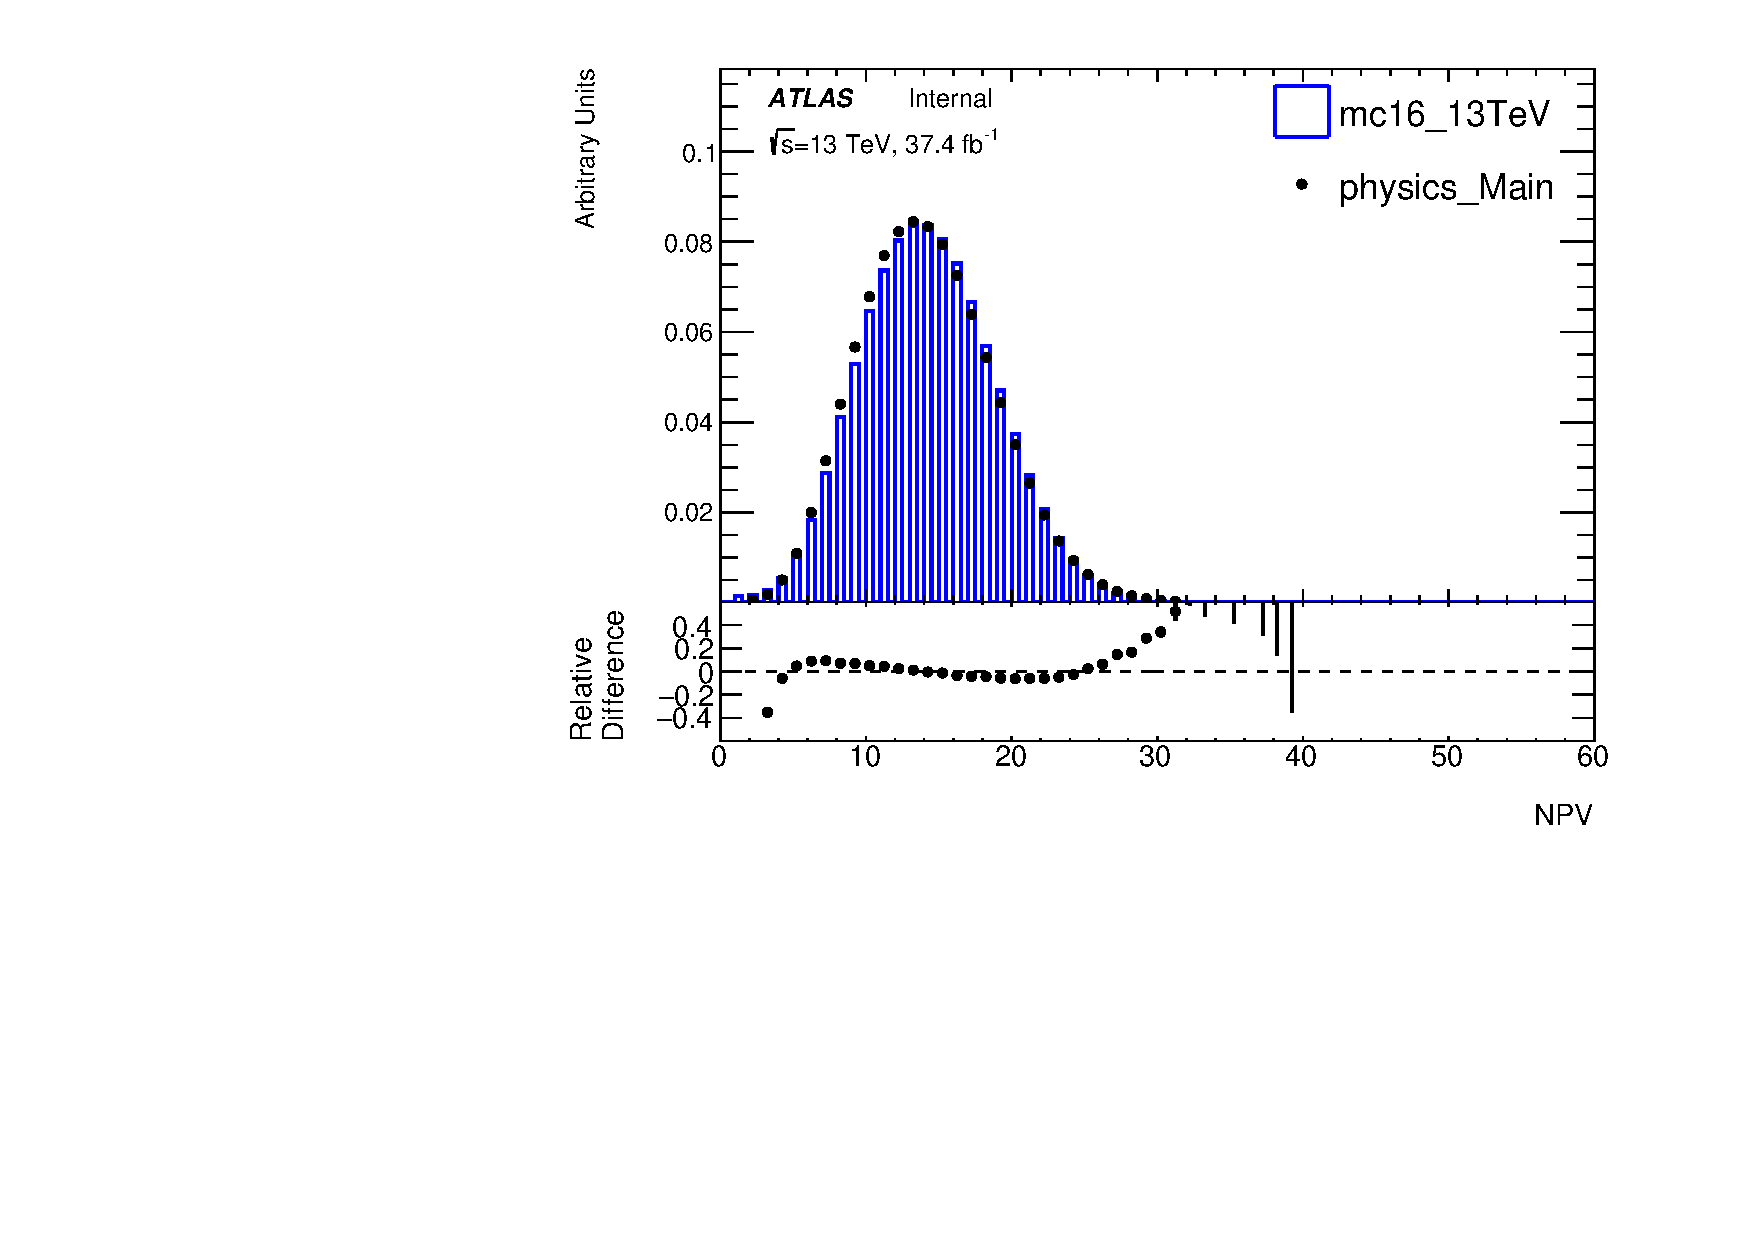
\includegraphics[width=0.45\textwidth]{figures/monitoring/resonant/2015-16/GG/newStudy_NPV_GGv01.pdf}}
 \subfigure[] {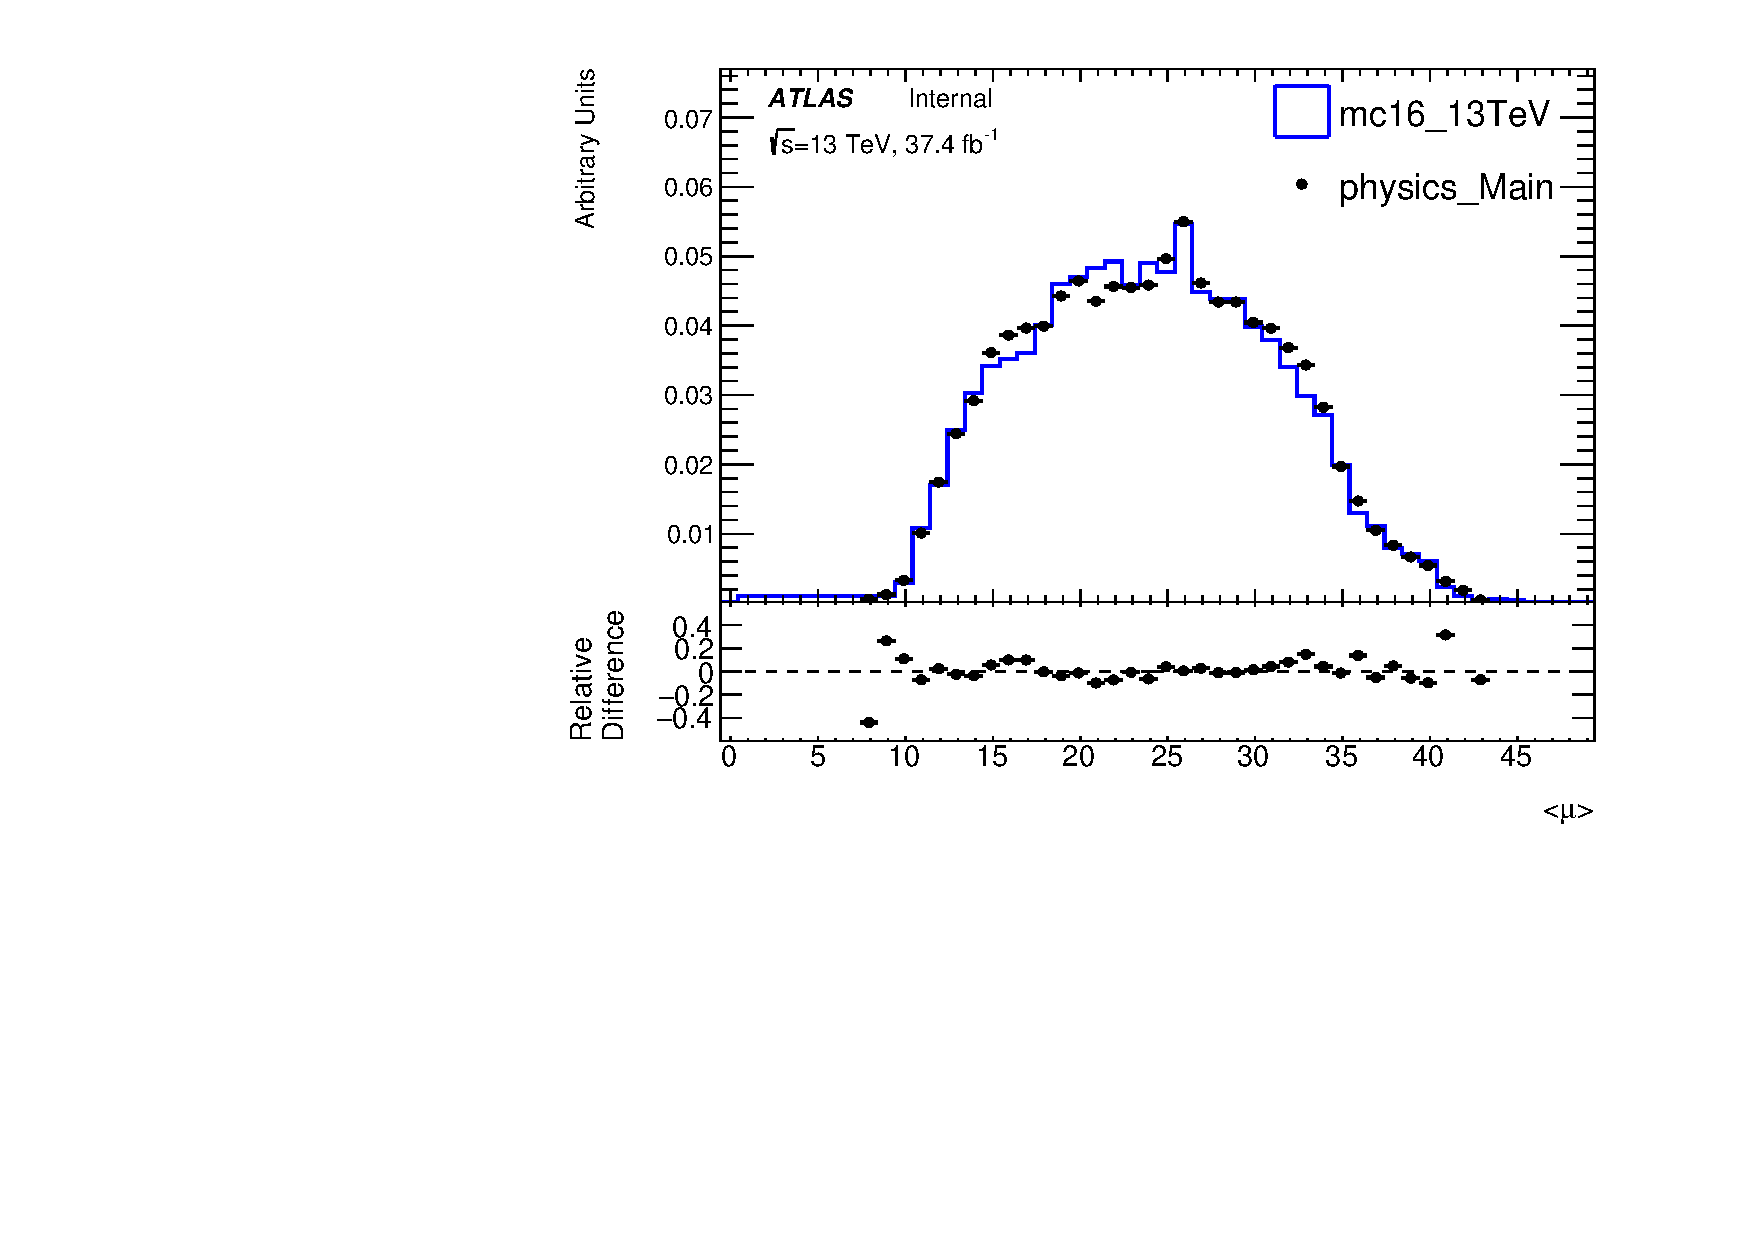
\includegraphics[width=0.45\textwidth]{figures/monitoring/resonant/2015-16/GG/newStudy_averageInteractionsPerCrossing_GGv01.pdf}}
 %

 \caption{Monitoring plots on %2016 data, 
 the GG resonant selection. (a) $H_T$, (b) $MH_T$ (missing transverse momentum calculated only from the jets in the event), (c) number of primary interaction vertices and (d) average interactions per bunch crossing.}
 \label{fig:GGmonitoring1}
\end{figure}

 \begin{figure}[htb]
 \centering
  \subfigure[] {\includegraphics[width=0.45\textwidth]{figures/monitoring/resonant/2015-16/GG/newStudy_njets_GGv01.pdf}}
 \subfigure[] {\includegraphics[width=0.45\textwidth]{figures/monitoring/resonant/2015-16/GG//newStudy_deltaPhi_logY_GGv01.pdf}}
 %
 \subfigure[] {\includegraphics[width=0.45\textwidth]{figures/monitoring/resonant/2015-16/GG/newStudy_jet_eta_logY_GGv01.pdf}}
 \subfigure[] {\includegraphics[width=0.45\textwidth]{figures/monitoring/resonant/2015-16/GG/newStudy_jet_phi_logY_GGv01.pdf}}
 %
 \subfigure[] {\includegraphics[width=0.45\textwidth]{figures/monitoring/resonant/2015-16/GG/newStudy_jet_pt_logY_GGv01.pdf}}
 \subfigure[] {\includegraphics[width=0.45\textwidth]{figures/monitoring/resonant/2015-16/GG/newStudy_jet_rapidity_logY_GGv01.pdf}}
 %
  \caption{Jet plots on %2016 data, 
  the resonant selection. (a) number of jets (b) $\Delta\phi$ between the two jets (c) jet $\eta$
  (d) jet $\phi$ (e) jet \pt\ (f) jet rapidity.  Fluctuations in the jet $phi$ distribution are attributable to dead modules in the tile calorimeter which lead to fewer jets in small slices of the detector.}
 \label{fig:GGmonitoring5}
\end{figure}


 \begin{figure}[htb]
 \centering
 %
 \subfigure[] {\includegraphics[width=0.45\textwidth]{figures/monitoring/resonant/2015-16/GG/newStudy_mjj_logY_GGv01.pdf}}
 \subfigure[] {\includegraphics[width=0.45\textwidth]{figures/monitoring/resonant/2015-16/GG/newStudy_pTjj_logY_GGv01.pdf}}
 %
 \subfigure[] {\includegraphics[width=0.45\textwidth]{figures/monitoring/resonant/2015-16/GG/newStudy_yBoost_logY_GGv01.pdf}}
 \subfigure[] {\includegraphics[width=0.45\textwidth]{figures/monitoring/resonant/2015-16/GG/newStudy_yStar_logY_GGv01.pdf}}
 \caption{Jet plots on %2016 data, 
 the resonant selection. (a) dijet invariant mass (b) dijet \pt\ (c) \yB{} (d) \ystar{}. }
 \label{fig:GGmonitoring6}
\end{figure}

\clearpage

\subsection{Analysis cutflow}
\label{sub:cutflow}

In this section we will present the analysis cutflows. For reference, cutflows obtained on 2015+2016 data using R21 are presented in Table~\ref{tab:cutFlow_resonance_data16}. 
The cut definitions are described in Section~\ref{sec:base_selection} and ~\ref{sec:res_selection}.
The size of the quark-gluon sub-samples are given in Table~\ref{tab:cutFlow_sample_fractions}.

\begin{table}[htbp]
\centering
\sisetup{group-minimum-digits=4}
\begin{tabular}{lSS}
\toprule
Selection criteria & {$N_{events}$} & {rel. decrease (\%)} \\
\midrule
all 	 & 	1682839275	 & 	0.00	 \\
LAr 	 & 	1680323020	 & 	-0.15	 \\
tile 	 & 	1680232308	 & 	-0.01	 \\
core 	 & 	1679301246	 & 	-0.06	 \\
NPV 	 & 	1678594582	 & 	-0.04	 \\
Trigger (OR) 	 & 	1520215165	 & 	-9.44	 \\
2 jets $\pt>60~\GeV$    	 & 	1409142270	 & 	-7.31	 \\
$\mathrm{jet}_{1} \pt>360~\GeV$  	 & 	150694315	 & 	-89.31	 \\
Apply GRL	 & 	147028750	 & 	-2.43	 \\
HLT j380 	 & 	110618942	 & 	-24.76	 \\
cleaning 	 & 	110618942	 & 	0.00	 \\
$\mathrm{jet}^{\mathrm{lead}}_{\pt}>440~\GeV$	 & 	54863611	 & 	-50.40	 \\
$\mjj >1100~\GeV$	 & 	27303100	 & 	-50.23	 \\
$|y* < 0.6|$	 	 & 	7533433	 & 	-72.41	 \\
\bottomrule
\end{tabular}
\caption{Cutflow for  
events with resonance cuts: $\mathrm{jet}^{\mathrm{lead}}_{\pt}>440~\GeV$, $m_{jj}>1100~\GeV$, and $|y*|<0.6$. 
"Trigger" corresponds to the events passing the OR of L1\_J75, L1\_J100, HLT\_j360, HLT\_j380, HLT\_j400 (and HLT\_3j175, HLT\_4j85, and HLT\_4j100 for 
neighbouring analyses using 3 or 4 jet topologies).
\label{tab:cutFlow_resonance_data16} }
\end{table}




\begin{table}[htbp]
\sisetup{group-minimum-digits=4}
\centering
\begin{tabular}{lSS}
Data Set 	& \multicolumn{1}{c}{$N_{\mathrm{events}}$} 	& \multicolumn{1}{c}{Fraction (\%)} \\
\hline
QQ 			& 313113 		& 4.2\\
QG			& 2275205 		& 30.2\\
GG			& 4945115	  	& 65.6\\
\hline\hline
\end{tabular}
\caption{Fraction of 2015+12016  events with resonance cuts in the quark-quark (QQ), quark-gluon (QG) and gluon-gluon (GG)
sub-samples. 
\label{tab:cutFlow_sample_fractions} }
\end{table}




